\chapter{概要}
\section{程序}
\begin{figure}[H]
\centering
\begin{subfigure}{.48\textwidth}
\centering
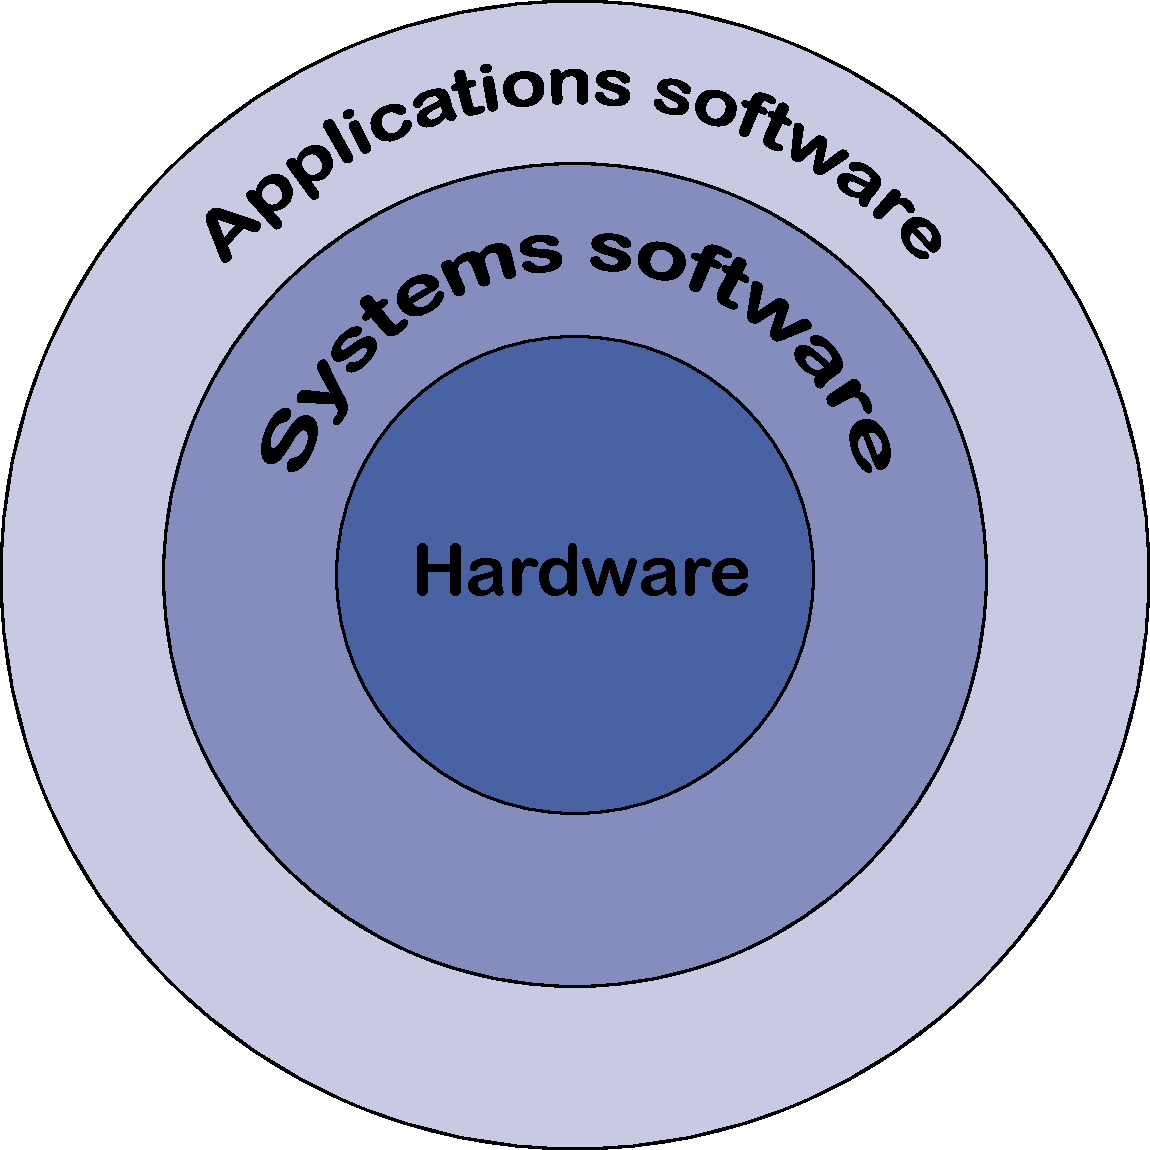
\includegraphics[scale=.2]{img/figure17.pdf}
\caption{简化的硬软件层次结构}
\end{subfigure}
\begin{subfigure}{.48\textwidth}
\centering
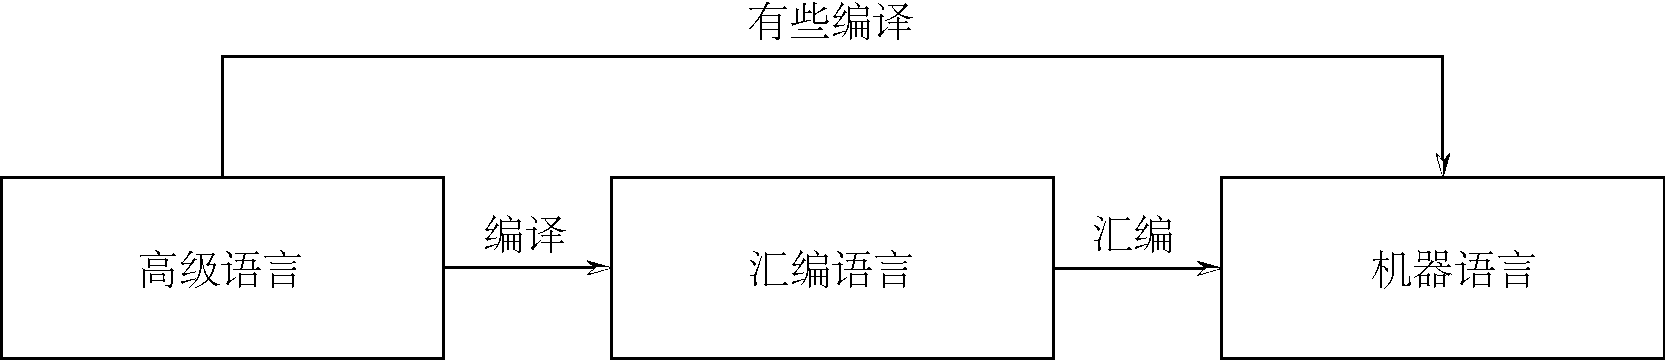
\includegraphics[scale=.3]{img/figure18.pdf}
\caption{从高级语言到机器语言}
\end{subfigure}
\end{figure}
\begin{itemize}
\item 应用软件 \par 用高级语言编写
\item 系统软件
\begin{itemize}
\item 操作系统 \par 处理\verb|I/O|, 分配内存, 为应用程序提供服务
\item 编译程序
\end{itemize}
\item 硬件 \par 处理器, 主存, 输入输出系统等
\end{itemize}
\section{硬件}
计算机的核心硬件是\verb|CPU|(控制器和\verb|ALU|), 存储器(主存和外存), \verb|I/O|设备. 其中, 较受到关注的\verb|I/O|设备有:
\begin{itemize}
\item 鼠标
\begin{itemize}
\item 电动机械式: 一个球滚动
\item 光电式: \verb|LED|光源, 每秒\verb|1500|次采样, 处理器进行照片对比
\end{itemize}
\item 显示器 \par 图像的像素矩阵用位图表示, 分辨率是\verb|x|, \verb|y|轴上点的个数. 彩色显示器每种颜色可以用\verb|8|位二进制数表示, 每像素\verb|RGB|三色, 故每像素用\verb|24|位表示. 图像保存在帧缓存中, 一幅图像为一帧
\begin{itemize}
\item 液晶显示器 \par 每个像素由一个三极管控制光线是否通过, 三个三极管控制颜色分配, 共四个三极管. 不施加电压是透光, 施加电压是不透光
\end{itemize}
\end{itemize}
\section{性能}
\begin{itemize}
\item 机器字长 \par 计算机进行一次整数运算能处理的二进制位数, 通常和\verb|CPU|的寄存器位数/加法器有关.
\item 数据通路带宽 \par 数据总线(非\verb|CPU|内部总线)一次能传递信息的位数.
\item 主存容量
\begin{itemize}
\item \verb|MAR|: 主存地址, 反映存储单元的个数
\item \verb|MDR|: 主存数据, 反映存储单元的位数
\end{itemize}
\item 运算速度
\begin{itemize}
\item 响应时间: 计算机完成某任务需要的总的时间
\begin{itemize}
\item \verb|CPU|执行时间
\begin{itemize}
\item 用户\verb|CPU|时间: 程序本身花费的时间, 体现\verb|CPU|性能(重点研究)
\item 系统\verb|CPU|时间: 操作系统的时间, 体现系统性能
\end{itemize}
\item 等待\verb|I/O|等或多任务时其他程序运行的时间
\end{itemize}
\item 吞吐量 \par 单位时间那完成的任务量
\item 时钟周期 \par 常数. 又称节拍. 时钟频率=1/时钟周期
\item \verb|Average CPI(clock cycles per instruction)| \par 一个程序或者程序片段的全部指令所有时钟周期数的平均值.
\end{itemize}
\end{itemize} \par
看了上面一些性能衡量的指标, 所以\textbf{到底}我们应该怎么衡量性能呢?--下面的公式: \par 
\begin{center}
\verb|Average CPI = CPU时钟周期数 / 指令数|\\
\verb|一个程序的CPU执行时间 = 指令数 * Average CPI * 时钟周期|\\
\verb|性能 = 1 / 一个程序的CPU执行时间|
\end{center}
\section{功耗}
\verb|CMOS|集成电路的动态功耗计算:
\begin{center}
\verb|动态功耗 = 负载电容 * 电压^2 * 开关频率|
\end{center}\par
从上面的公式看出, 我们可以通过下降电压来降低功耗, 但是降低电压会导致``漏电''现象. 同时, 电压过高会导致散热问题难以解决. 所以, 我们采用了一种方法: 多核处理器.
\section{性能测试方法}
\begin{itemize}
\item \verb|SPEC CPU|基准测试程序 \par
\verb|SPEC(System Performance Evaluation Coorperative)| 为\verb|CPU, I/O, Web,...|等开发了若干用于测试性能的程序, 我们只要选择一种处理器作为基准处理器, 按照下面的公式即可测试性能:
\begin{center}
\verb|SPECratio = 参考处理器执行时间 / 被测计算机执行时间|\\
\verb|性能测试结果 = SPECratio的几何平均值|
\end{center}
\item 功耗基准测试程序 \par
性能用吞吐率\verb|ssj_ops|表示, 即每秒钟的操作次数. 现在, 我们将负载设为\verb|0|, 同时记录\verb|ssj_ops|, 将负载提高\verb|10%|, 记录\verb|ssj_ops|, 再将负载提高\verb|10%|, 再记录\verb|ssj_ops|,...如此循环往复, 直到满负载. 得到的结果用以下公式计算:
\begin{center}
\verb||
\end{center}
\begin{equation*}
\symtt{\text{\texttt{功耗测试结果}} = \frac{\sum_{i=0}^{10}ssj\_ops_{i}}{\sum_{i=1}^{10}power_{i}}}
\end{equation*}
\end{itemize}
\section{\texttt{Amdahl}定律}
首先, 要解释以下几个变量的含义:
\begin{itemize}
\item \verb|T_0|: 改进前的总执行时间
\item \verb|T_improved|: 改进后的总执行时间
\item \verb|T_affected|: 受改进影响的执行时间
\item \verb|T_unaffected|: 未受改进影响的执行时间
\end{itemize}\par
根据上面的几个变量, 衍生出了下面的几个变量:
\begin{itemize}
\item 可改进比\verb|Fe| \par \verb|Fe = T_affected / T_0|
\item 加速比\verb|Sn| \par \verb|T_0 / T_improved|
\item 部件加速比\verb|Se|(改进量) \par \verb|T_affected / (T_improved - T_unaffected)|
\end{itemize}\par
下面就是著名的\verb|Amdahl|定律:
\begin{center}
\verb|T_improved = T_affected / Se + T_unaffected|
\end{center}\par
当然, 这个公式还有其他改进:\vspace{1em}
\begin{equation*}
\symtt{\frac{1}{\sum_{i=1}^{m}\frac{Fe_{i}}{Se_{i}}+(1-\sum_{i=1}^{m}Fe_{i})}}, \text{\texttt{其中i表示改进的部件的数量}}
\end{equation*}
\chapter{指令}
\section{引言}
\paragraph{指令集}~{一个给定的计算机体系结构所包含的指令集合} 
\paragraph{汇编语言和机器语言}~{前者是编程的书写形式, 后者是计算机所能识别的形式} 
\paragraph{存储程序}~{多种类型的指令和数据均以数字形式存储在存储器(内存)中}
\paragraph{\texttt{MIPS}}~{是一种汇编语言, 属于精简指令集}
\section{硬件操作}
\subsection{\texttt{MIPS}汇编指令}
\begin{itemize}
\item 每条\texttt{MIPS}算数运算指令只执行一个操作
\item 一行写一条命令
\item \#后是注释
\end{itemize}
\subsection{高级语言与编译语言之间的关系}
高级语言经过编译器编译, 形成汇编语言.
\section{\texttt{MIPS}寄存器及常用指令}
高级语言的变量数量不受限制, 而汇编语言逻辑运算指令的变量对应寄存器, 而寄存器数量有限, 故变量数量受限.
\subsection{寄存器}
\begin{itemize}
\item 共有\verb|32|个寄存器, 编号为\verb|0-31|
\item \verb|32bit|数据称为一个``字'', \verb|32|位为字长, 每个字\verb|4|字节
\item 按字节编址
\item 寄存器分类型:
\begin{itemize}
\item \verb|$ZERO|: 恒为\verb|0|
\item \verb|$v0-$v1|: 返回值
\item \verb|$a0-$a3|: 参数
\item \verb|$t0-$t9|: 临时变量, 其中\verb|$t0-$t7|对应编号\verb|8-15|, \verb|$t8-$t9|对应编号\verb|24-25|, 无需压栈
\item \verb|$s0-$s7|: 保留变量, 对应编号\verb|16-23|, 必须压栈
\item \verb|$gp|: 静态数据的全局指针
\item \verb|$sp|: 栈指针
\item \verb|$fp|: 帧指针
\item \verb|$ra|: 返回地址
\end{itemize}
\end{itemize}
\subsection{常见指令}
复杂的数据结构(数组等)存储于存储器中, 需要用数据传输指令交换数据:
\begin{itemize}
\item \verb|lw rt, shamt(rs)|: 取数
\item \verb|sw rs, shamt(rt)|: 存数
\end{itemize}\par
数据被存储到寄存器后, 可以进行相加减:
\begin{itemize}
\item \verb|add rd, rs, rt|: 加法
\item \verb|sub rd, rs, rt|: 减法
\end{itemize}\par
我们经常要在加减运算的时候用到常数, 这样就会导致计算机会去内存中取出这个常数存储到寄存器这一多余的步骤, 可以通过立即数以除去这一过程:
\begin{itemize}
\item \verb|addi rt, rs, constant|: 加立即数
\item \verb|-addi rt, rs, constant|: 没有减立即数, 用这个替代
\end{itemize}\par 
特殊的, 如果我们要进行寄存器间的赋值, 可以通过\verb|add|或者\verb|addi|实现:
\begin{itemize}
\item \verb|add rd, rs, $ZERO|: 将\verb|rs|赋值给\verb|rd|
\item \verb|addi rt, rs, 0|: 将\verb|rs|赋值给\verb|rt|
\end{itemize}
\section{\texttt{MIPS}指令格式}
指令包含操作码和地址码.
\subsection{\texttt{R}型指令}
\begin{table}[H]
\centering
\begin{tabularx}{\textwidth}{|Z|Z|Z|Z|Z|Z|}
\hline
op & rs & rt & rd & shamt & funct  \\
\hline
\end{tabularx}
\end{table} \par 
他们的作用:
\begin{itemize}
\item \verb|op|: 操作码
\item \verb|rs|: 第一个源寄存器号
\item \verb|rt|: 第二个源寄存器号
\item \verb|rd|: 目标寄存器号
\item \verb|shamt|: 位移量
\item \verb|funct|: 功能码(与\verb|op|一起起作用)
\end{itemize} \par 
他们的位数:
\begin{itemize}
\item \verb|op|: \verb|6|位, 因为有\verb|64|种指令
\item \verb|rs,rt,rd|: \verb|5|位, 因为有\verb|32|个寄存器
\item \verb|shamt|: \verb|5|位, 因为\texttt{MIPS}是\verb|32|位指令
\item \verb|funct|: \verb|6|位, 因为\verb|32-6-5-5-5-5=6|
\end{itemize}\par
上述操作码可以查询表格, 寄存器号需要记忆, 下面也一样.
\subsection{\texttt{I}型指令}
\begin{table}[H]
\centering
\begin{tabularx}{\textwidth}{|Z|Z|Z|p{15em}<{\centering}|}
\hline
op & rs & rt & constant or address \\
\hline
\end{tabularx}
\end{table}\par
他们的作用:
\begin{itemize}
\item \verb|op|: 操作码
\item \verb|rs|: 源寄存器号
\item \verb|rt|: 目标寄存器号
\item \verb|constant or address|: 偏移量
\end{itemize}\par
他们的位数:
\begin{itemize}
\item \verb|op|: \verb|6|位, 因为有\verb|64|种指令
\item \verb|rs,rt|: \verb|5|位, 因为有\verb|32|个寄存器
\item \verb|constant or address|: \verb|16|位, 因为\verb|32-6-5-5=16|
\end{itemize}
\subsection{\texttt{J}型指令}
\begin{table}[H]
\centering
\begin{tabularx}{\textwidth}{|Z|Z|}
\hline
op & address \\
\hline
\end{tabularx}
\end{table}\par
他们的作用:
\begin{itemize}
\item \verb|op|: 操作码
\item \verb|address|: 地址
\end{itemize}\par
他们的位数:
\begin{itemize}
\item \verb|op|: \verb|6|位, 因为有\verb|64|种指令
\item \verb|address|: \verb|26|位, 因为\verb|32-6=26|
\end{itemize}
\section{\texttt{MIPS}逻辑操作}
\subsection{指令}
逻辑移动指令:
\begin{itemize}
\item \verb|sll rd, rt, shamt|: 逻辑左移指令, \verb|rt|中的数左移\verb|shamt|位, 空出的位补\verb|0|, 结果存\verb|rd|
\item \verb|srl rd, rt, shamt|: 逻辑右移指令, \verb|rt|中的数右移\verb|shamt|位, 空出的位补\verb|0|, 结果存\verb|rd|
\end{itemize}\par
上述指令为\verb|R|型指令, 其中\verb|op|都为\verb|0|, \verb|func|分别为\verb|0|和\verb|6|, \verb|shamt|为位移量, \verb|rs|不使用为0. \par
逻辑运算指令:
\begin{itemize}
\item \verb|add rd, rs, rt|: 逻辑与指令, \verb|rs|和\verb|rt|按位与, 结果存\verb|rd|
\item \verb|or rd, rs, rt|: 逻辑或指令, \verb|rs|和\verb|rt|按位或, 结果存\verb|rd|
\item \verb|nor rd, rs, rt|: 逻辑或非指令, \verb|rs|和\verb|rt|按位或非, 结果存\verb|rd|
\end{itemize}\par
上述指令为\verb|R|型指令, \verb|op|都为\verb|0|, \verb|func|分别为\verb|20|,\verb|25|,\verb|27|, \verb|shamt|全为\verb|0|.
\section{\texttt{MIPS}决策指令}
\subsection{指令}
\verb|bne|和\verb|beq|指令:
\begin{itemize}
\item \verb|beq rs, rt, L1|: 如果\verb|rs=rt|跳转到标签为\verb|L1|的指令
\item \verb|bne rs, rt, L1|: 如果\verb|rs!=rt|跳转到标签为\verb|L1|的指令
\item \verb|j L1|: 无条件转移到标签为\verb|L1|的指令
\end{itemize}\par
前两条为\verb|I|型指令, \verb|op|分别为\verb|4|,\verb|5|,\verb|2|. 最后一条指令为\verb|J|型指令.\par
\verb|slt|和\verb|slti|指令:
\begin{itemize}
\item \verb|slt $rd, $rs, $rt|: 若\verb|rs<rt|, 则\verb|rd=1|, 否则\verb|rd=0|
\item \verb|slti $rt, $rs, constant|: 若\verb|rs<constant|, 则\verb|rd=1|, 否则\verb|rd=0|
\end{itemize}
\subsection{条件分支代码转\texttt{MIPS}}
将以下代码:
\begin{lstlisting}
# f,g,h,i,j存储于$s0,$s1,$s2,$s3,$s4
if (i == j) f = g + h;
else f = g - h;
\end{lstlisting}\par
转换为\texttt{MIPS}:
\begin{lstlisting}
       bne $s3, $s4 ELSE
       add $s0, $s1, $s2
       j EXIT
ELSE: $s0, $s1, $s2
EXIT: ...
\end{lstlisting}
\subsection{循环代码转\texttt{MIPS}}
将以下代码:
\begin{lstlisting}
while (save[i] == k) i += 1; # i存于$s3, k存于$s5, save的基址存于$s6
\end{lstlisting}\par
转为\texttt{MIPS}:
\begin{lstlisting}
LOOP: sll $t0, $s3, 2 # $t0 = i * 4, 找到地址
       add $t0, $s6, $t0 # $t0 = 基址 + 偏移量
       lw $t1, 0($t0) # 从内存中取出数存到$t1
       bne $t1, $s5, EXIT # 若和k不相等退出
       addi $s3, $s3, 1 # 循环体
       j LOOP # 实现循环
EXIT: ...
\end{lstlisting}
\section{\texttt{MIPS}函数}
\subsection{指令}
\begin{itemize}
\item \verb|jal Address|: 跳转到函数地址, 并将\verb|PC+4|存储于\verb|$ra|以便返回断点处
\item \verb|jr $ra|: 返回断点处
\end{itemize}
\subsection{栈}
我们使用任何寄存器需要保存它原来的值(类似于中断保存现场), 用完了再把原来的值放回去, 因为寄存器的数量是有限的. \par 
一般来说, \verb|$s|开头的寄存器必须压栈, \verb|$t|/\verb|$a|开头的寄存器不必压栈.
\subsubsection{压栈和出栈}
由于栈的增长是按地址从高到低的顺序进行的, 所以出栈和入栈的操作分别为:
\begin{enumerate}
\item 入栈(\verb|push|): \verb|$sp=$sp-4|
\item 出栈(\verb|pop|): \verb|$sp=$sp+4|
\end{enumerate}
\subsection{函数代码转\texttt{MIPS}}
将以下代码:
\begin{lstlisting}
int leaf_example (int g, h, i, j)
{
    int f;
    f = (g + h) - (i + j);
    return f;
}
\end{lstlisting}\par
转换为\texttt{MIPS}:
\begin{lstlisting}
# 入栈
addi $sp, $sp, -12
sw $t1, 8($sp)
sw $t0, 4($sp)
sw $s0, 0($sp)
# 运算
add $t0, $a0, $a1
add $t1, $a2, $a3
add $s0, $t0, $t1
addi $v0, $s0, $ZERO # 将结果$s0放到函数返回值寄存器$v0
# 出栈
lw $s0, 0($sp)
lw $t0, 4($sp)
lw $t1, 8($sp)
addi $sp, $sp, 12
# 返回
jr $ra
\end{lstlisting}
\section{\texttt{MIPS}嵌套}
不调用其他过程的过程称为\textbf{叶过程}, 嵌套调用就是过程体中调用其他的过程(甚至包括自己) \par
首先要知道, 递归分为两个阶段: 递归阶段和返回阶段. \par
假设主程序将参数\verb|3|传入寄存器\verb|$a0|, 然后使用\verb|jal A|调用过程\verb|A|. 再假设过程\verb|A|通过\verb|jal B|调用过程\verb|B|, 参数为\verb|7|, 同样存入\verb|$a0|. 由于\verb|A|尚未完成任务, 所以寄存器\verb|$a0|的使用上存在冲突. 同样, 在寄存器\verb|$ra|保存的返回地址上也存在冲突, 因为它现在保存的是\verb|B|的返回地址. 所以我们必须采用压栈的方式对数据进行保存: \par
\texttt{Caller}把所有在返回阶段需要用到的参数寄存器(\verb|$a0-$a3|)或临时寄存器\verb|$t0-$t9|压栈. \verb|Callee|把将所有在返回阶段要用到的返回地址寄存器\verb|$ra|和保存寄存器\verb|$s0-$s7|都压栈. 栈指针\verb|$sp|会随诊栈中寄存器的个数调整. 到返回的时候, 寄存器就会从存储器中恢复, 栈指针也会重新调整.
\subsection{递归代码转\texttt{MIPS}}
将以下代码:
\begin{lstlisting}
int fact(int n)
{
    if (n < 1) return (1);
        else return (n * fact(n - 1));
}
\end{lstlisting}\par
转换为\texttt{MIPS}:
\begin{lstlisting}
fact:
      addi $sp, $sp, -8
      sw $ra, 4($sp)
      sw $a0, 0($sp)
      slti $t0, $a0, 1
      beq $t0, $ZERO, L1
      addi $v0, $ZERO, 1
      addi $sp, $sp, 8
      jr $ra
      # 申请一块大小为8的空间
      # 将返回阶段要用到的Caller的返回地址存储到栈
      # 将返回阶段要用到的Callee的参数存储到栈
      # 如果$a0也就是n大于等于1, 则跳到L1
      # 如果$a0也就是n小于1, 则递归阶段到达最底层, 计算0!=1并保存结果
      # 由于是最底层函数, 其$ra和$a0不会被下一层调用, 所以可以直接释放栈
      # 最底层函数返回
L1:
      addi $a0, $a0, -1
      jal fact
      lw $a0, 0($sp)
      lw $ra, 4($sp)
      addi $sp, $sp, 8
      mul $v0, $a0, $v0
      jr $ra
      # 设置下一层调用函数的参数为n-1
      # 返回fact, 执行fact(n-1)
      # 开始返回阶段, 将递归阶段存储的$a0取出
      # 开始返回阶段, 将递归阶段存储的$ra取出
      # 释放栈
      # 根据刚取出的$a0和$v0相乘
      # 函数返回
\end{lstlisting}
\section{寻址方式}
寻址方式就是根据地址找到指令或者操作数的方法. \par 假设有数据存储在地址为\verb|EA|的内存中, 用\verb|()|表示内存的内容:
\begin{enumerate}
\item 直接寻址: 指令中的形式地址\verb|A|就是真实地址\verb|EA|, 即\verb|A|=\verb|EA|
\begin{figure}[H]
\centering
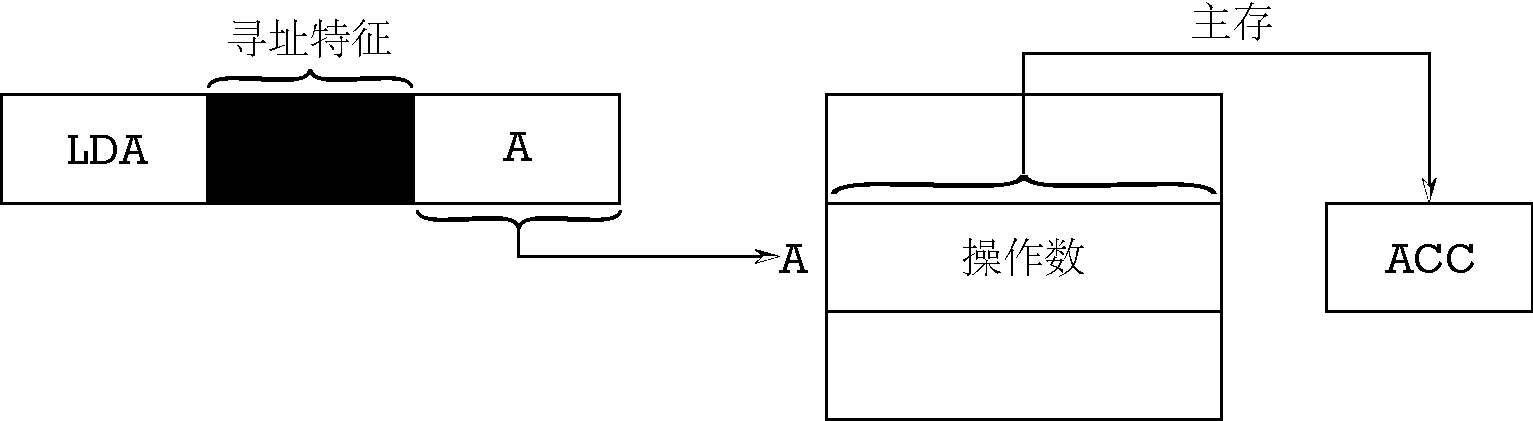
\includegraphics[scale=.4]{img/figure3.pdf}
\end{figure}
\item 间接寻址: 指令中的形式地址\verb|A|是真实地址的地址, 即\verb|(A)=EA|
\begin{figure}[H]
\centering
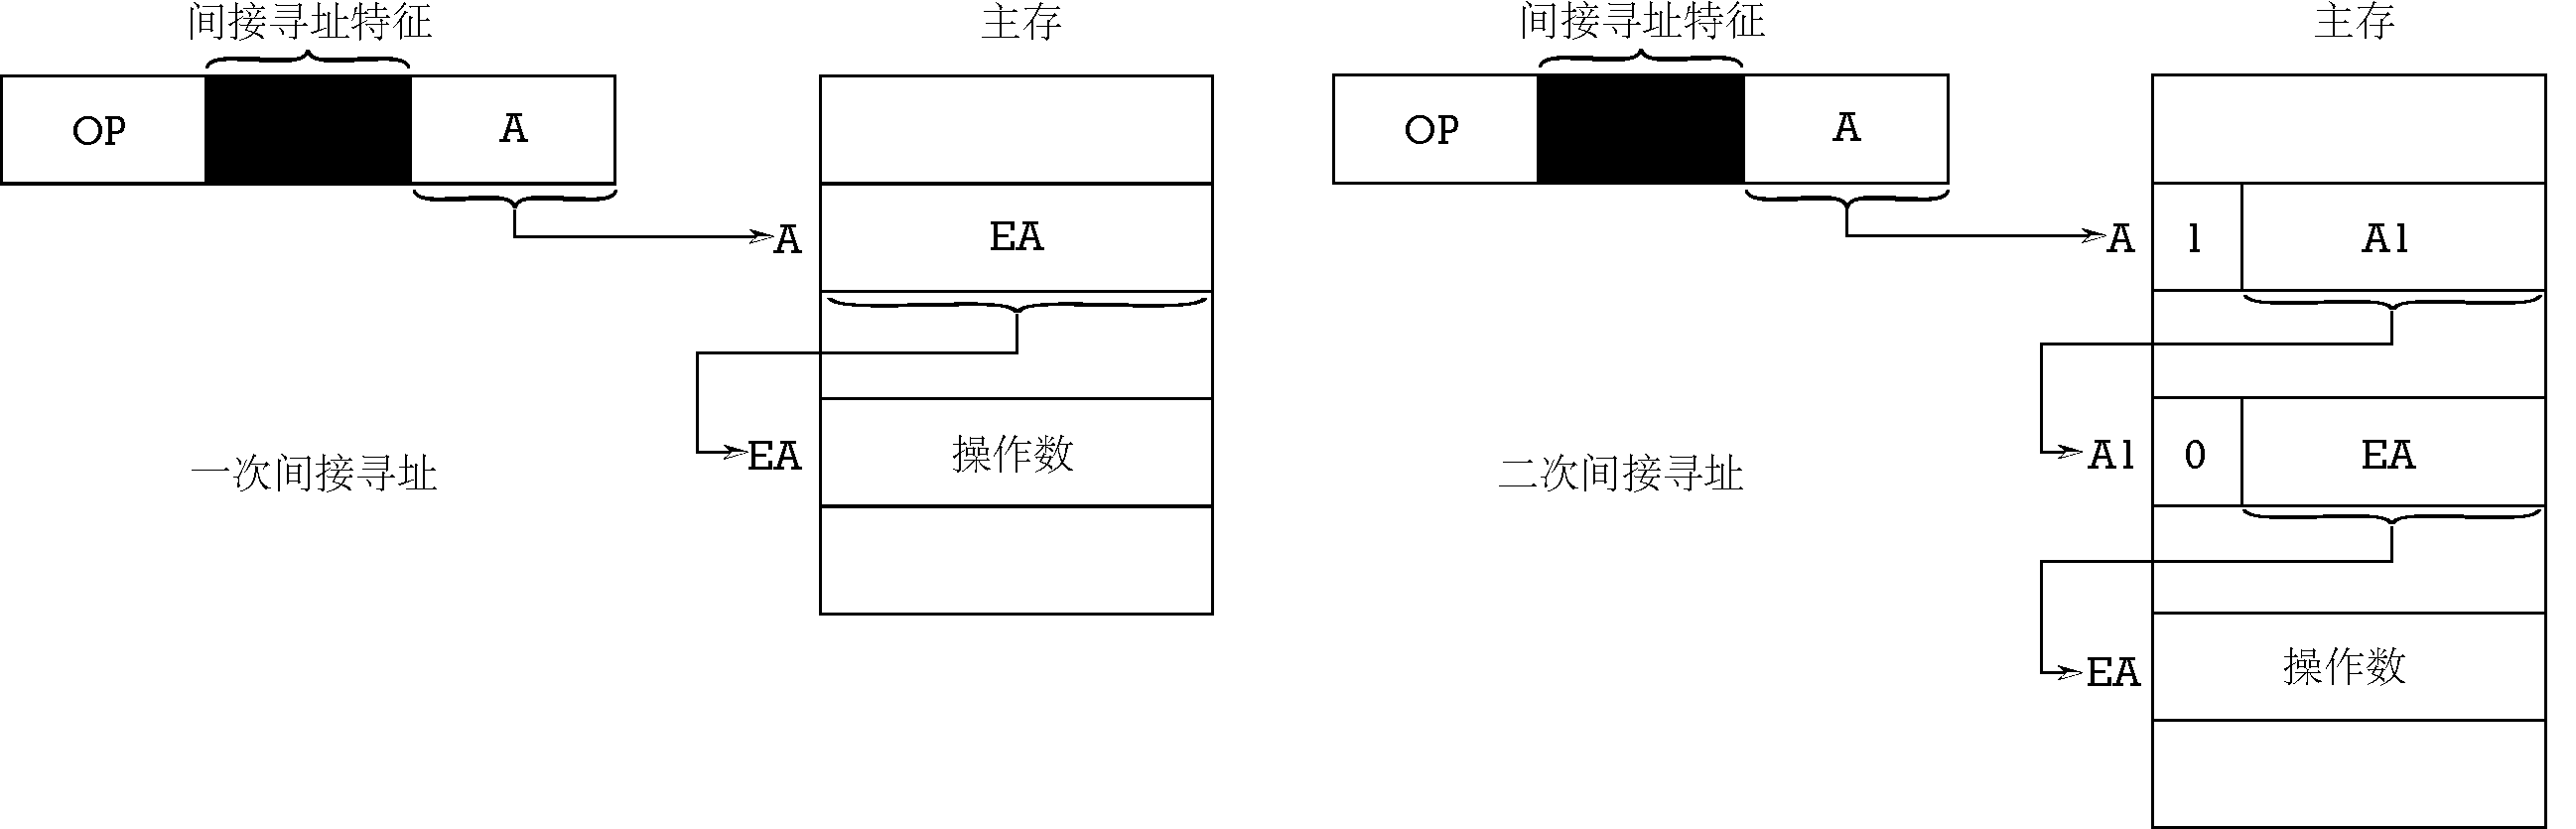
\includegraphics[scale=.4]{img/figure4.pdf}
\end{figure}
\item 寄存器寻址: 指令中的地址是寄存器号\verb|Ri|, 寄存器中存储了操作数, 即\verb|Ri=EA|
\begin{figure}[H]
\centering
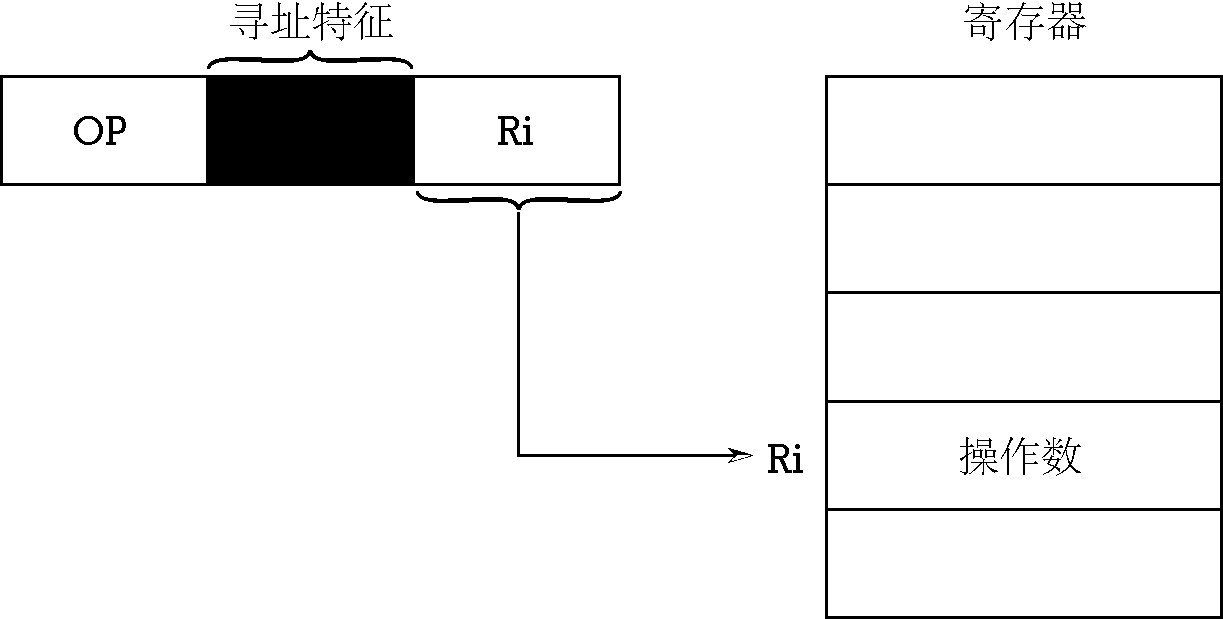
\includegraphics[scale=.4]{img/figure5.pdf}
\end{figure}
\item 寄存器间接寻址: 指令中的地址是寄存器号\verb|Ri|, 寄存器中存储了真实地址\verb|EA|, 即\verb|(Ri)=EA|
\begin{figure}[H]
\centering
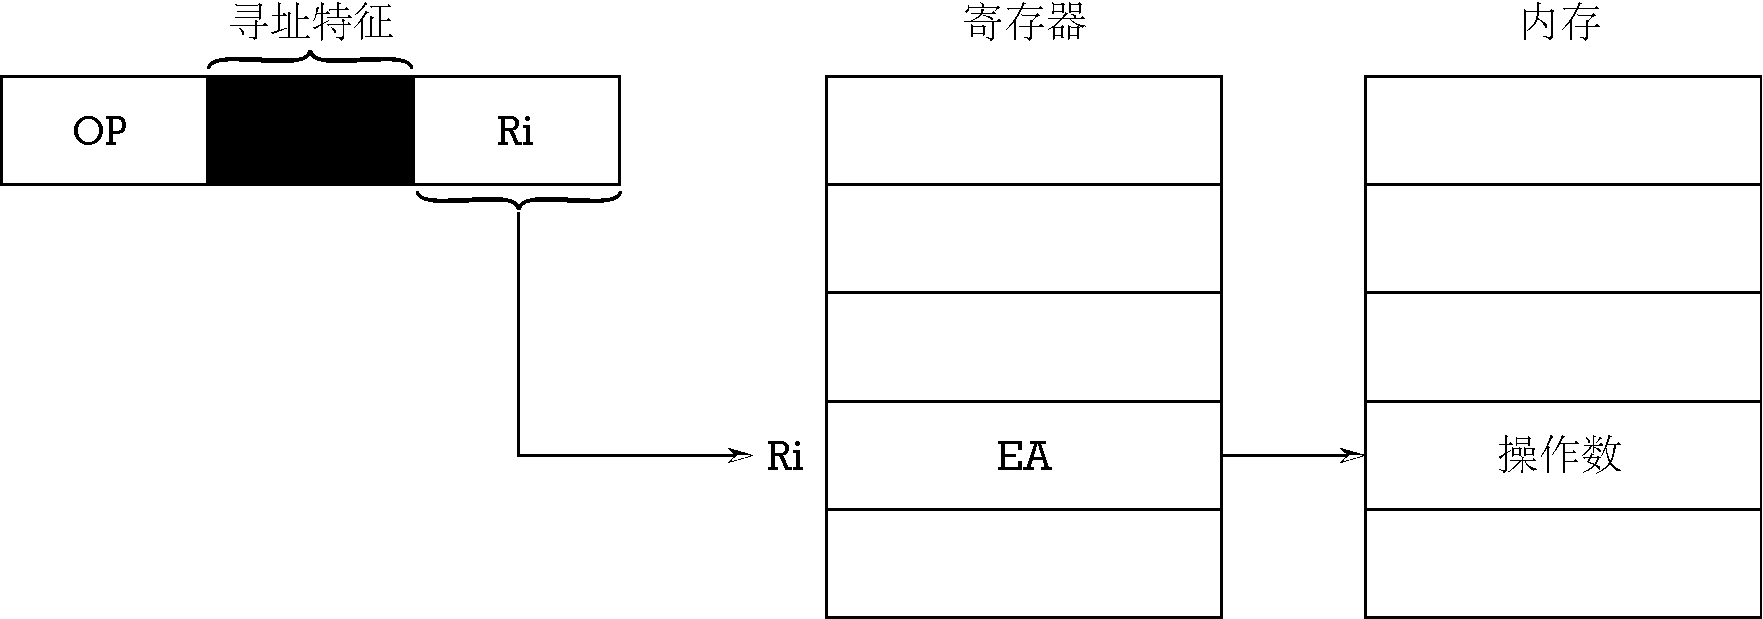
\includegraphics[scale=.4]{img/figure6.pdf}
\end{figure}
\item 相对寻址: 将程序计数器\verb|PC|的内容和指令中的形式地址\verb|A|相加得到真实地址\verb|EA|, 即\verb|(PC)+A=EA|
\begin{figure}[H]
\centering
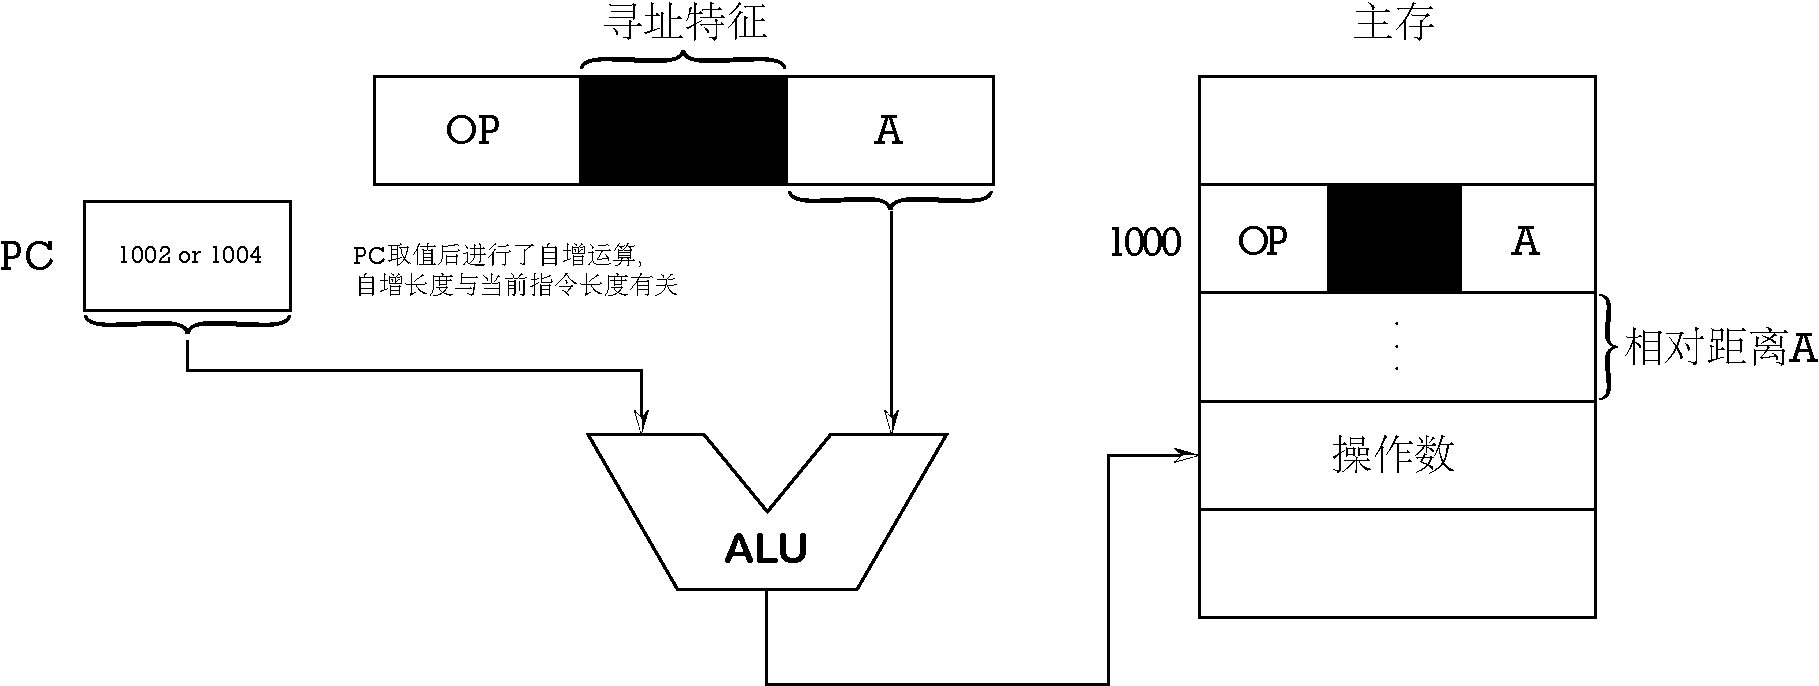
\includegraphics[scale=.4]{img/figure7}
\end{figure}
\item 基址寻址: 将基址寄存器\verb|BR|的内容和指令中的形式地址\verb|A|相加得到真实地址\verb|EA|, 即\verb|(BR)+A=EA|
\begin{figure}[H]
\centering
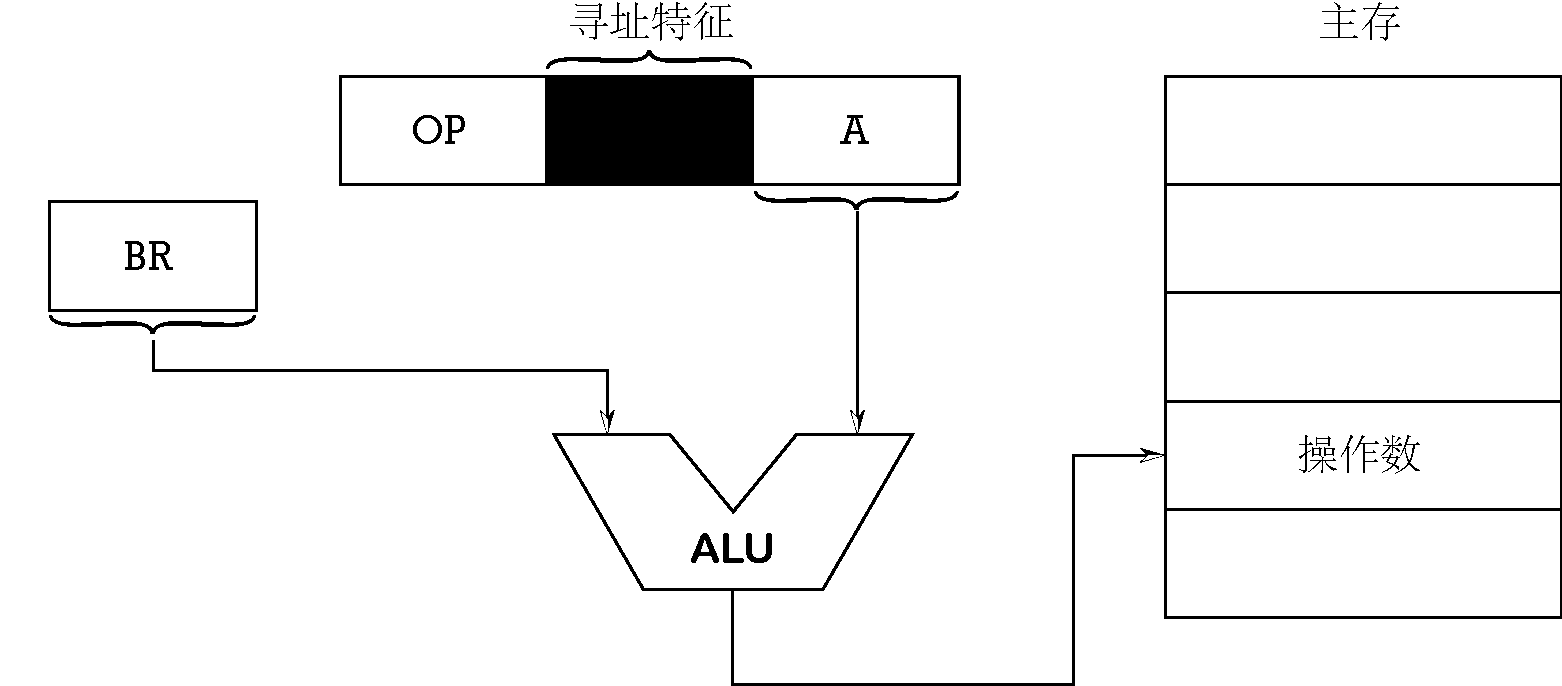
\includegraphics[scale=.4]{img/figure8}
\end{figure}
\end{enumerate}
\chapter{运算}
\section{进位计数制}
\subsection{进位计数法}
\verb|r|进制数, 每个数码位可能出现\verb|r|种字符, 逢\verb|r|进\verb|1|.
\subsection{不同进制数之间的转换}
\subsubsection{\texttt{r}进制数$ \rightarrow $十进制}
各数码位与位权的乘积之和, 全为\verb|1|的二进制转十进制: \verb|2^n-1|
\subsubsection{十进制$ \rightarrow $ \texttt{r}进制}
\begin{itemize}
\item 整数部分: 除基取余法, 先取得的``余''是整数的低位(除\verb|r|)
\item 小数部分: 乘基取整法, 先取得的``整''是消暑的高位(乘\verb|r|)
\end{itemize}
\subsubsection{二进制$ \leftrightarrow $八进制}
每三个二进制位对应一个八进制位
\subsubsection{二进制$ \leftrightarrow $十六进制}
每四个二进制位对应一个十六进制位
\section{定点数的表示}
\subsection{数的分类}
\begin{itemize}
\item 有符号数
\begin{itemize}
\item 定点数: 小数点位置固定的数
\begin{itemize}
\item 定点整数: 纯整数
\item 定点小数: 纯小数
\end{itemize}
\item 浮点数: 小数点位置不定的数(既有整数又有小数)
\end{itemize}
\item 无符号数(如地址)
\end{itemize}
\subsection{真值和机器数}
\begin{itemize}
\item 真值: 实际带正负号的数值(人类习惯的样子)
\item 机器数: 把正负号数字化的数(存到机器里的样子), 包括原码, 反码, 补码, 移码, 他们都是有符号数
\end{itemize}
\subsection{原码}
\begin{enumerate}
\item 含义 \par
用尾数表示真值的绝对值, 符号位``0/1''对应``正/负''. 若机器字长为\verb|n+1|位, 则尾数就占\verb|n|位.
\item 范围 \par
\verb|0|表示不唯一, (\verb|[+0]原=0,0000000,[-0]原=1,000000|), 范围为\verb|-2^n-1~2^n-1|, \verb|n|为尾数长度
\item 示例 \par
机器字长为\verb|8|位, 将真值\verb|x=-14|转换为原码: \verb|[x]原=1,0001110|(注意: 不足的机器字长要补\verb|0|)
\end{enumerate}
\subsection{反码}
\begin{enumerate}
\item 含义 \par
\begin{itemize}
\item 正数: 与原码相同
\item 负数: 符号位不变, 数值位取反
\end{itemize}
\item 范围 \par
\verb|0|表示方法不唯一, (\verb|[+0]反=0,0000000, [-0]反=1,1111111|), 范围为\verb|-2^n-1~2^n-1|, \verb|n|为尾数长度
\item 示例 \par
机器字长为\verb|8|位, 将真值\verb|x=-14|转换为反码: \verb|[x]反=1,1110001|
\end{enumerate}
\subsection{补码}
\begin{enumerate}
\item 含义 \par
先将原码转化为反码, 再将数值位\verb|+1|. \par 或者, 将原码直接转为补码: 从后往前, 遇到的第一个\verb|1|之前不变, 后面取反(符号位不变), 反过来补码转原码也是如此.
\item 范围 \par
\verb|0|的表示方法唯一, (\verb|[0]=0,0000000, 1,0000000用于表示-128|), 范围为\verb|-2^n~2^n-1|, \verb|n|为尾数长度
\item 示例 \par
机器字长为\verb|8|位, 将真值\verb|x=-14|转换为补码: 原码为\verb|[x]原=1,0001110|, 从右往左第一个\verb|1|不变, 左边取反, 得到补码\verb|[x]补=1,1110010|
\end{enumerate} \par 比较这两个数字的大小: \verb|1,1111111|和\verb|1,0000000|, 前者大, 因为前者转换为真值是\verb|1|, 而后者转化为真值为\verb|-128|
\subsection{移码}\label{移码}
移码与原码, 反码, 补码不同, 他是一种无符号数. \par 移码=真值+偏置值, 若机器字长为\verb|n+1|位, 则偏置值为\verb|+2^n|, 当偏置值为\verb|+128|的时候: 补码=补码的符号位取反. \par
偏置值可以取其他值, 如在\hyperref[IEEE 754]{\texttt{IEEE 754}}中, 单精度浮点数的偏移量为\verb|+127|, 即\verb|+01111111|.
\section{定点数的运算}
\subsection{移位运算} % TODO 移位运算的溢出问题
左移相当于\verb|*2|, 右移相当于\verb|/2|
\begin{itemize}
\item 逻辑移位: 无符号数, 当成正数, 补\verb|0|
\item 算术移位: 有符号数, 有正有负
\begin{itemize}
\item 正数: 符号位不参与移位, 原码, 反码, 补码数值位均补\verb|0|
\item 负数: 符号位不参与移位, 原码补\verb|0|, 反码补\verb|1|, 补码如果是左移, 补\verb|0|; 如果是右移, 补\verb|1|
\end{itemize}
\end{itemize} \par
左移: 若舍弃的位为\verb|1|, 将产生严重误差; \par 右移: 若舍弃的位为\verb|1|, 将丢失精度.
\subsection{加减运算}
\begin{itemize}
\item 原码的加减运算
\begin{itemize}
\item 加法运算
\begin{itemize}
\item 正+正: 绝对值做加法, 符号位为\verb|0|
\item 负+负: 绝对值做加法, 符号位为\verb|1|
\item 正+负: 绝对值大的减绝对值小的, 符号位同绝对值大的数
\item 负+正: 绝对值大的减绝对值小的, 符号位同绝对值大的数
\end{itemize}
\item 减法运算: 减数的符号位取反, 转变为加法
\end{itemize}
\item 补码的加减运算
\begin{itemize}
\item 加法运算: \verb|[A+B]补=[A]补+[B]补|
\item 减法运算: \verb|[A-B]补=[A]补+[-B]补|
\end{itemize}
\end{itemize}
\section{浮点数的表示和运算}
\subsection{浮点数的表示格式}
浮点数\verb|N=M*r^E|, 其中\verb|N|为浮点数, \verb|M|为尾数, \verb|E|为阶码, \verb|r|为基数, 二进制的话为\verb|2|, 上述数字均为十进制.
\begin{figure}[H]
\centering
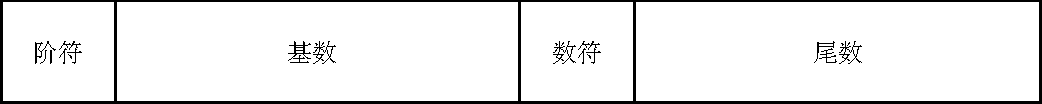
\includegraphics[scale=.7]{img/figure9.pdf}
\end{figure}
\subsection{浮点数的规格化}
规格化浮点数: 规定原码尾数的最高位一定要是个1$ \Leftrightarrow $ \texttt{|M|}属于\verb|[0.5,1]|, 所以衍生出以下两种规范化的方法:
\begin{itemize}
\item 左规: 说明\texttt{M<1/2}, 太小, 需要扩大, 左移\verb|1|位将尾数的数值位扩大到原来的\verb|2|倍, 同时阶码减\verb|1|
\item 右规: 说明\texttt{M>1}, 太大, 需要缩小, 右移\verb|1|位将尾数的数值位缩小到原来的\verb|1/2|倍, 同时阶码加\verb|1|
\end{itemize}\par
尾数可以用原码或者是补码表示, 所以上述左规和右规可以分别用于原码或者补码的规格化:
\begin{itemize}
\item 原码: 尾数最高位为\verb|1|
\begin{itemize}
\item 尾数为正数: 通过左规和右规得到的标准形式应该是\verb|0.1XXXXXXXX|
\item 尾数为负数: 通过左规和右规得到的标准形式应该是\verb|1.1XXXXXXXX|
\end{itemize}\par
注意, 上面尾数可以等于\verb|0.5|或者是\verb|-0.5|, 只要是\verb|0.1000000...|和\verb|1.1000000...|即可. 但是做不到等于\verb|1|或者\verb|-1|. 此外, 他们的数值位第一位都是\verb|1|, 所以在\hyperref[IEEE 754]{\texttt{IEEE 754}}中, 数值位的第一位可以默认省略.
\item 补码: 尾数最高位与符号位相反
\begin{itemize}
\item 尾数为正数: 通过左规和右规得到的标准形式应该是\verb|0.1XXXXXXXXX|
\item 尾数为负数: 通过左规和右规得到的标准形式应该是\verb|1.0XXXXXXXXX|
\end{itemize}
\end{itemize}
\subsection{\texttt{IEEE 754}标准}\label{IEEE 754} % TODO 阶码中的0和1有特殊用途, 以及IEEE表示范围
\begin{figure}[H]
\centering
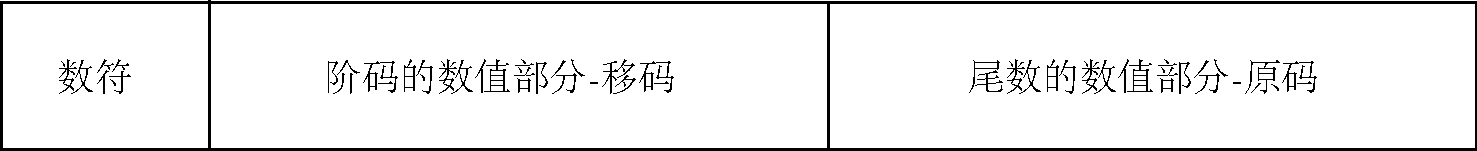
\includegraphics[scale=.5]{img/figure10.pdf}
\end{figure}
\subsubsection{阶码}
阶码用移码表示, 单精度浮点数下长度为\verb|8|位. \par
\hyperref[移码]{移码}是一种无符号数, 由于移码=真值+偏置值, 加完之后大于等于\verb|0|, 所以阶码没有符号位. 偏置值和数的类型有关, 单精度浮点数的偏置值为\verb|+127|, 双精度浮点数的偏置值为\verb|+1023|.
\subsubsection{尾数}
尾数用原码表示, 单精度浮点数下长度为\verb|23|位. \par
尾数是一种有符号数, 他的符号放在开头, 数值部分放在末尾. 通过规格化后, 数值部分默认隐藏首位\verb|1|, 所以单精度浮点数下实际能表示的数值位有\verb|24|位.
\subsubsection{举例}
以\verb|-1.75*2^(-3)|为例: \par
\begin{itemize}
\item 数符: 由于是负数, 所以是\verb|1|. \par
\item 尾数的数值部分: 十进制下是\verb|1.75>1|, 故需要右归, 尾数的数值部分右移\verb|1|位, 阶码需要加\verb|1|, 得到尾数的数值位为\verb|0.875|即\verb|1110000...(共24位)|, 阶码为\verb|-2|. 由于尾数的数值位的首位\verb|1|可以省略, 所以最终尾数的数值位为\verb|110000...(共23位)|. \par
\item 阶码: 经过上述规格化后, 阶码为\verb|-2|, 加上偏置值\verb|+127|, 得到移码十进制下为\verb|+125|, 转换为二进制为\verb|01111101|. \par
\end{itemize}
综上所述, 我们得到的\verb|IEEE 754|下的表示为: \verb|1,01111101,110000...(共23位)|.
\subsection{浮点数的加减运算}
我们通常在十进制下做浮点数的加减运算.
\subsubsection{步骤}
\begin{enumerate}
\item 对阶: 保持阶数一致, 小阶数向大阶数对齐
\item 尾数相加/减
\item 规格化, 保证尾数\verb|M|属于\verb|[0.5,1]|
\end{enumerate}
\subsubsection{举例}
实现\verb|0.75*2^4+1.5*2^3|:
\begin{enumerate}
\item 对阶: 小阶$ \rightarrow $大阶, \verb|1.5*2^3|$ \rightarrow $\verb|0.75*2^4|
\item 加减: \verb|0.75*2^4+0.75*2^4=1.5*2^4|
\item 规格化: \verb|1.5*2^4|$ \rightarrow $\verb|0.75*2^5|
\end{enumerate}
\chapter{存储器}
\section{存储器的层次}
\begin{figure}[H]
\centering
\begin{subfigure}{.48\textwidth}
\centering
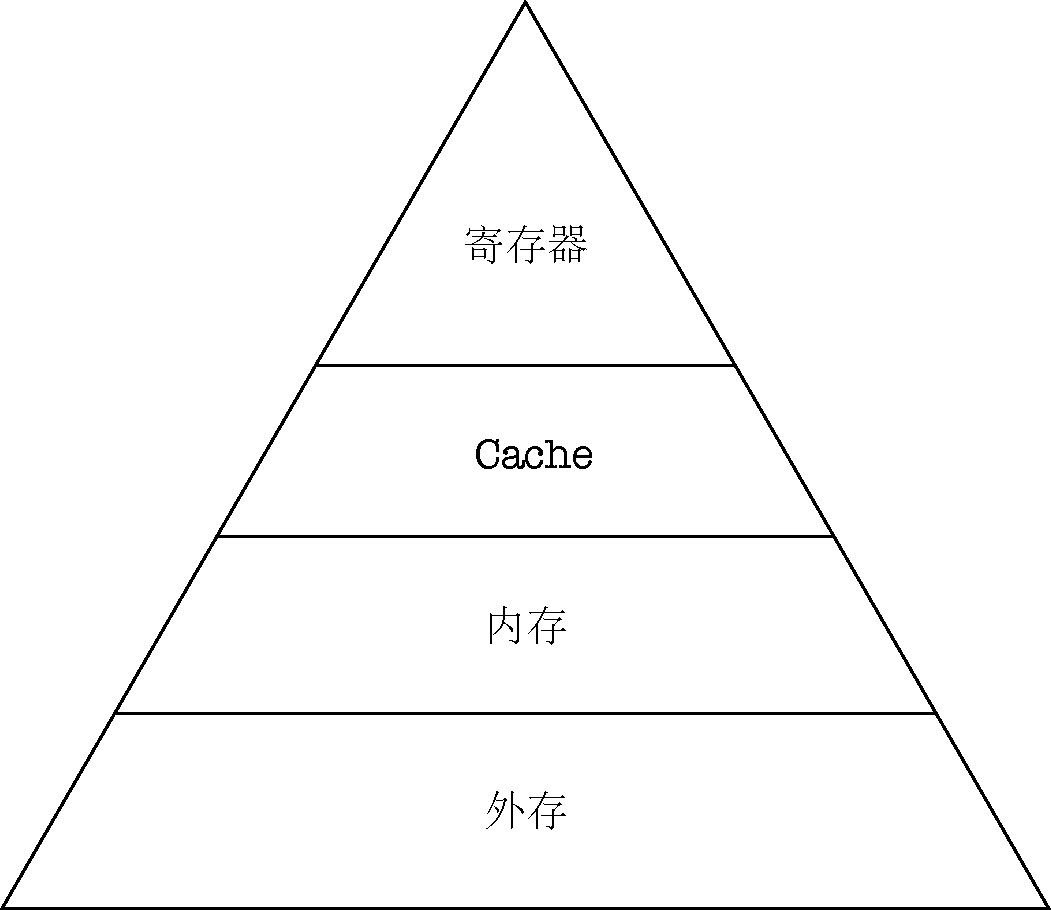
\includegraphics[scale=.3]{img/figure11.pdf}
\caption{多级存储器结构}
\end{subfigure}
\begin{subfigure}{.48\textwidth}
\centering
\flushleft
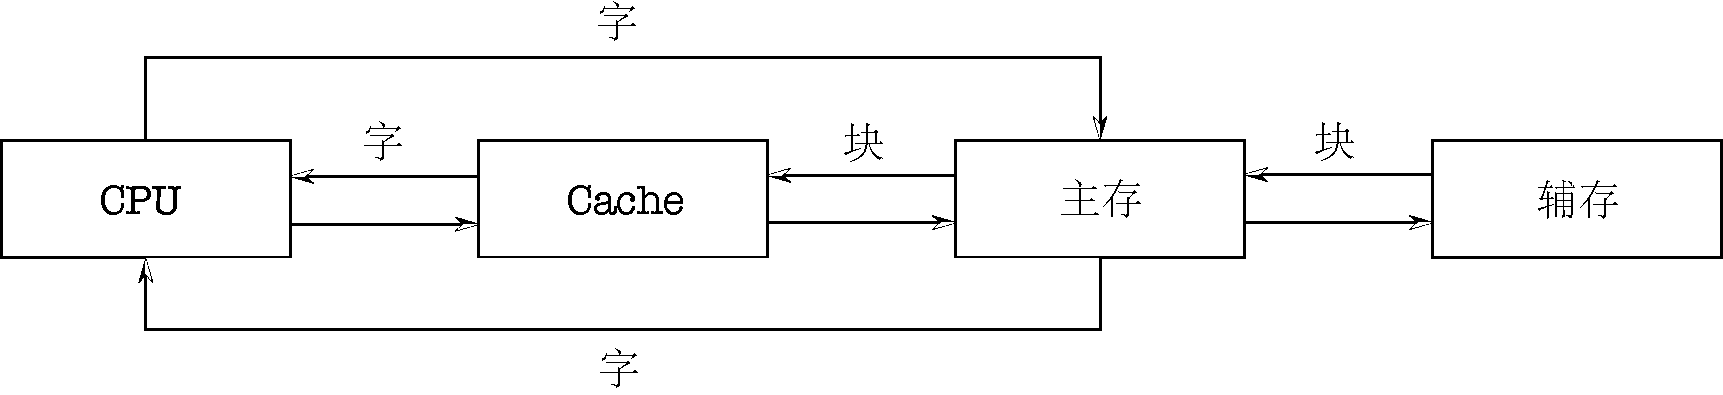
\includegraphics[scale=.3]{img/figure12.pdf}
\caption{存储器之间的数据交换}
\end{subfigure}
\end{figure}
这就是存储器的层次结构. 在\verb|pyramid|的越上层, 价格越高, 速度越快, 容量越小. 要注意的是, \verb|Cache|和主存之间的数据交换是由硬件完成的, 对所有程序员透明. 主存和辅存之间的数据交换是由硬件和操作系统共同完成的. 对应用程序员透明.
\section{存储器的分类}
\begin{itemize}
\item 按层次分类
\begin{itemize}
\item 主存储器: 简称主存, 或者内存. 可以直接和\verb|Cache|交互
\item 辅助存储器: 简称辅存, 或者外存. 是主存的后援存储器
\item 高速缓冲存储器: 简称\verb|Cache|. 放在\verb|CPU|中
\end{itemize}
\item 按存取分类
\begin{itemize}
\item 随机存储器: \verb|RAM|, 可读可写, 存取时间和物理位置无关, 断电丢失数据
\begin{itemize}
\item 静态随机存储器: \verb|SRAM|, 双稳态触发器, 用于\verb|Cache|
\item 动态最急存储器: \verb|DRAM|, 栅极电容, 用于内存
\end{itemize}
\item 只读存储器: \verb|ROM|, 只读, 存取时间和物理位置无关, 断电不丢失数据
\item 串行访问存储器: 存储时间和物理位置有关, 如顺序存取存储器(磁带)与直接存取存储器(磁盘,光盘)
\end{itemize}
\item 按介质分类
分为: 磁表面存储器(磁盘,磁带), 磁芯存储器, 半导体存储器(MOS型存储器,双极型存储器)和光存储器(光盘)
\item 按可保存性分类
\begin{itemize}
\item 易失存储器: 断电后, 存储信息消失. 如: \verb|RAM|
\item 非易失存储器: 断电后, 存储信息依然保持, 如: \verb|ROM|
\item 破坏性读出: 某个存储单元被读出时, 原存储器信息被破坏
\item 非破坏性读出: 某个存储单元被读出时, 原存储器信息不会被破坏
\end{itemize}
\end{itemize}
\section{\texttt{Cache}}
\verb|Cache|是由\verb|SRAM|构成的, 在\verb|CPU|中的一种存储器.
\subsection{基本原理}
操作系统为了缓和\verb|CPU|和主存之间的速度矛盾, 将某些主存块放到了\verb|Cache|中, 而这个步骤是基于局部性原理:
\begin{itemize}
\item 时间局部性: 现在访问的地址, 不久之后也很可能再次被访问
\item 空间局部性: 现在访问的地址, 其附近的地址也很可能即将被访问
\end{itemize}
\subsection{主存到\texttt{Cache}的映射}
\verb|Cache|被分成与主存的页框大小一致的\verb|Cache|块(或称Cache行), 两者之间以块为单位进行数据交换. 下面解释了内存中的块应该放在\verb|Cache|中的哪个位置:
\subsubsection{全相联映射}
主存的块可以装入\verb|Cache|的任何块, 没有公式. 相应的地址结构为:
\begin{figure}[H]
\centering
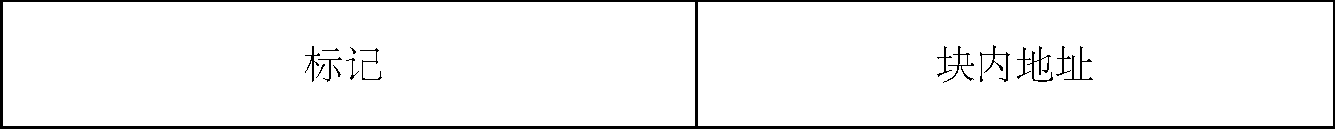
\includegraphics[scale=.5]{img/figure13.pdf}
\end{figure}
\subsubsection{直接映射}
主存中的块必须放入下面公式的指定\verb|Cache|块:
\begin{center}
\verb|j = i mod 2^c, 其中j为Cache块号, i为主存块号, 2^c为Cache的总块数|
\end{center} \par
\par 从上面的映射关系可以看出, 主存块号的低\verb|c|位正是它要装入的\verb|Cache|行号. 若主存中用\verb|m|位表示块号, 则标记(有效位+内存地址高位)共\verb|m-c|位, \verb|Cache|块号共\verb|c|位, 相应的地址结构为:
\begin{figure}[H]
\centering
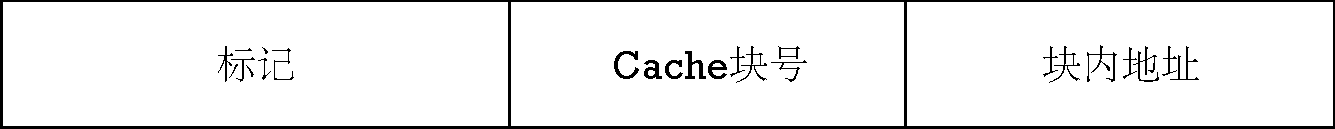
\includegraphics[scale=.5]{img/figure15.pdf}
\end{figure}\par
\subsubsection{组相联映射}
将\verb|Cache|分成大小相等的组, 主存的一个数据块可以装入一组内的任意位置, 即组间采取直接映射, 组内采取全相联映射, 内存块可以放在下面公式指定的\verb|Cache|\textbf{组}中:
\begin{center}
\verb|j = i mod Q, 其中j为Cache块号, i为主存块号, Q为组数|
\end{center}\par 
与直接映射相似, 主存块号的低位用来表示组号, 内存块号的高位和有效位用来表示标记, 相应的地址结构为:
\begin{figure}[H]
\centering
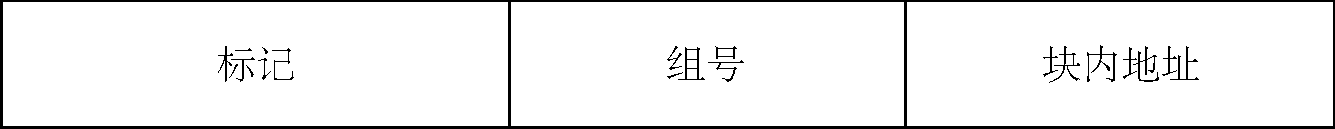
\includegraphics[scale=.5]{img/figure14.pdf}
\end{figure}
根据上述的地址结构, 我们应该可以推断出\verb|CPU|的访存过程:
\begin{figure}[H]
\centering
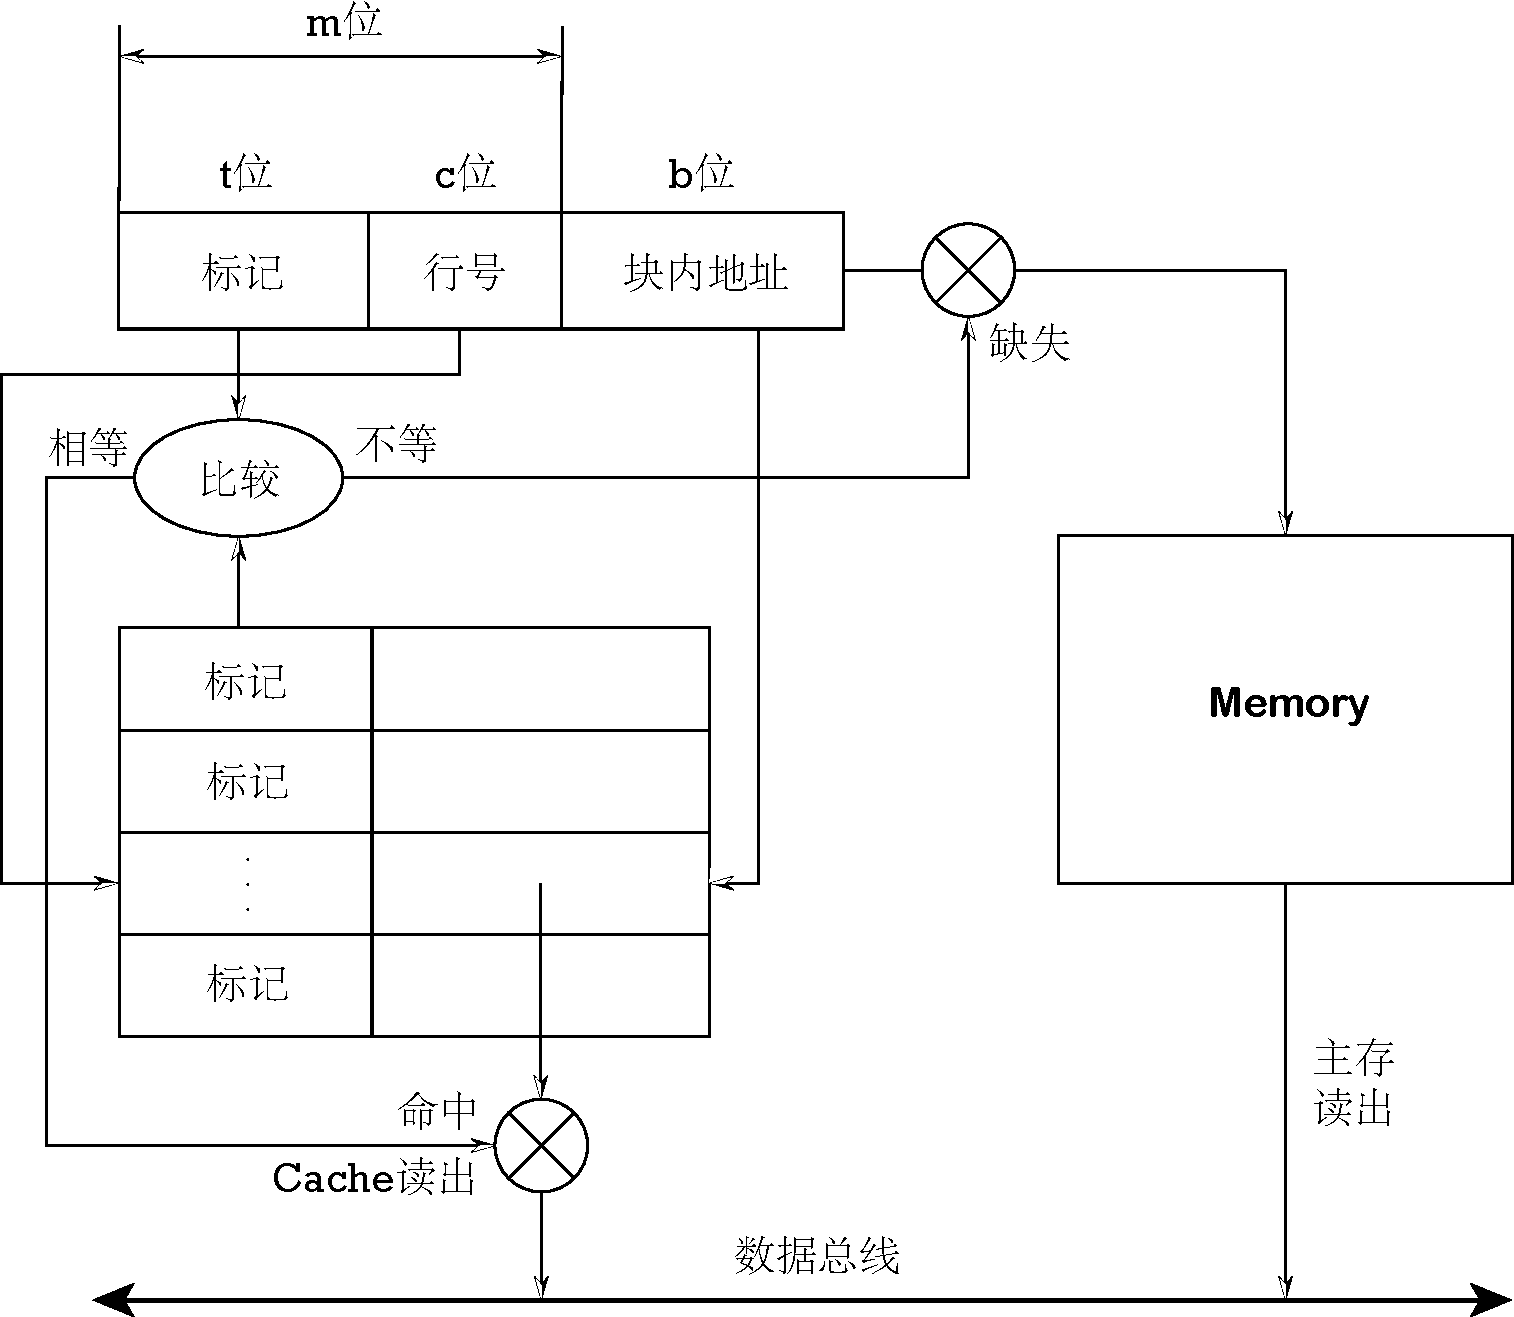
\includegraphics[scale=.4]{img/figure16.pdf}
\caption*{直接映射}
\end{figure}\par
上图为直接映射方式, 全相联映射中没有组,行号,内存地址高位低位的概念, 他的标记就是有效位+内存块号. 组相联映射是一种介于全相联映射和直接映射之间的一种映射.
\subsection{替换算法}
由于\verb|Cache|的空间通常很小, 所以用不到的\verb|Cache|块就要及时换出, 下面说明上述三种映射中替换算法要解决的问题:
\begin{itemize}
\item 全相联映射 \par \verb|Cache|满了才需要替换, 需要在全局选择替换哪一块
\item 直接映射 \par 如果对应位置非空, 则毫无选择地直接替换, 无需考虑替换算法
\item 组相联映射 \par 分组内满了才需要替换, 需要在分组内选择替换哪一块
\end{itemize}
\subsubsection{随机算法(\texttt{RAND})}
若\verb|Cache|已满, 则随机选择一块替换. \par
实现简单, 但是完全没有考虑局部性原理. 命中率低, 实际效果很不稳定.
\subsubsection{先进先出算法(\texttt{FIFO})}
若\verb|Cache|已满, 则替换最先被调入\verb|Cache|的块. \par
实现简单, 也是完全没有考虑局部性原理, 会出现抖动现象: 频繁的换入换出现象
\subsubsection{近期最少使用算法(\texttt{LRU})}
为每个\verb|Cache|设置一个``计数器'', 用于记录每个\verb|Cache|块已经多久没有被访问了, 当\verb|Cache|满后替换``计数器''最大的. \par
\begin{enumerate}
\item 命中 \par 命中行计数器清零, 比其低的计数器加\verb|1|, 其余不变
\item 未命中
\begin{enumerate}
\item 有空闲行 \par 空闲行计数器清零, 其余非空闲行加\verb|1|
\item 无空闲行 \par 计数器值最大行的信息块被淘汰, 新装行的块的计数器清零, 其余全加\verb|1|
\end{enumerate}
\end{enumerate}\par
该算法基于局部性原理, 运行效果优秀, \verb|Cache|命中率高.
\subsubsection{最不经常使用算法\texttt{LFU}}
为每个\verb|Cache|设置一个``计数器'', 用于记录每个\verb|Cache|块被访问过几次, 当\verb|Cache|满后替换``计数器''最小的. \par
新调入的块计数器\verb|=0|, 之后每一次被访问计数器\verb|+1|, 需要替换的时候, 选择计数器最小的一行(若相同, 选择行号更小的一行). \par
最被经常访问的主存块在未来不一定会用得到, 并没有很好的遵循局部性原理, 实际效果不如\verb|LRU|.
\subsection{\texttt{Cache}写策略}
由于\verb|CPU|在访存的时候会优先访问\verb|Cache|, 假设这次的命令是要到某个块里修改数据, 那么就有两种情况, 即``写命中''(要写的块在\verb|Cache|中)和``写不命中''(要写的块不在\verb|Cache|中), 他们均会造成内存和\verb|Cache|的数据不一致性, 下面的方法能解决这个问题:
\begin{itemize}
\item 写命中
\begin{itemize}
\item 写回法
\item 全写法
\end{itemize}
\item 写不命中
\begin{itemize}
\item 写分配法
\item 非写分配法
\end{itemize}
\end{itemize}
\subsubsection{写回法}
适用于写命中. 只修改\verb|Cache|中的内容, 而不立即写入主存, 只有在此块被换出的时候再写回主存. \par
减少了访问次数, 但是存在数据不一致的隐患.
\subsubsection{全写法(写直达法)}
适用于写命中. 同时修改\verb|Cache|中的数据和主存中的内容, 一般使用写缓冲的方法, 创建一个队列, 慢慢地写回主存. \par 
访存次数增加, 速度变慢, 但能保证数据的一致性. 如果使用写缓冲, 若写操作很频繁, 会导致写缓冲饱和而阻塞.
\subsubsection{写分配法}
适用于写不命中. 把主存中的块调入\verb|Cache|, 在\verb|Cache|中修改. 搭配写回法使用.
\subsubsection{非写分配法}
适用于写不命中. 只写入主存, 不调入\verb|Cache|. 搭配全写法使用.
\subsection{多级\texttt{Cache}}
各级\verb|Cache|之间使用的是``全写法+非写分配法'', \verb|Cache|-主存之间使用的是``写回法+写分配法''.
\chapter{处理器}
\section{处理器的结构}
\verb|CPU|由控制器和运算器组成:
\begin{figure}[H]
\centering
\begin{subfigure}{.48\textwidth}
\centering
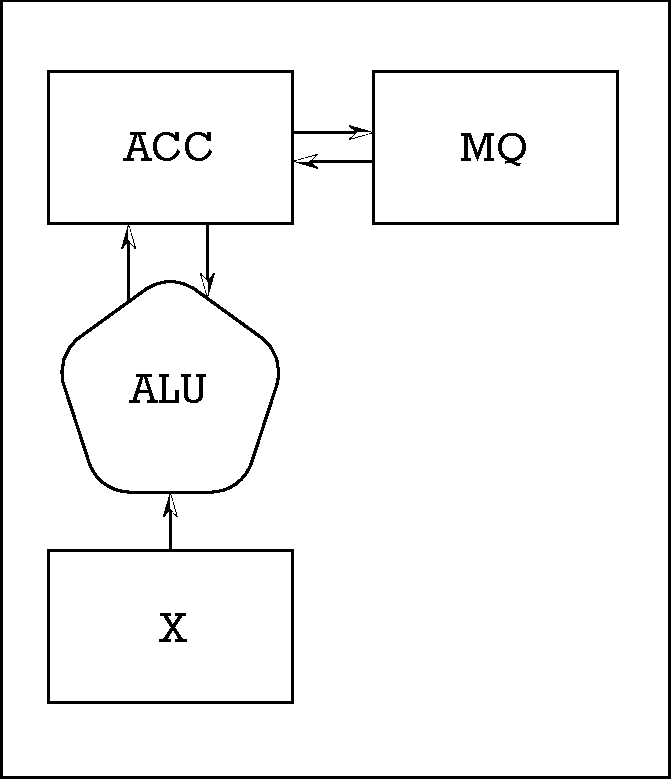
\includegraphics[scale=.5]{img/figure19.pdf}
\caption{运算器}
\end{subfigure}
\begin{subfigure}{.48\textwidth}
\centering
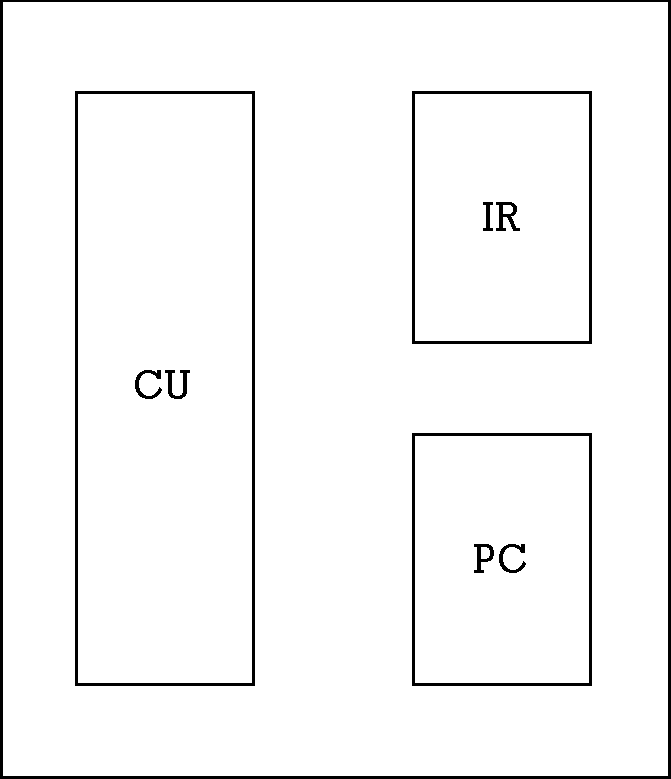
\includegraphics[scale=.5]{img/figure20.pdf}
\caption{控制器}
\end{subfigure}
\end{figure}
\subsection{控制器}
控制器内有三个重要的部件:
\begin{itemize}
\item \verb|CU|: \verb|Control Unit|, 分析指令, 给出控制信号
\item \verb|IR|: \verb|Instruction Registor|, 存放当前指令
\item \verb|PC|: \verb|Program Counter|, 存放下一条指令的地址, 有自动加\verb|1|的功能
\end{itemize}\par
那么, 控制器能实现什么功能呢?
\begin{itemize}
\item 取指令
\item 分析指令
\item 执行指令, 发出各种操作命令
\item 控制程序输入及结果的输出
\item 总线管理
\item 处理异常情况和特殊请求
\end{itemize}
\subsection{运算器}
运算器内有四个重要的部件:
\begin{itemize}
\item \verb|ACC|: 累加器, 用于存放被操作数, 或者运算结果
\item \verb|MQ|: 乘商寄存器, 在乘, 除运算的时候, 用于存放操作数或者运算结果
\item \verb|X|: 通用的操作数寄存器, 用于存放操作数
\item \verb|ALU|: 算术逻辑单元, 通过内部复杂的电路实现算术运算, 逻辑运算
\end{itemize}
运算器的功能, 顾名思义, 实现算术和逻辑运算.
\section{指令周期}
\verb|CPU|从主存中取出并执行一条指令的时间称为指令周期. 不同指令的指令周期可能不同. 指令周期用若干的机器周期表示, 一个机器周期又包含若干时钟周期(节拍).\par 根据机器周期内的节拍数是否相等, 可以拆分为:
\begin{figure}[H]
\centering
\begin{subfigure}{.48\textwidth}
\centering
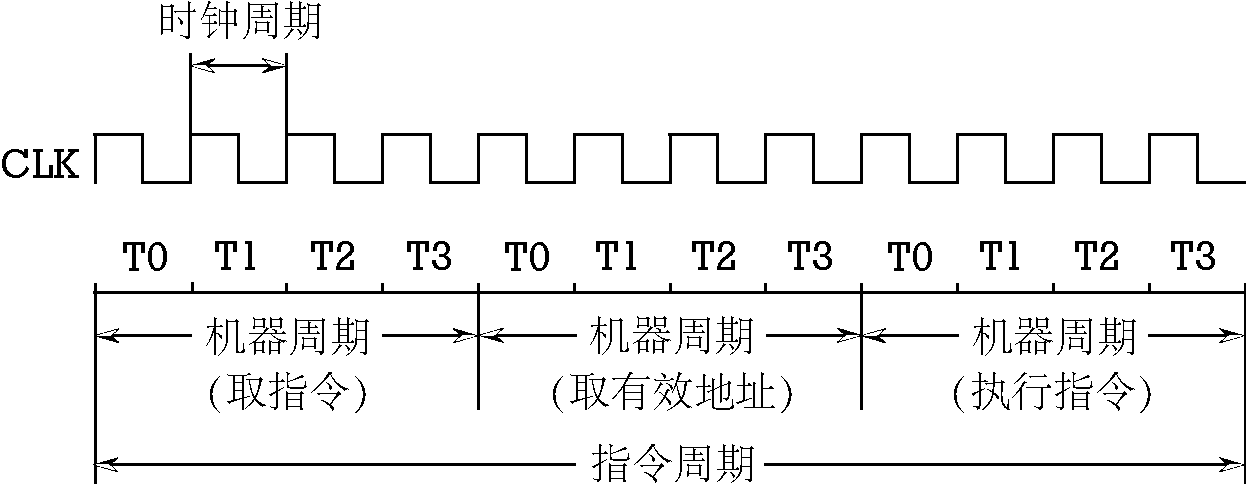
\includegraphics[scale=.4]{img/figure21.pdf}
\caption{定长机器周期}
\end{subfigure}
\begin{subfigure}{.48\textwidth}
\centering
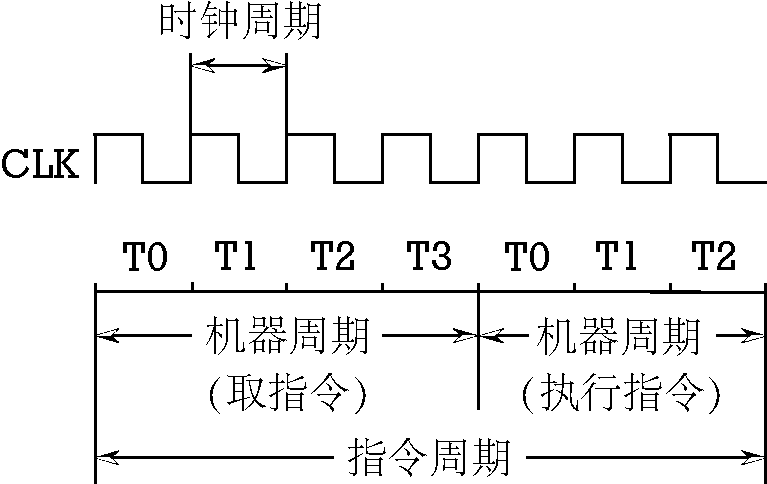
\includegraphics[scale=.4]{img/figure22.pdf}
\caption{不定长机器周期}
\end{subfigure}
\end{figure}
对于无条件转移指令\verb|j|, 在取值令完成后无需访存, 所以只包含取值周期和执行周期(都属于机器周期). \par
对于间接寻址指令, 在取指令完成后仍需访存, 因为取指令阶段取的是指令, 要根据这个指令访存取出有效地址, 所以还包括间址周期. \par
\verb|CPU|在每条指令结束之前, 都要发中断查询信号, 若有中断请求, 则\verb|CPU|进入中断响应阶段, 所以还包括中断周期. \par
综上所述, 一个一般的指令为:
\begin{figure}[H]
\centering
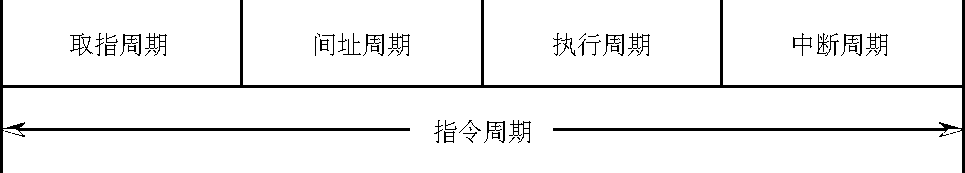
\includegraphics[scale=.6]{img/figure23.pdf}
\end{figure}
四个周期的工作:
\begin{itemize}
\item 取指周期: 取出并分析指令
\item 间址周期: 取有效地址
\item 执行周期: 取操作数, 并执行指令
\item 中断周期: 保存程序断点
\end{itemize}
\section{\texttt{MIPS}指令体系}
\subsection{一个基本的\texttt{MIPS}实现}
\begin{figure}[H]
\centering
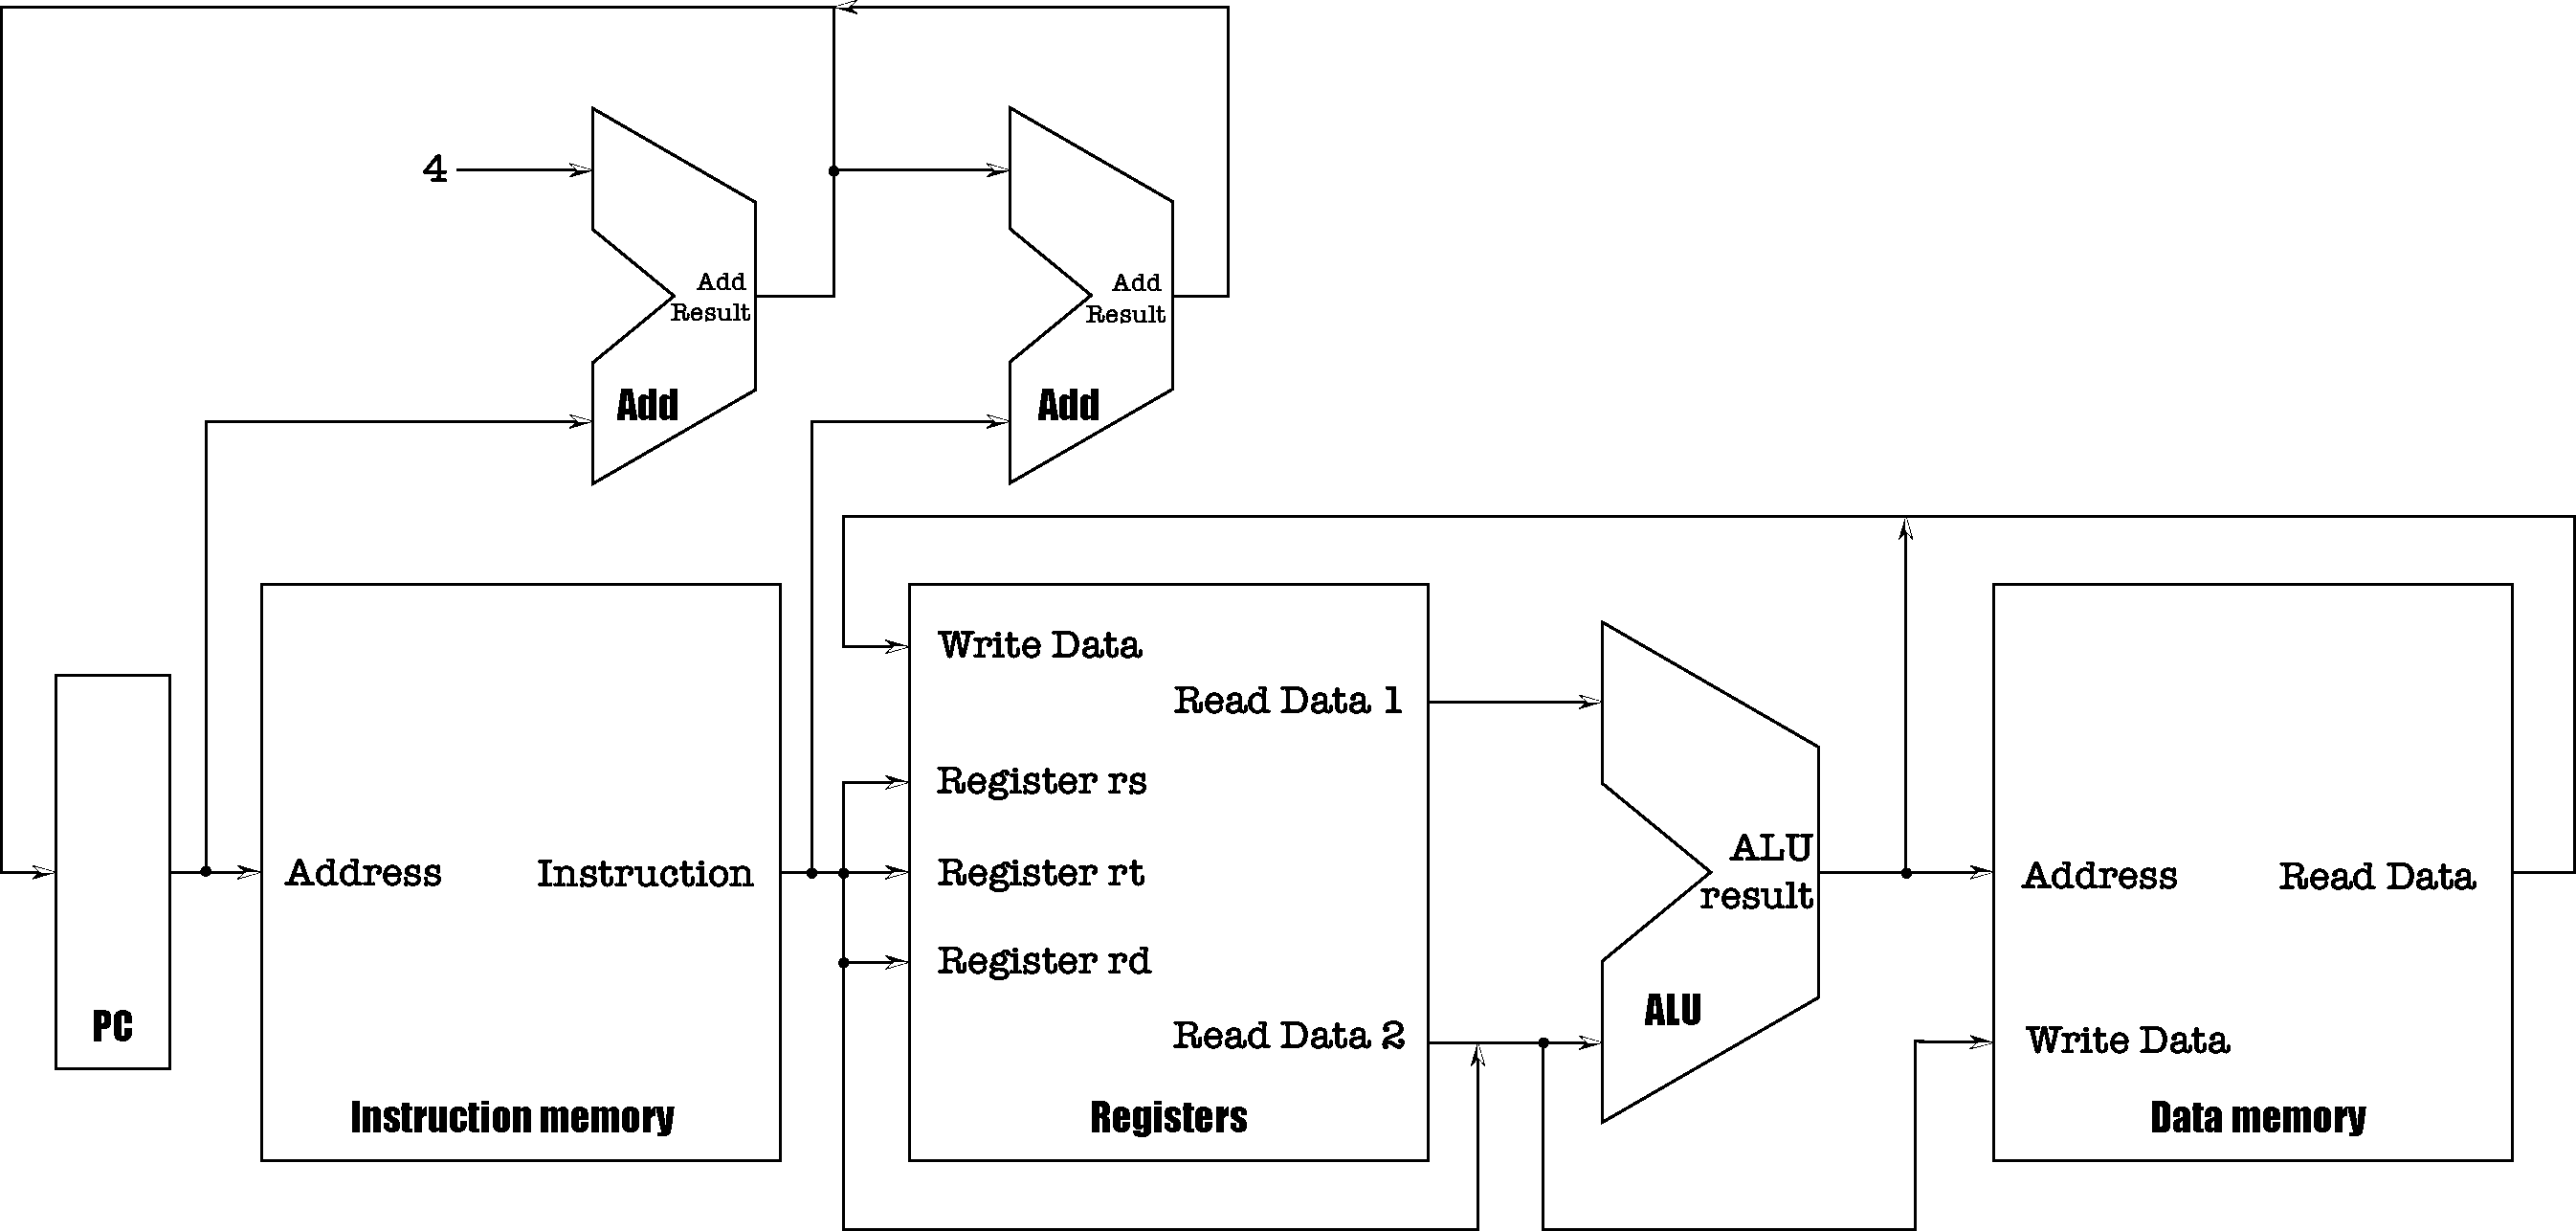
\includegraphics[scale=.3]{img/figure24.pdf}
\end{figure}
\subsubsection{\texttt{MIPS}子集基本实现(不包含选择器和控制器)}
\begin{enumerate}
\item \texttt{lw}操作 \par
我们以\verb|lw $t0, 32($s3)|为例, 首先, 将上述指令转化为十进制的样式:
\begin{table}[H]
\centering
\begin{tabularx}{\textwidth}{|Z|Z|Z|Z|}
\hline
\verb|35(op)| & \verb|19(rs)| & \verb|8(rt)| & \verb|32(Address)| \\
\hline
\end{tabularx}
\end{table}
然后, 将数据流在电路图中表示:
\begin{figure}[H]
\centering
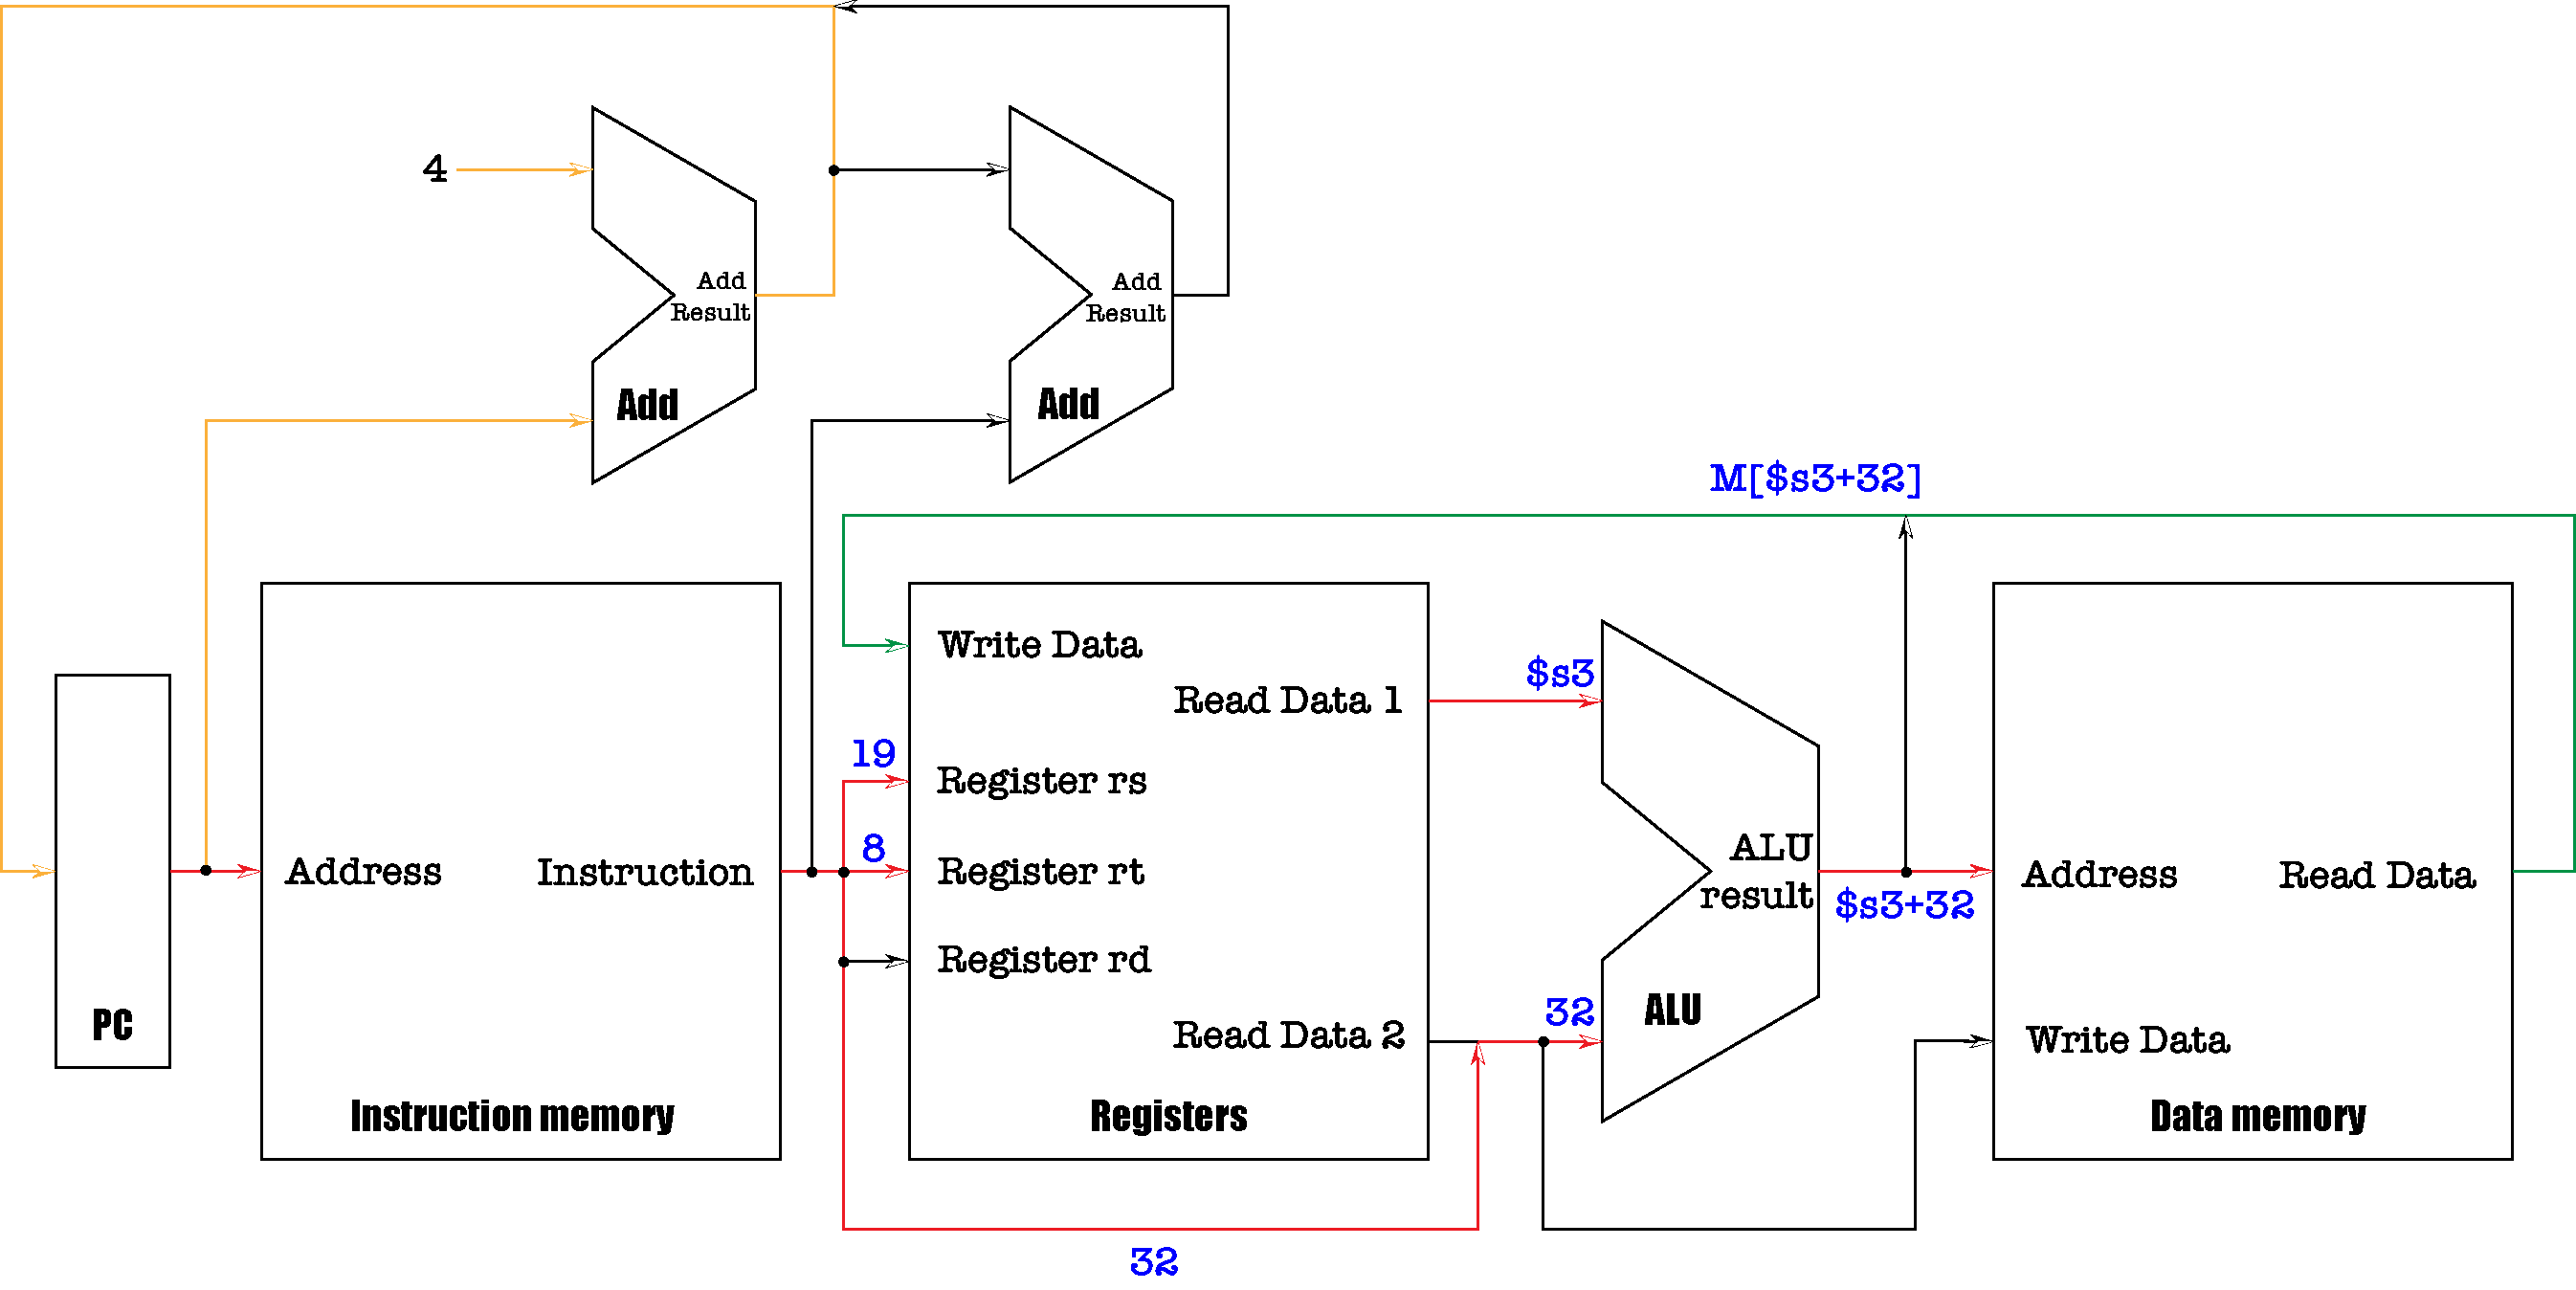
\includegraphics[scale=.3]{img/figure26.pdf}
\end{figure}
上图表示\verb|lw $t0, 32($s3)|指令执行的\textcolor{myred}{源数据流向}, \textcolor{mygreen}{结果流向}, \textcolor{myyellow}{\texttt{PC}改变}.
\item \texttt{sw}操作 \par
我们以\verb|sw $t0, 32($s3)|为例, 首先, 将上述指令转化为十进制的样式:
\begin{table}[H]
\centering
\begin{tabularx}{\textwidth}{|Z|Z|Z|Z|}
\hline
\verb|43(op)| & \verb|19(rs)| & \verb|8(rt)| & \verb|32(Address)| \\
\hline
\end{tabularx}
\end{table}
然后, 将数据流在电路图中表示:
\begin{figure}[H]
\centering
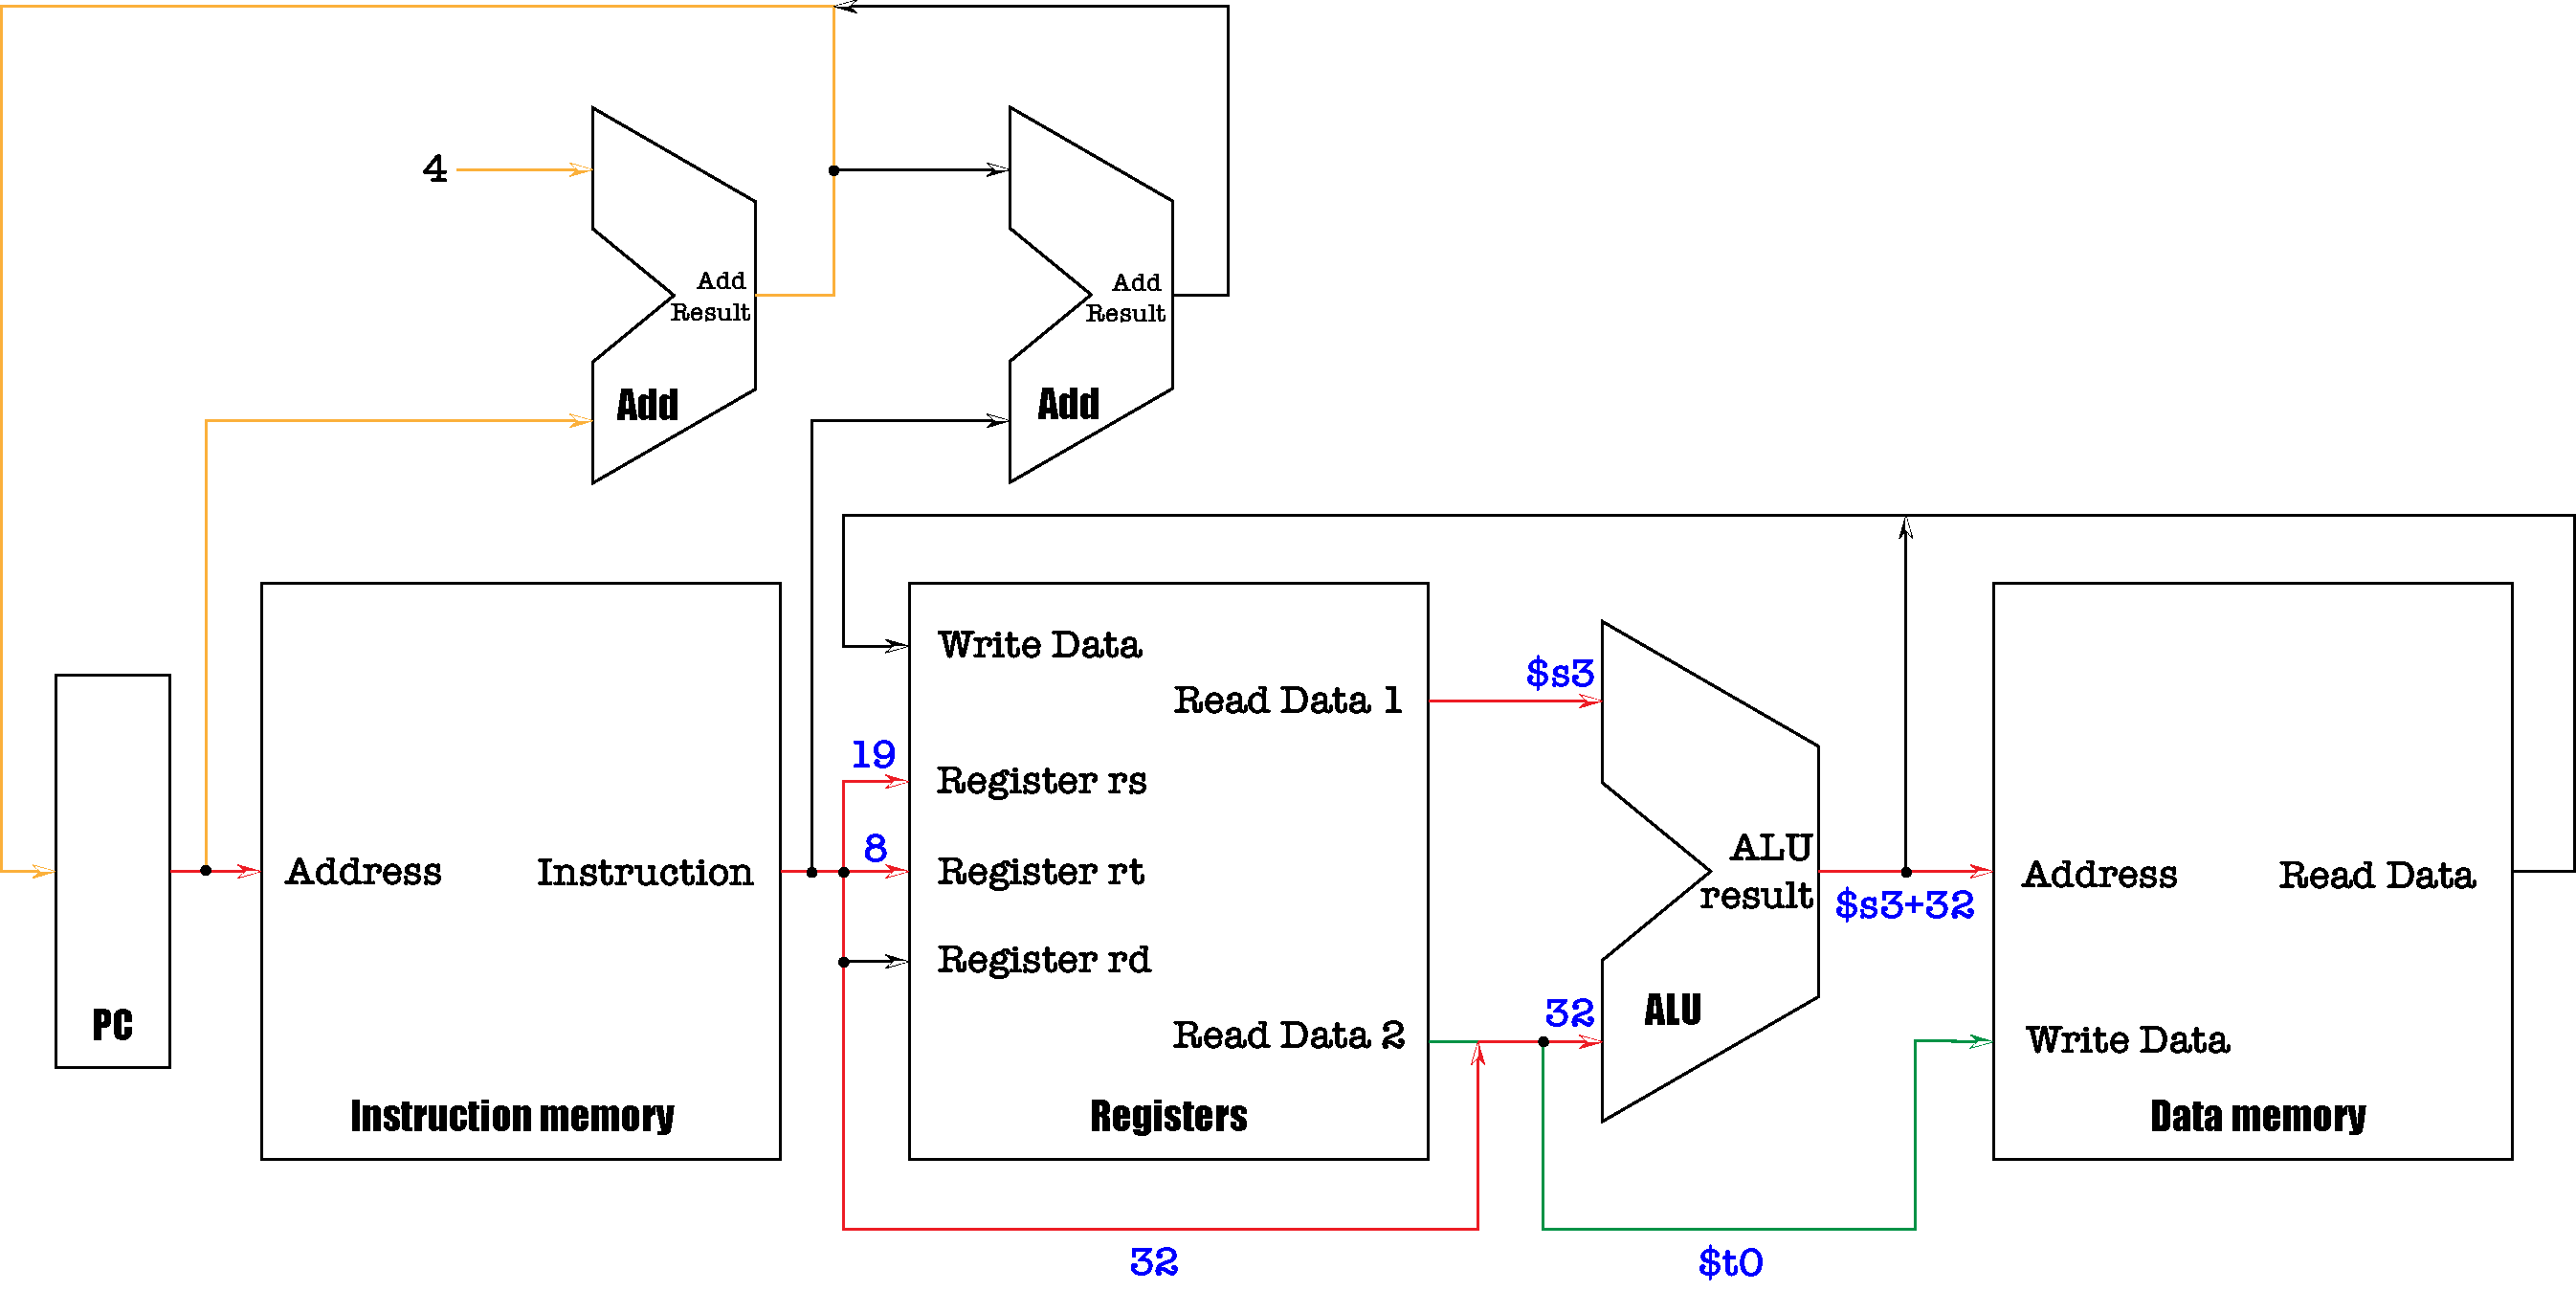
\includegraphics[scale=.3]{img/figure27.pdf}
\end{figure}
上图表示\verb|sw $t0, 32($s3)|指令执行的\textcolor{myred}{源数据流向}, \textcolor{mygreen}{结果流向}, \textcolor{myyellow}{\texttt{PC}改变}.
\item \texttt{add}操作 \par
我们以\verb|add $t0, $s1, $s2|为例, 首先, 将上述指令转化为十进制的样式:
\begin{table}[H]
\centering
\begin{tabularx}{\textwidth}{|Z|Z|Z|Z|Z|Z|}
\hline
\verb|0(op)| & \verb|17(rs)| & \verb|18(rt)| & \verb|8(rd)| & \verb|0(shamt)| & \verb|32(funct)| \\
\hline
\end{tabularx}
\end{table}
然后, 将数据流在电路图中表示:
\begin{figure}[H]
\centering
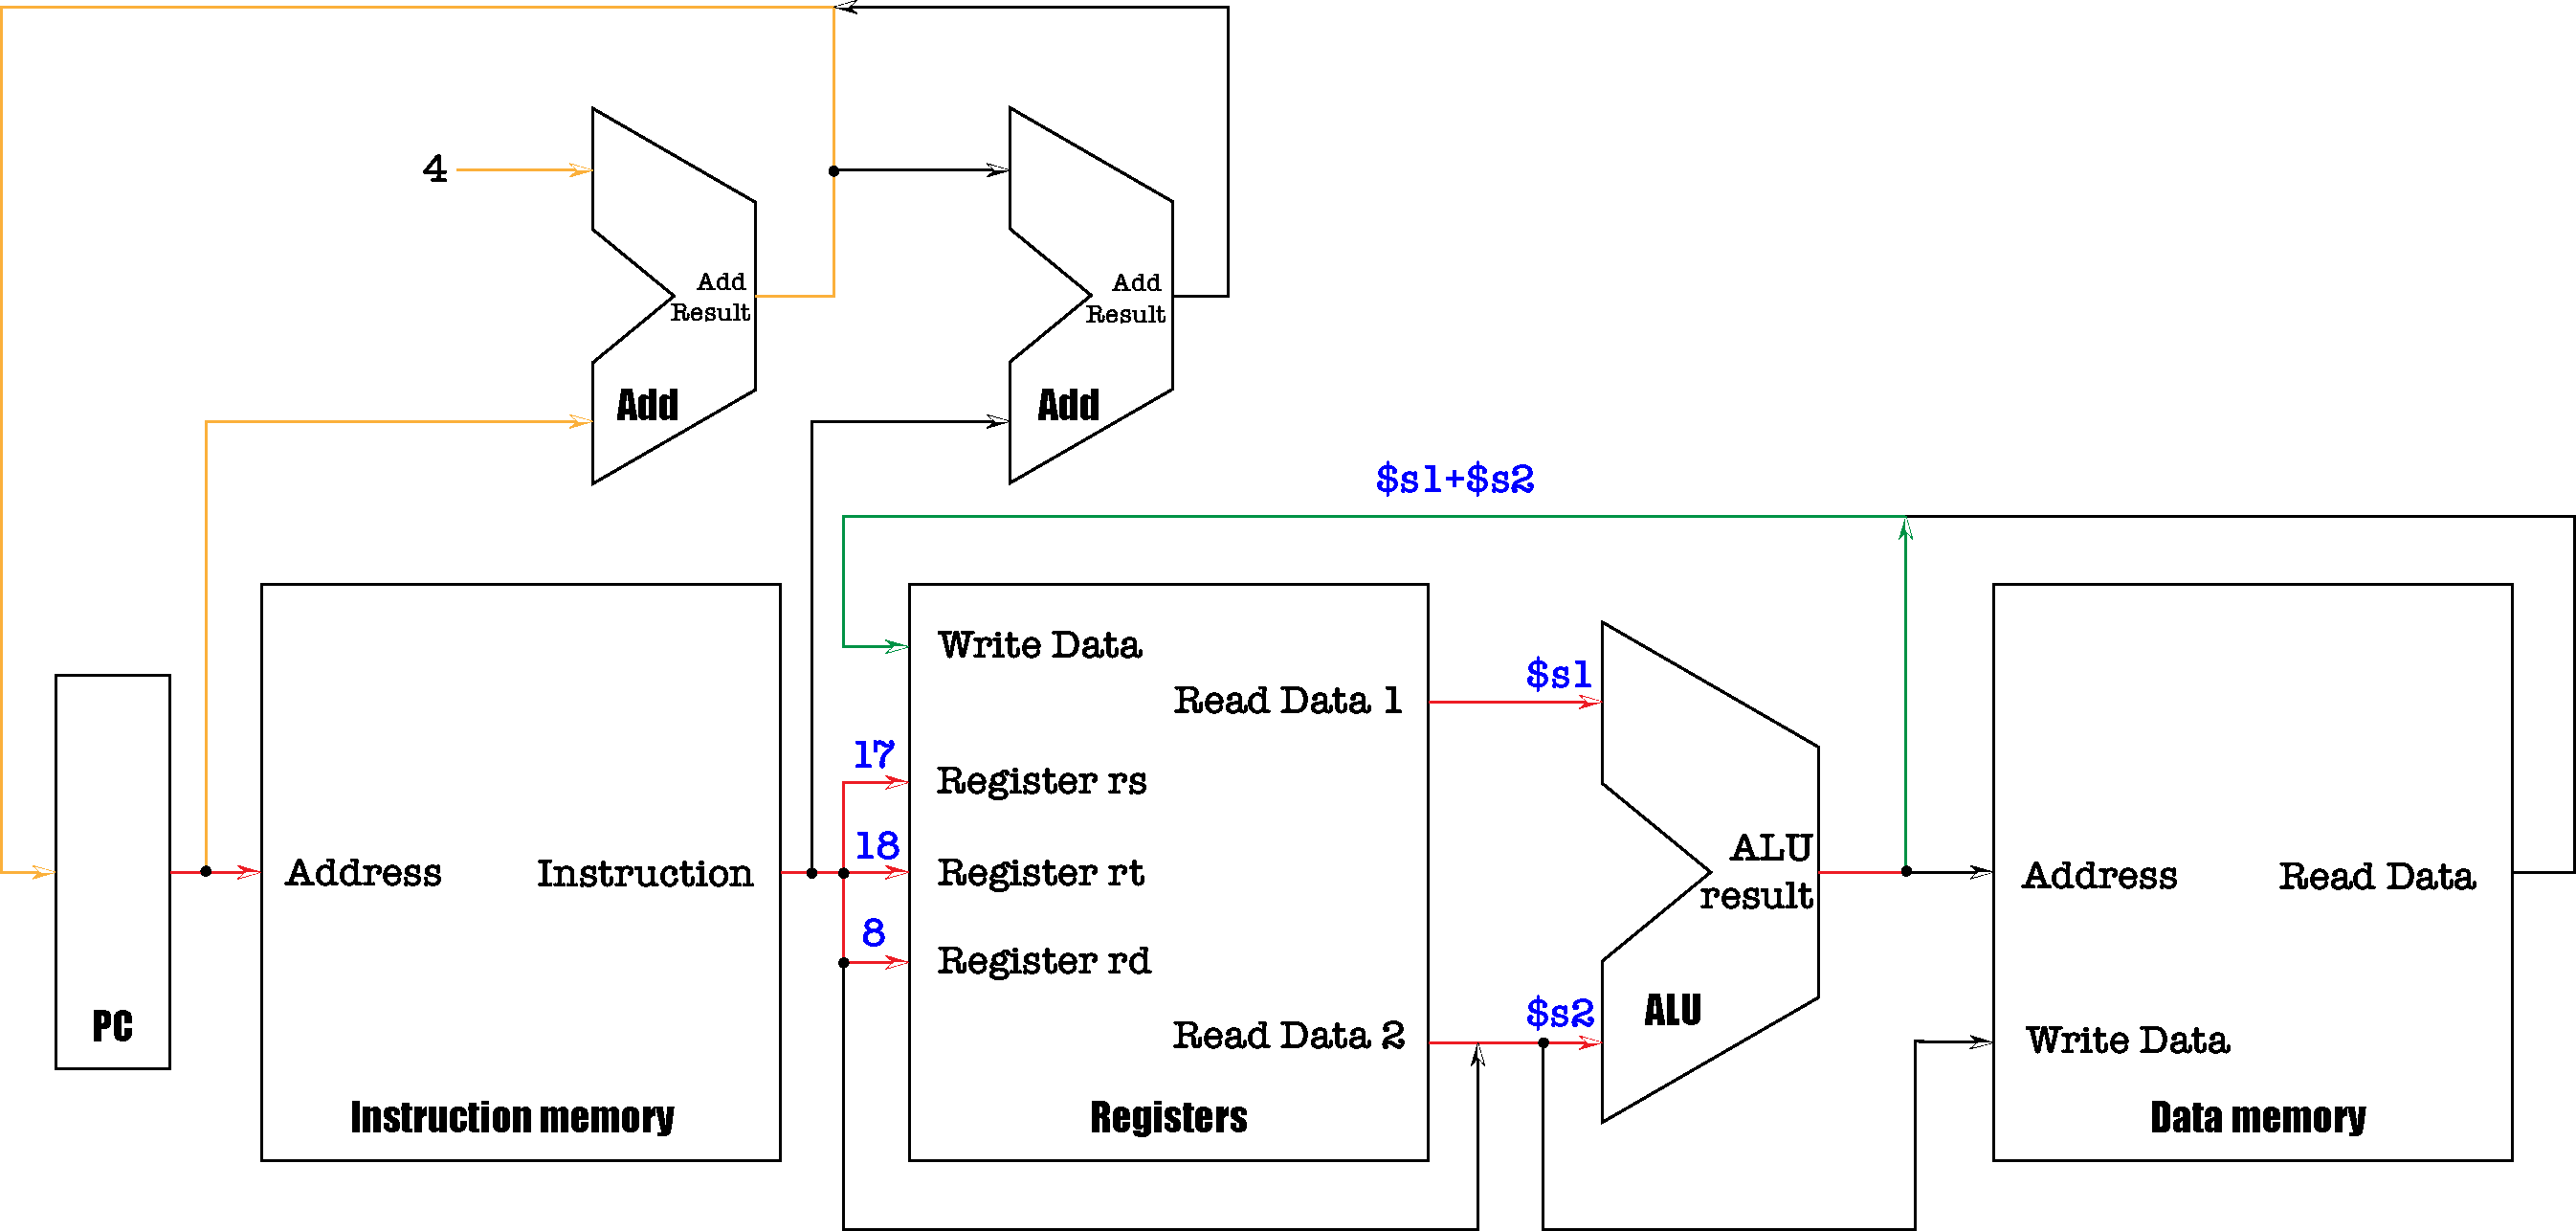
\includegraphics[scale=.3]{img/figure28.pdf}
\end{figure}
上图表示\verb|add $t0, $s1, $s2|指令执行的\textcolor{myred}{源数据流向}, \textcolor{mygreen}{结果流向}, \textcolor{myyellow}{\texttt{PC}改变}.
\item \texttt{beq}操作 \par
我们以\verb|beq $s3, $t0, label|为例, 首先, 将上述指令转化为十进制的样式:
\begin{table}[H]
\centering
\begin{tabularx}{\textwidth}{|Z|Z|Z|Z|}
\hline
\verb|4(op)| & \verb|19(rs)| & \verb|8(rt)| & \verb|label(offset)| \\
\hline
\end{tabularx}
\end{table}
然后, 将数据流在电路图中表示:
\begin{figure}[H]
\centering
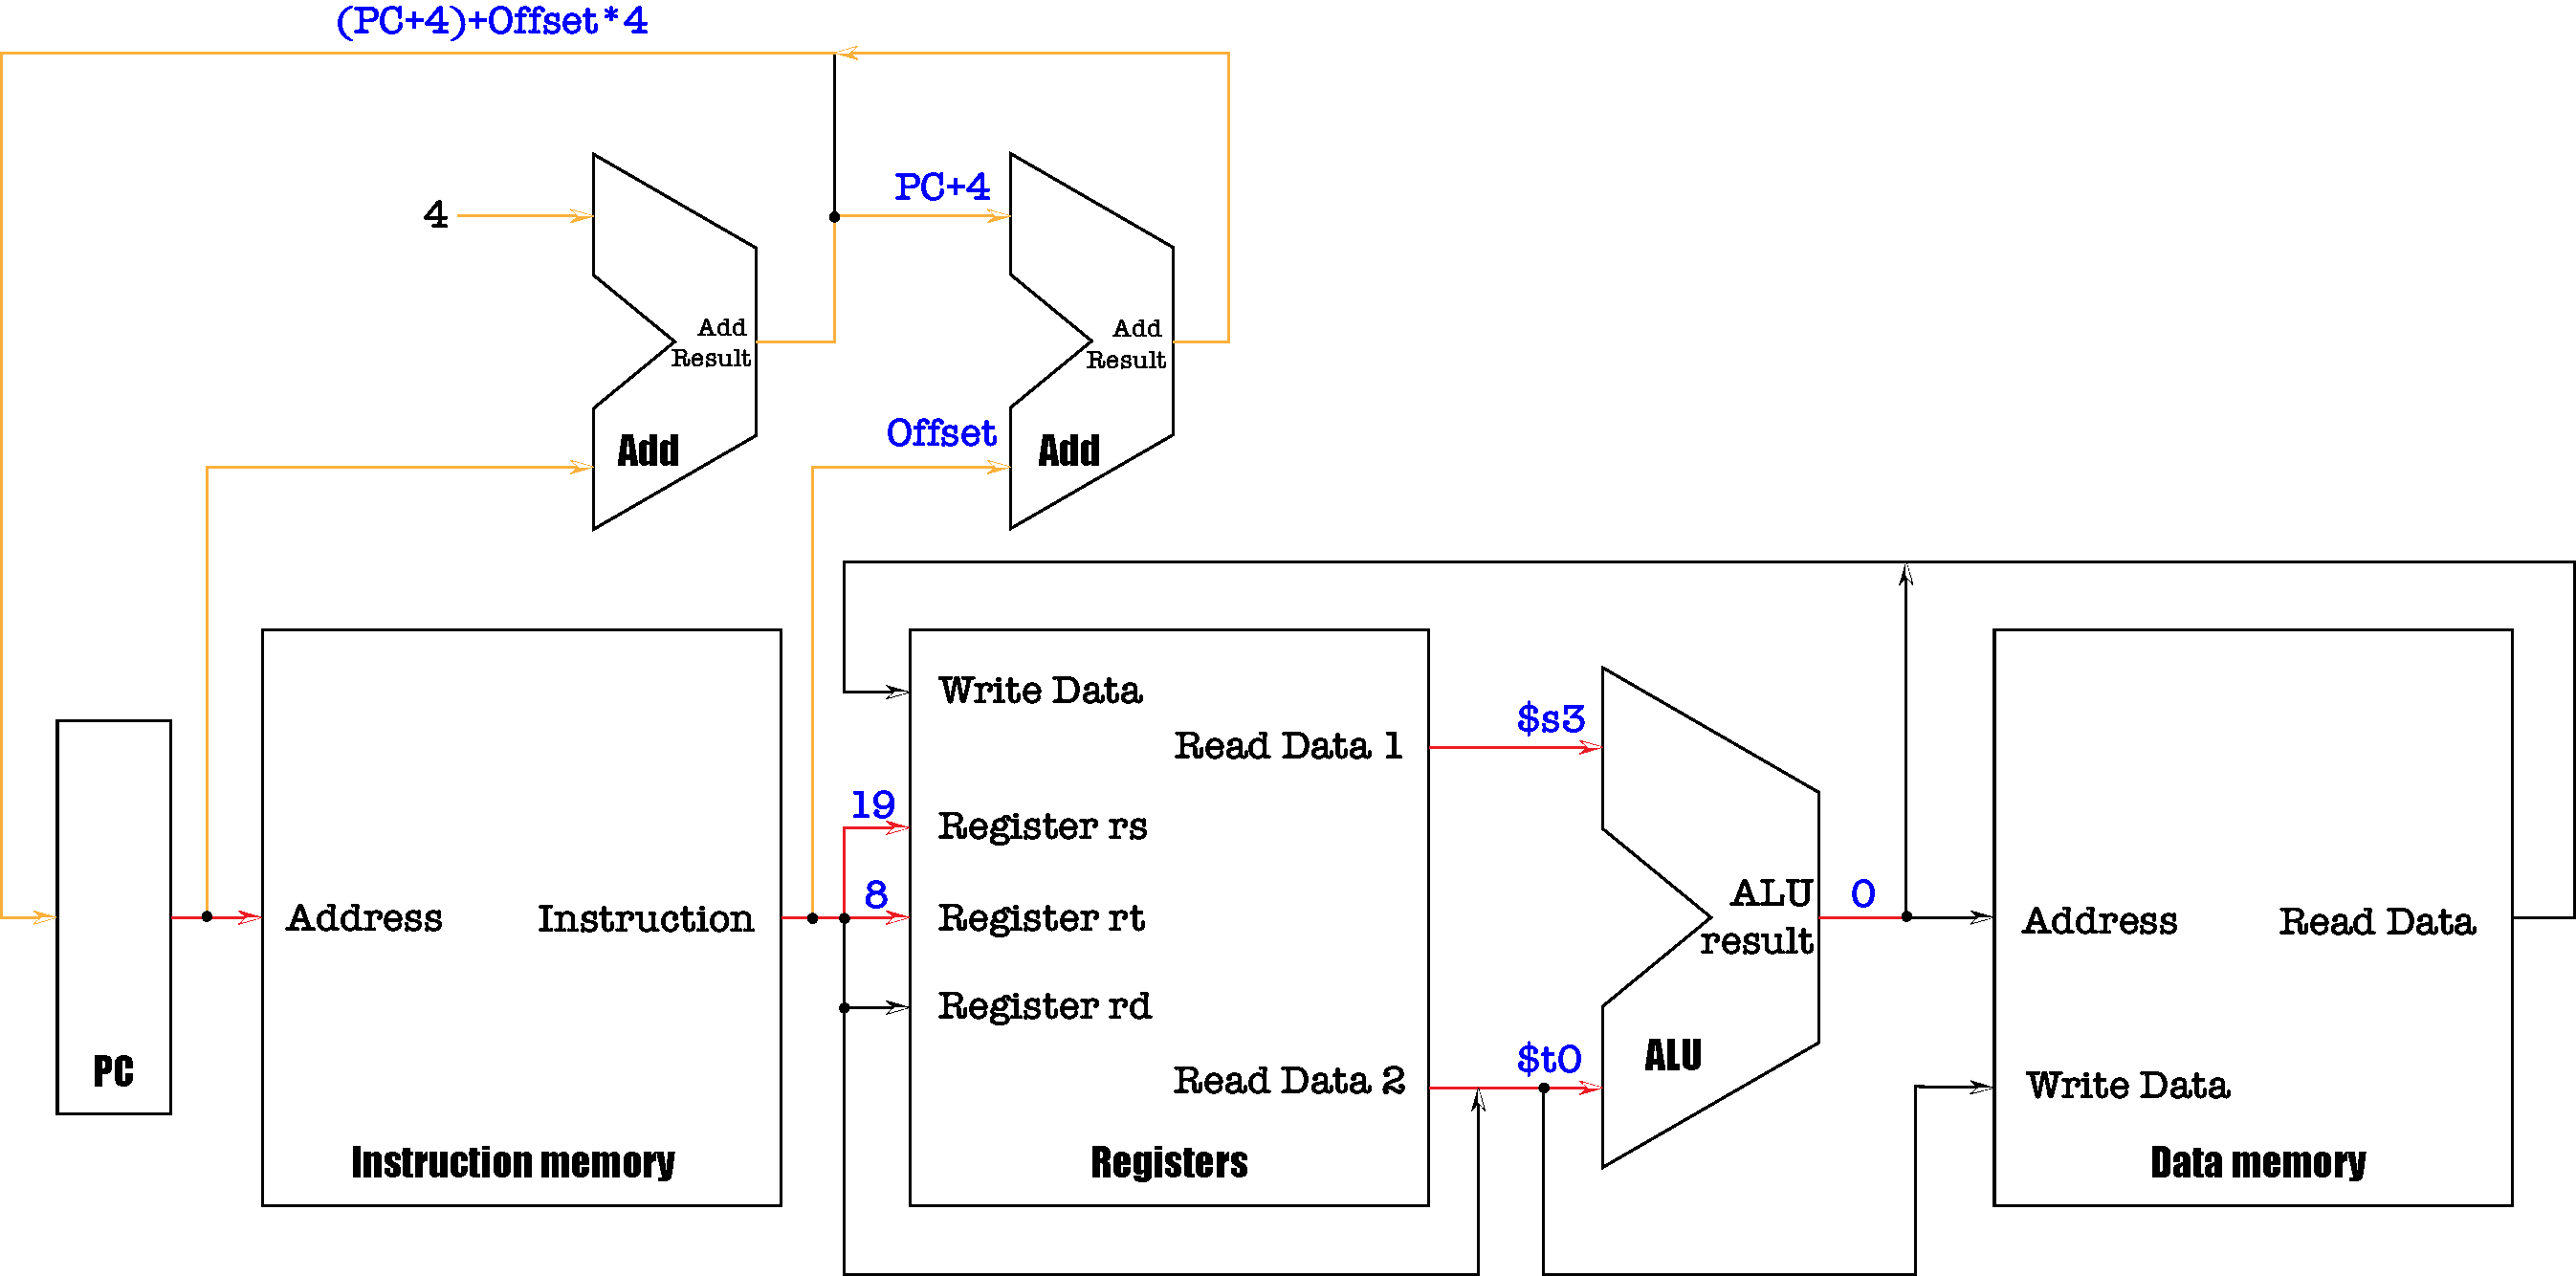
\includegraphics[scale=.3]{img/figure29.pdf}
\end{figure}
上图表示\verb|beq $s3, $t0, label|指令执行的\textcolor{myred}{源数据流向}, \textcolor{myyellow}{\texttt{PC}改变}.
\item \texttt{j}操作 \par
我们以\verb|j Addr|为例, 在电路图中表示为:
\begin{figure}[H]
\centering
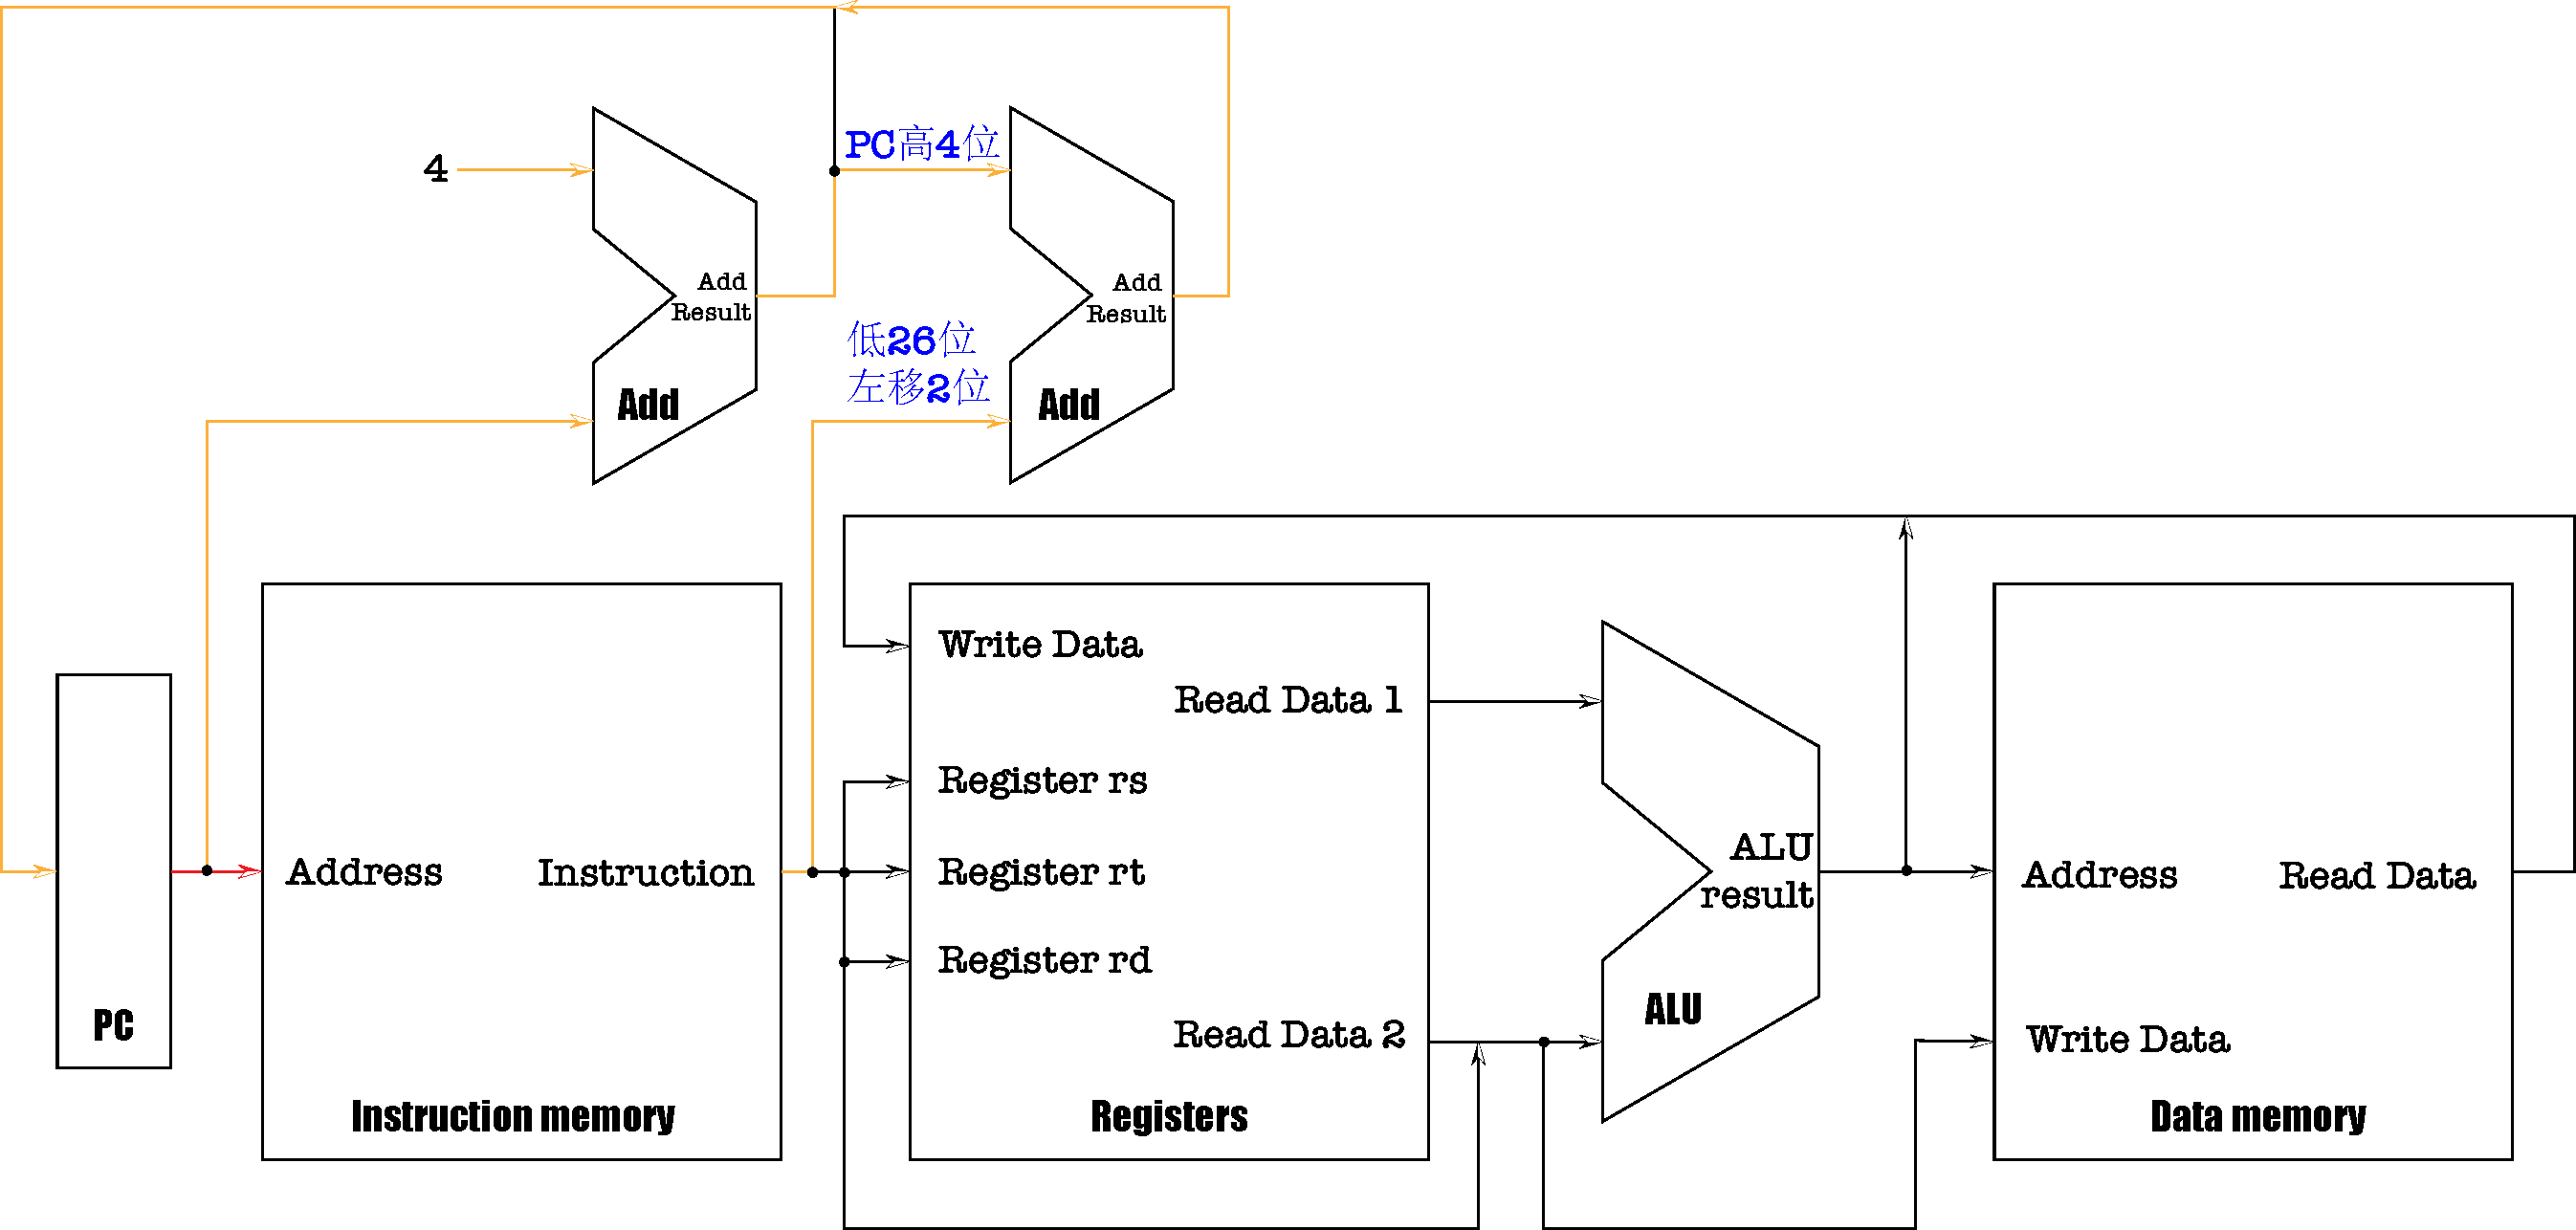
\includegraphics[scale=.3]{img/figure30.pdf}
\end{figure}
上图表示\verb|j Addr|指令执行的\textcolor{myyellow}{\texttt{PC}改变}.
\end{enumerate}
\subsubsection{增加选择器和控制器}
观察上面的电路图我们会发现, 有很多分支电路
\begin{figure}[H]
\centering
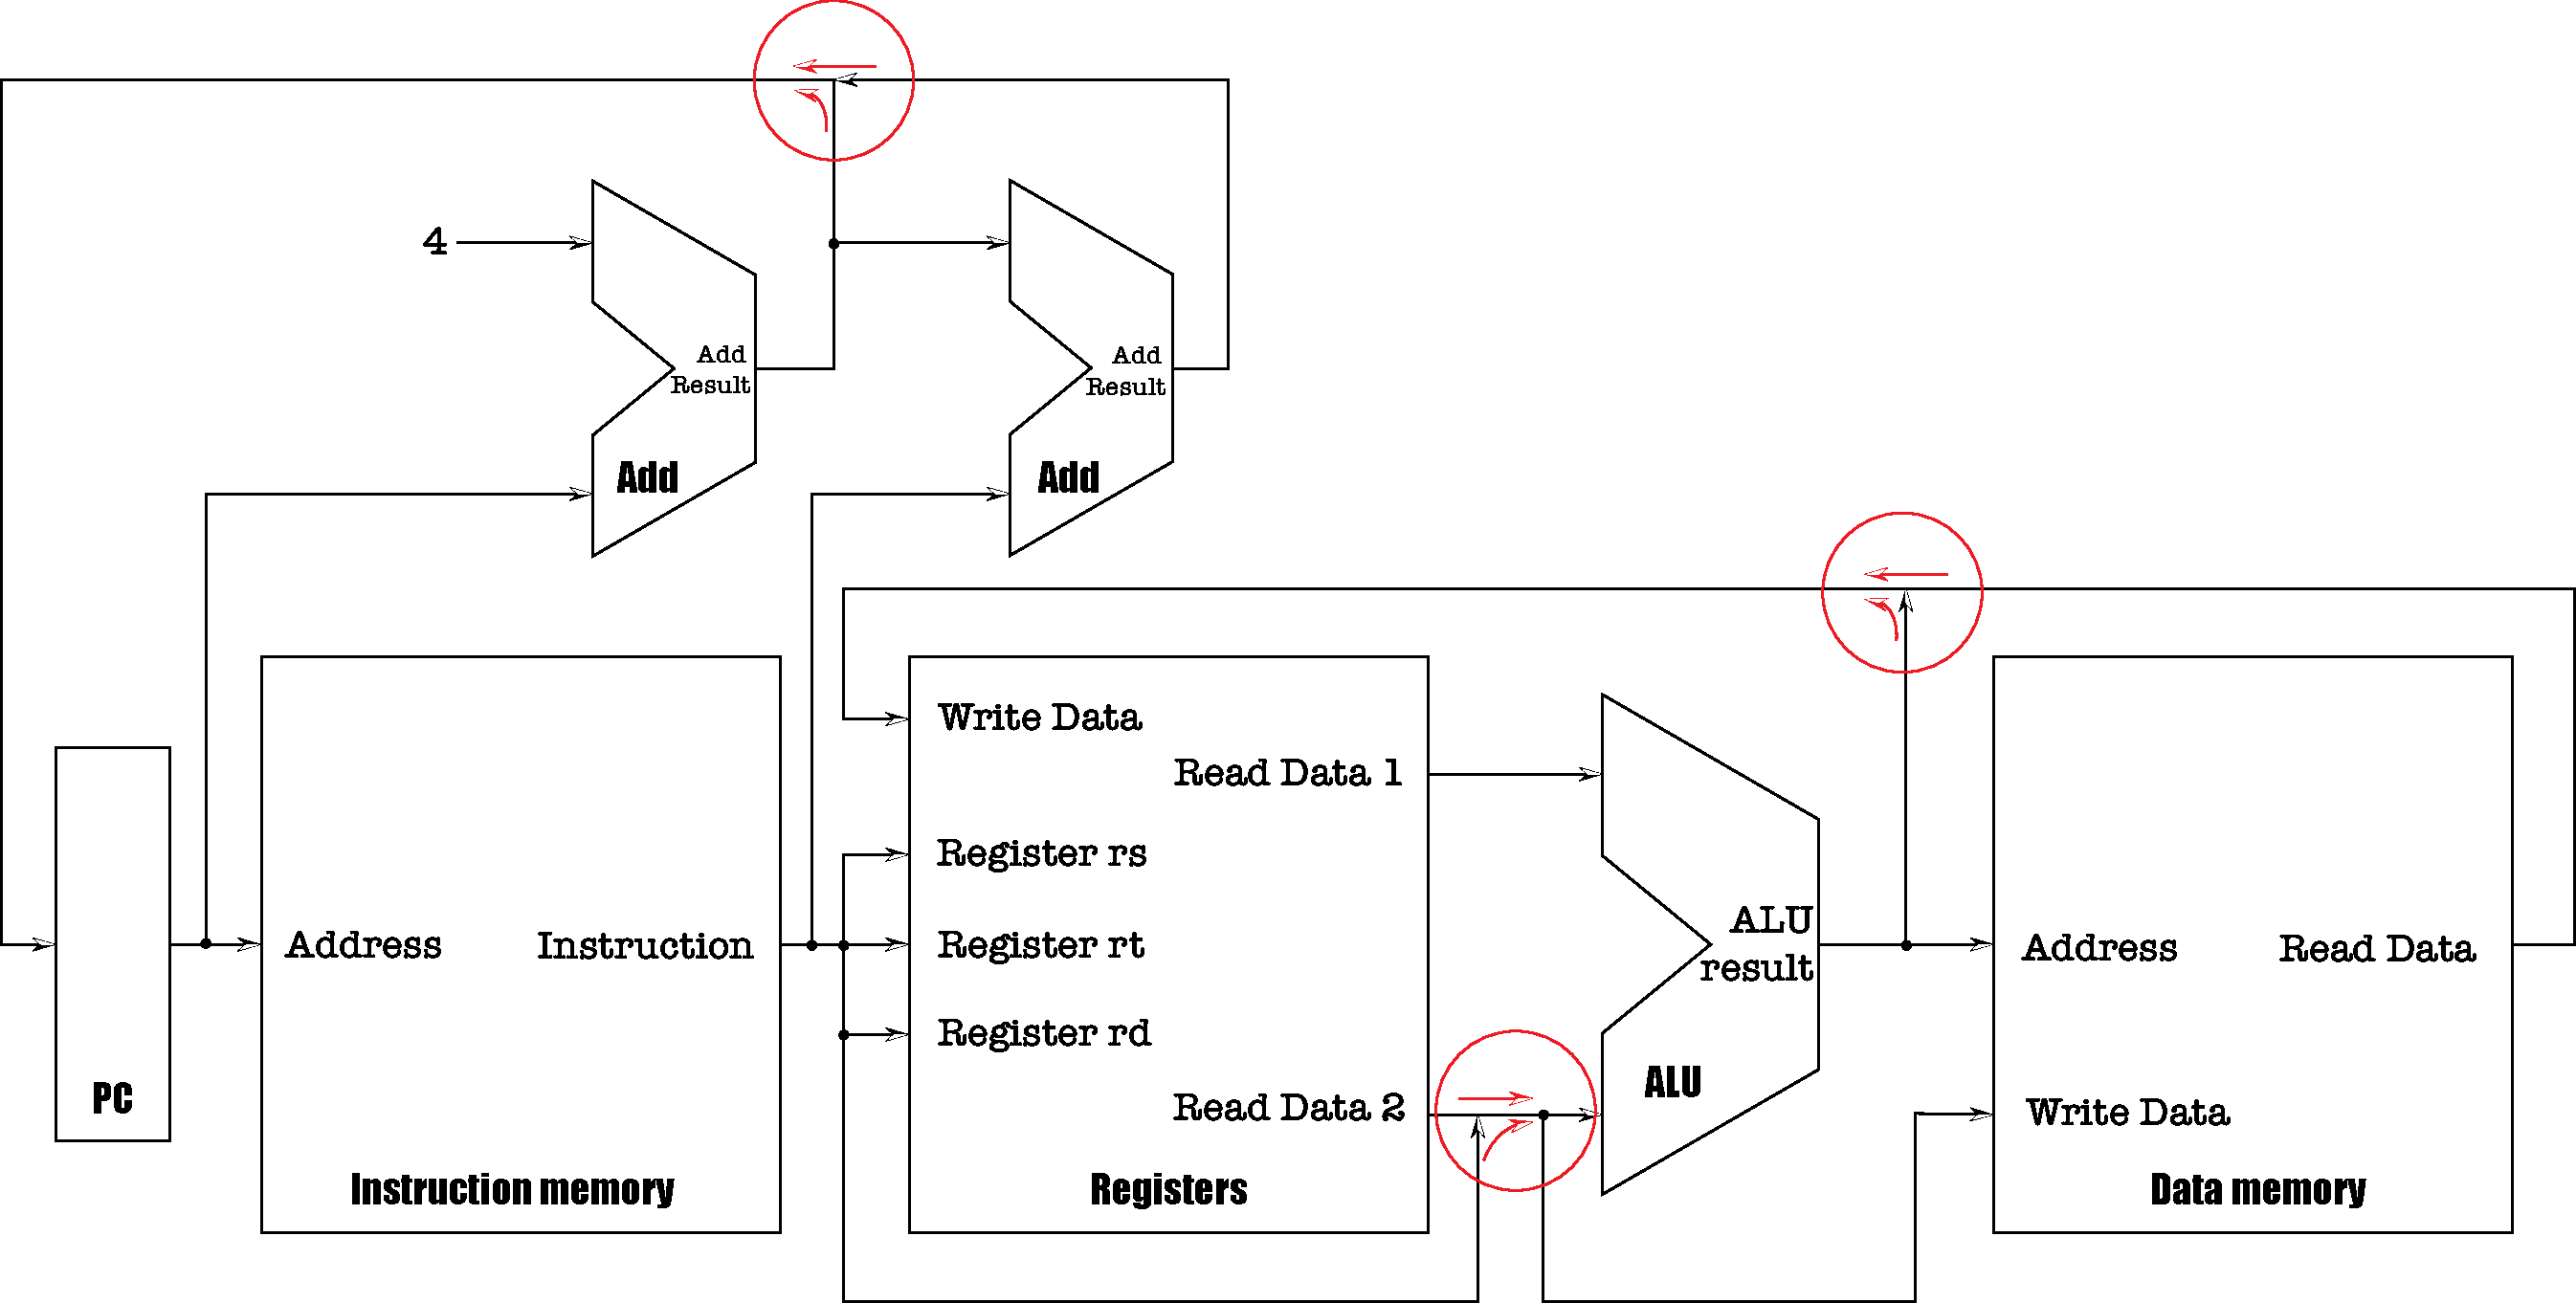
\includegraphics[scale=.3]{img/figure31.pdf}
\end{figure}
所以数据到底应该走哪一条呢? 我们需要添加选择器和控制器以选择数据:
\begin{itemize}
\item \verb|1|号选择器+控制器
\begin{figure}[H]
\centering
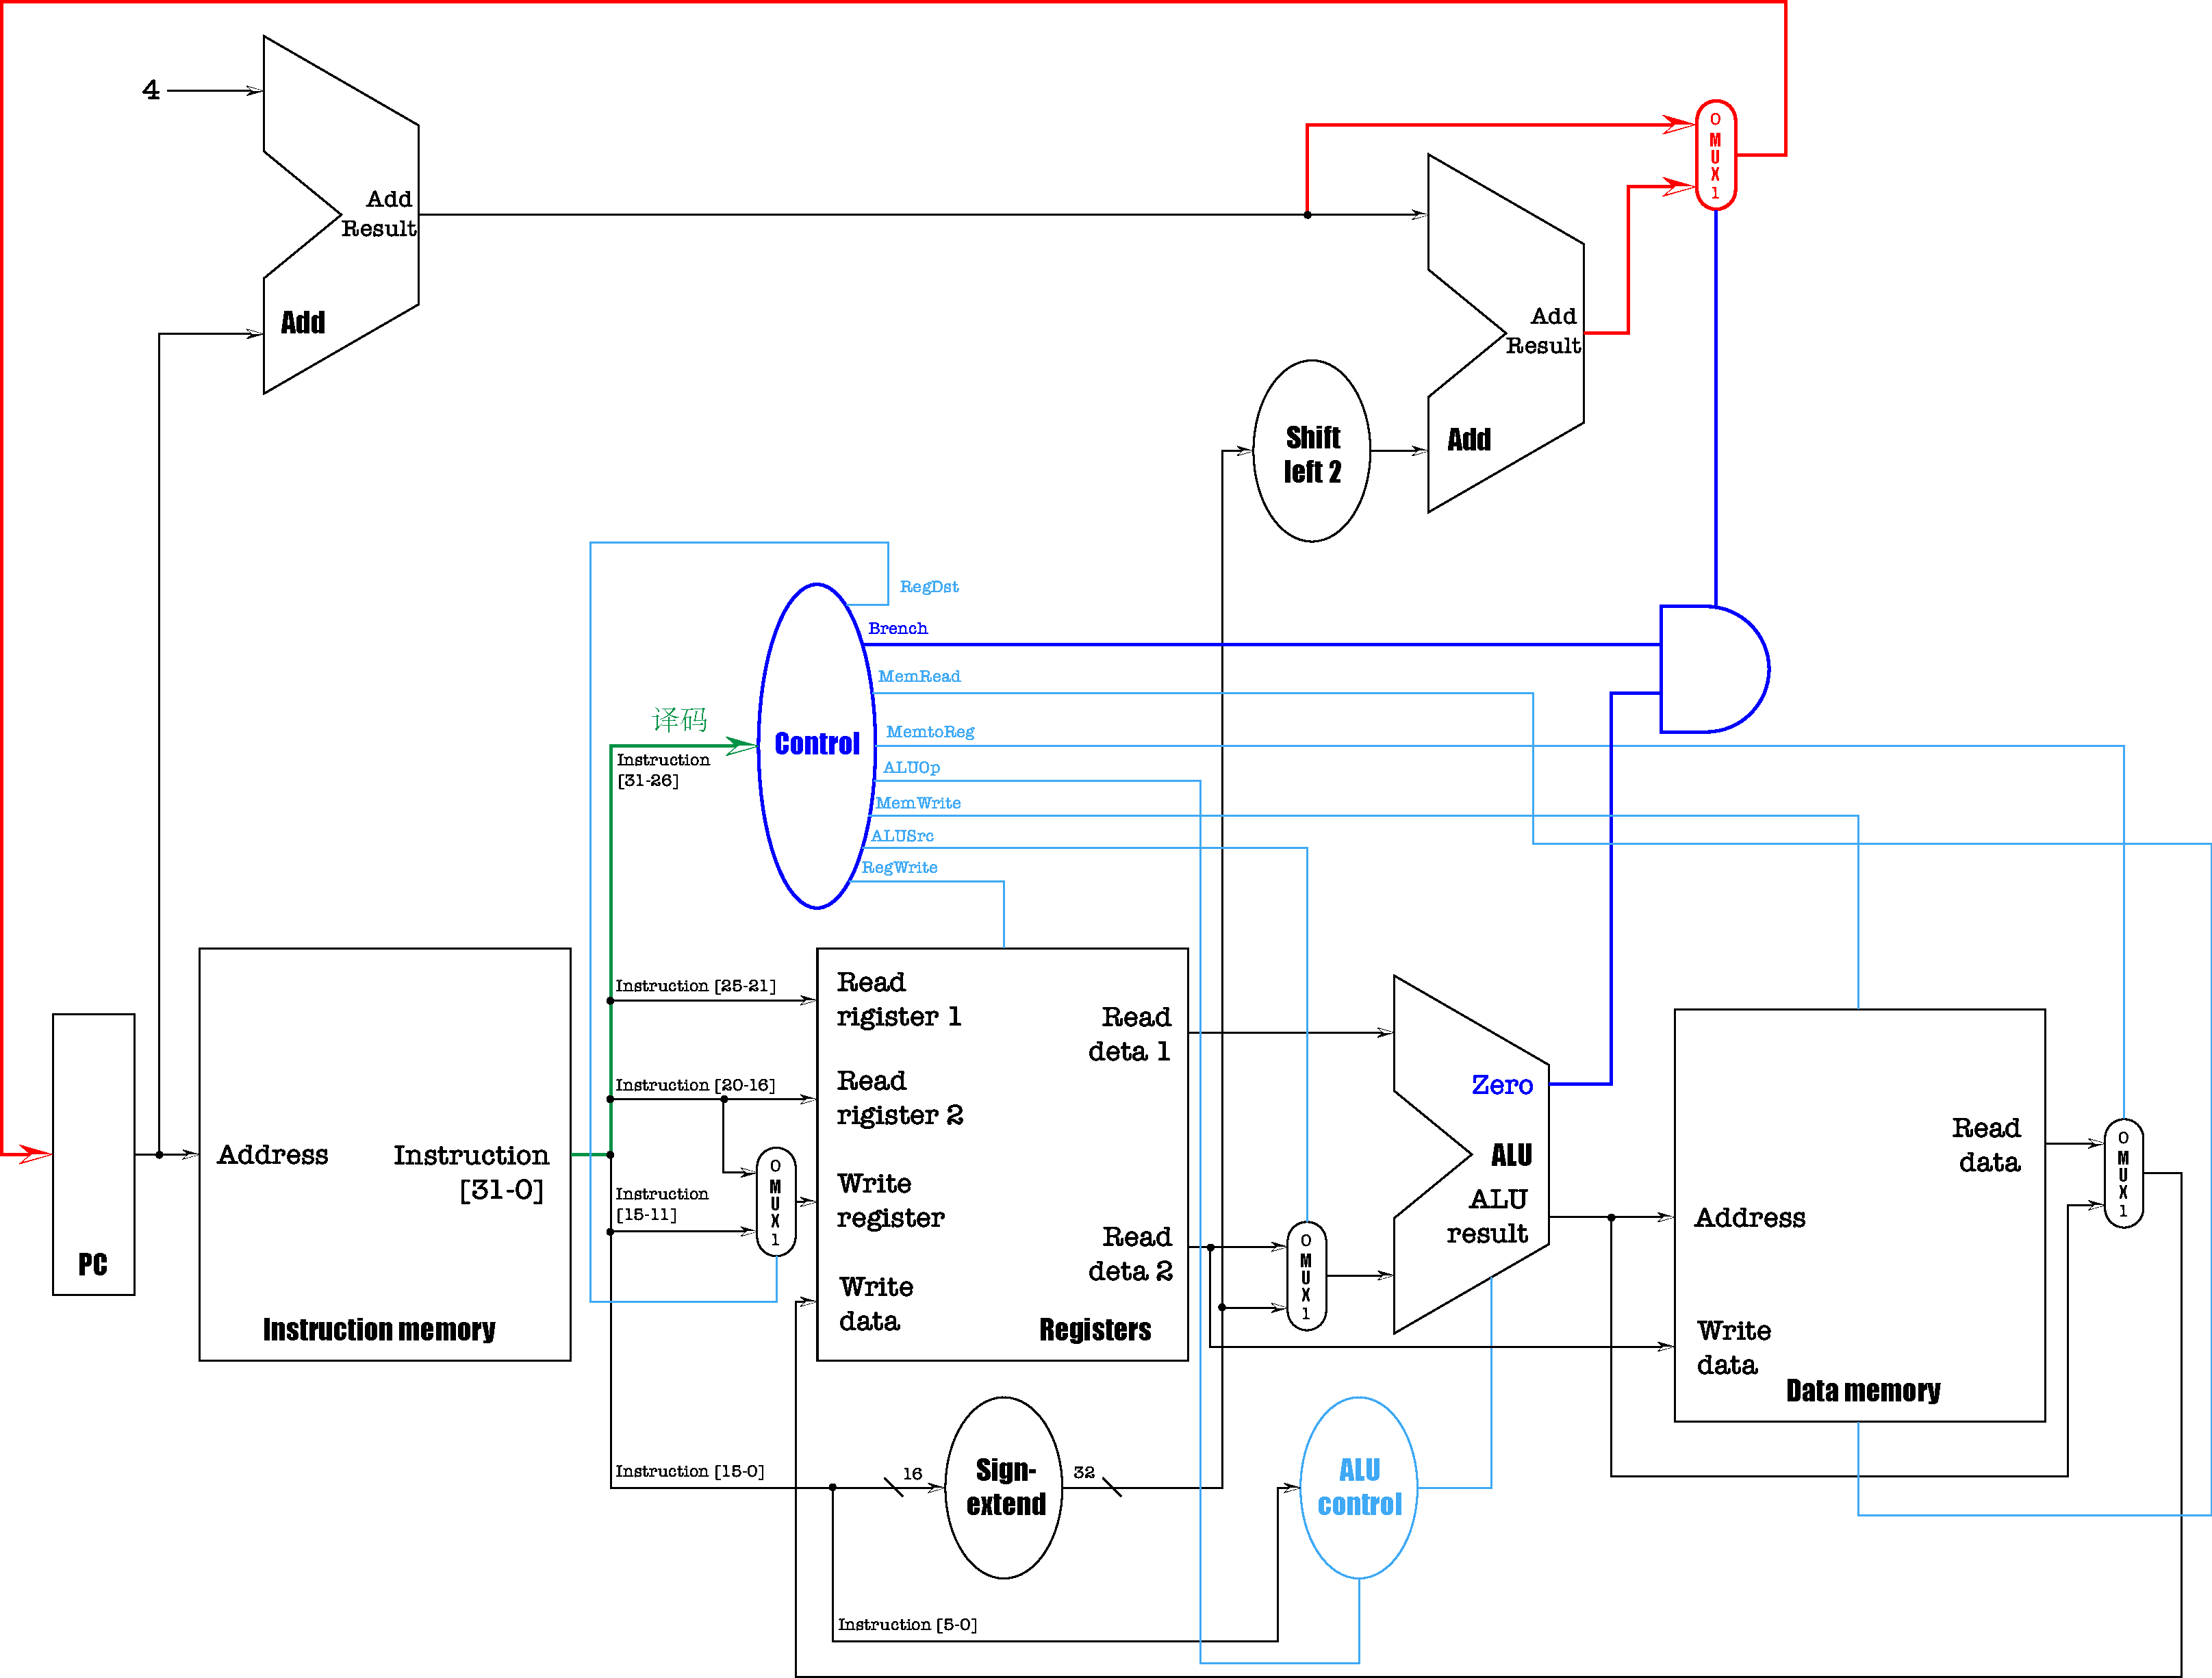
\includegraphics[scale=.2]{img/figure32.pdf}
\end{figure}
该选择器的作用是选择\verb|PC+4|还是\verb|PC+4+Offset*4|, 条件由控制器控制, 若指令译码结果\verb|op|为\verb|beq|指令, 则\verb|ALU|如果相减为\verb|0|则否, 选择器选择\verb|PC=PC+4+Offset*4|.
\item \verb|2|号选择器+控制器
\begin{figure}[H]
\centering
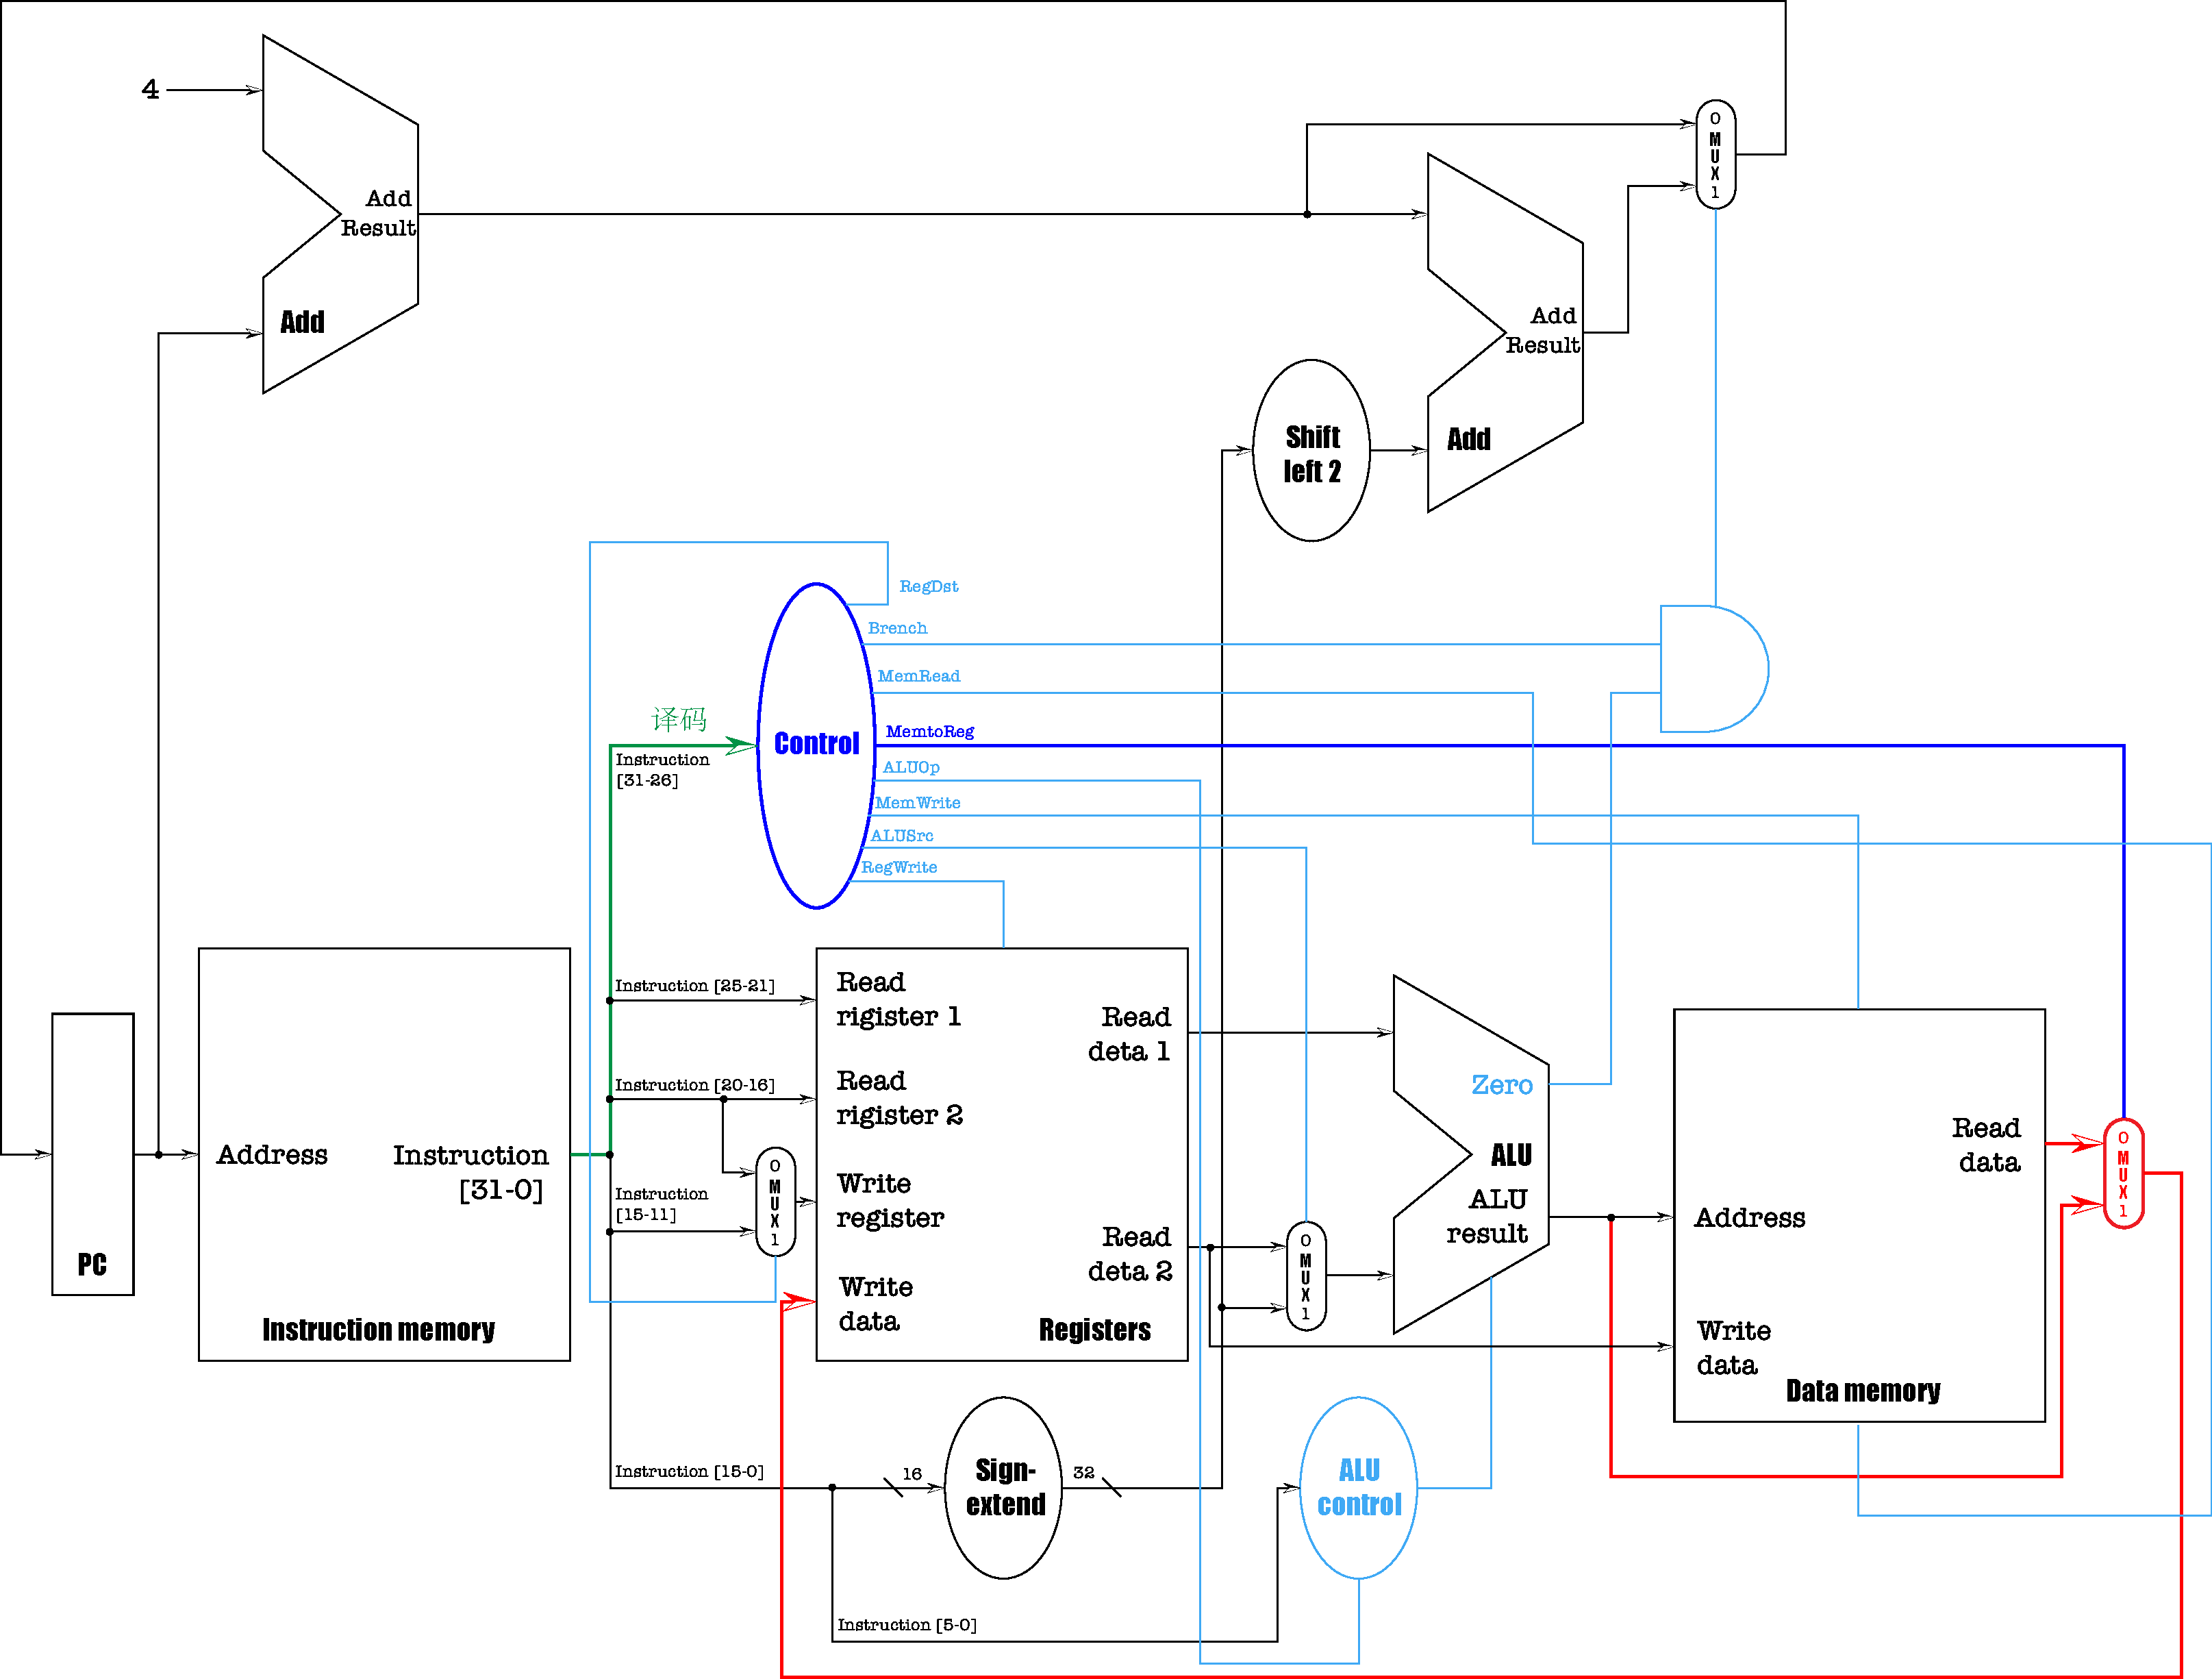
\includegraphics[scale=.2]{img/figure33.pdf}
\end{figure}
该选择器的作用是选择\verb|lw|还是逻辑运算指令\verb|add,sub...|, 前者存入寄存器的是从主存中读出的数据, 而后者是\verb|ALU|计算的数据或者是寄存器置\verb|0|/\verb|1|.
\item \verb|3|号选择器+控制器
\begin{figure}[H]
\centering
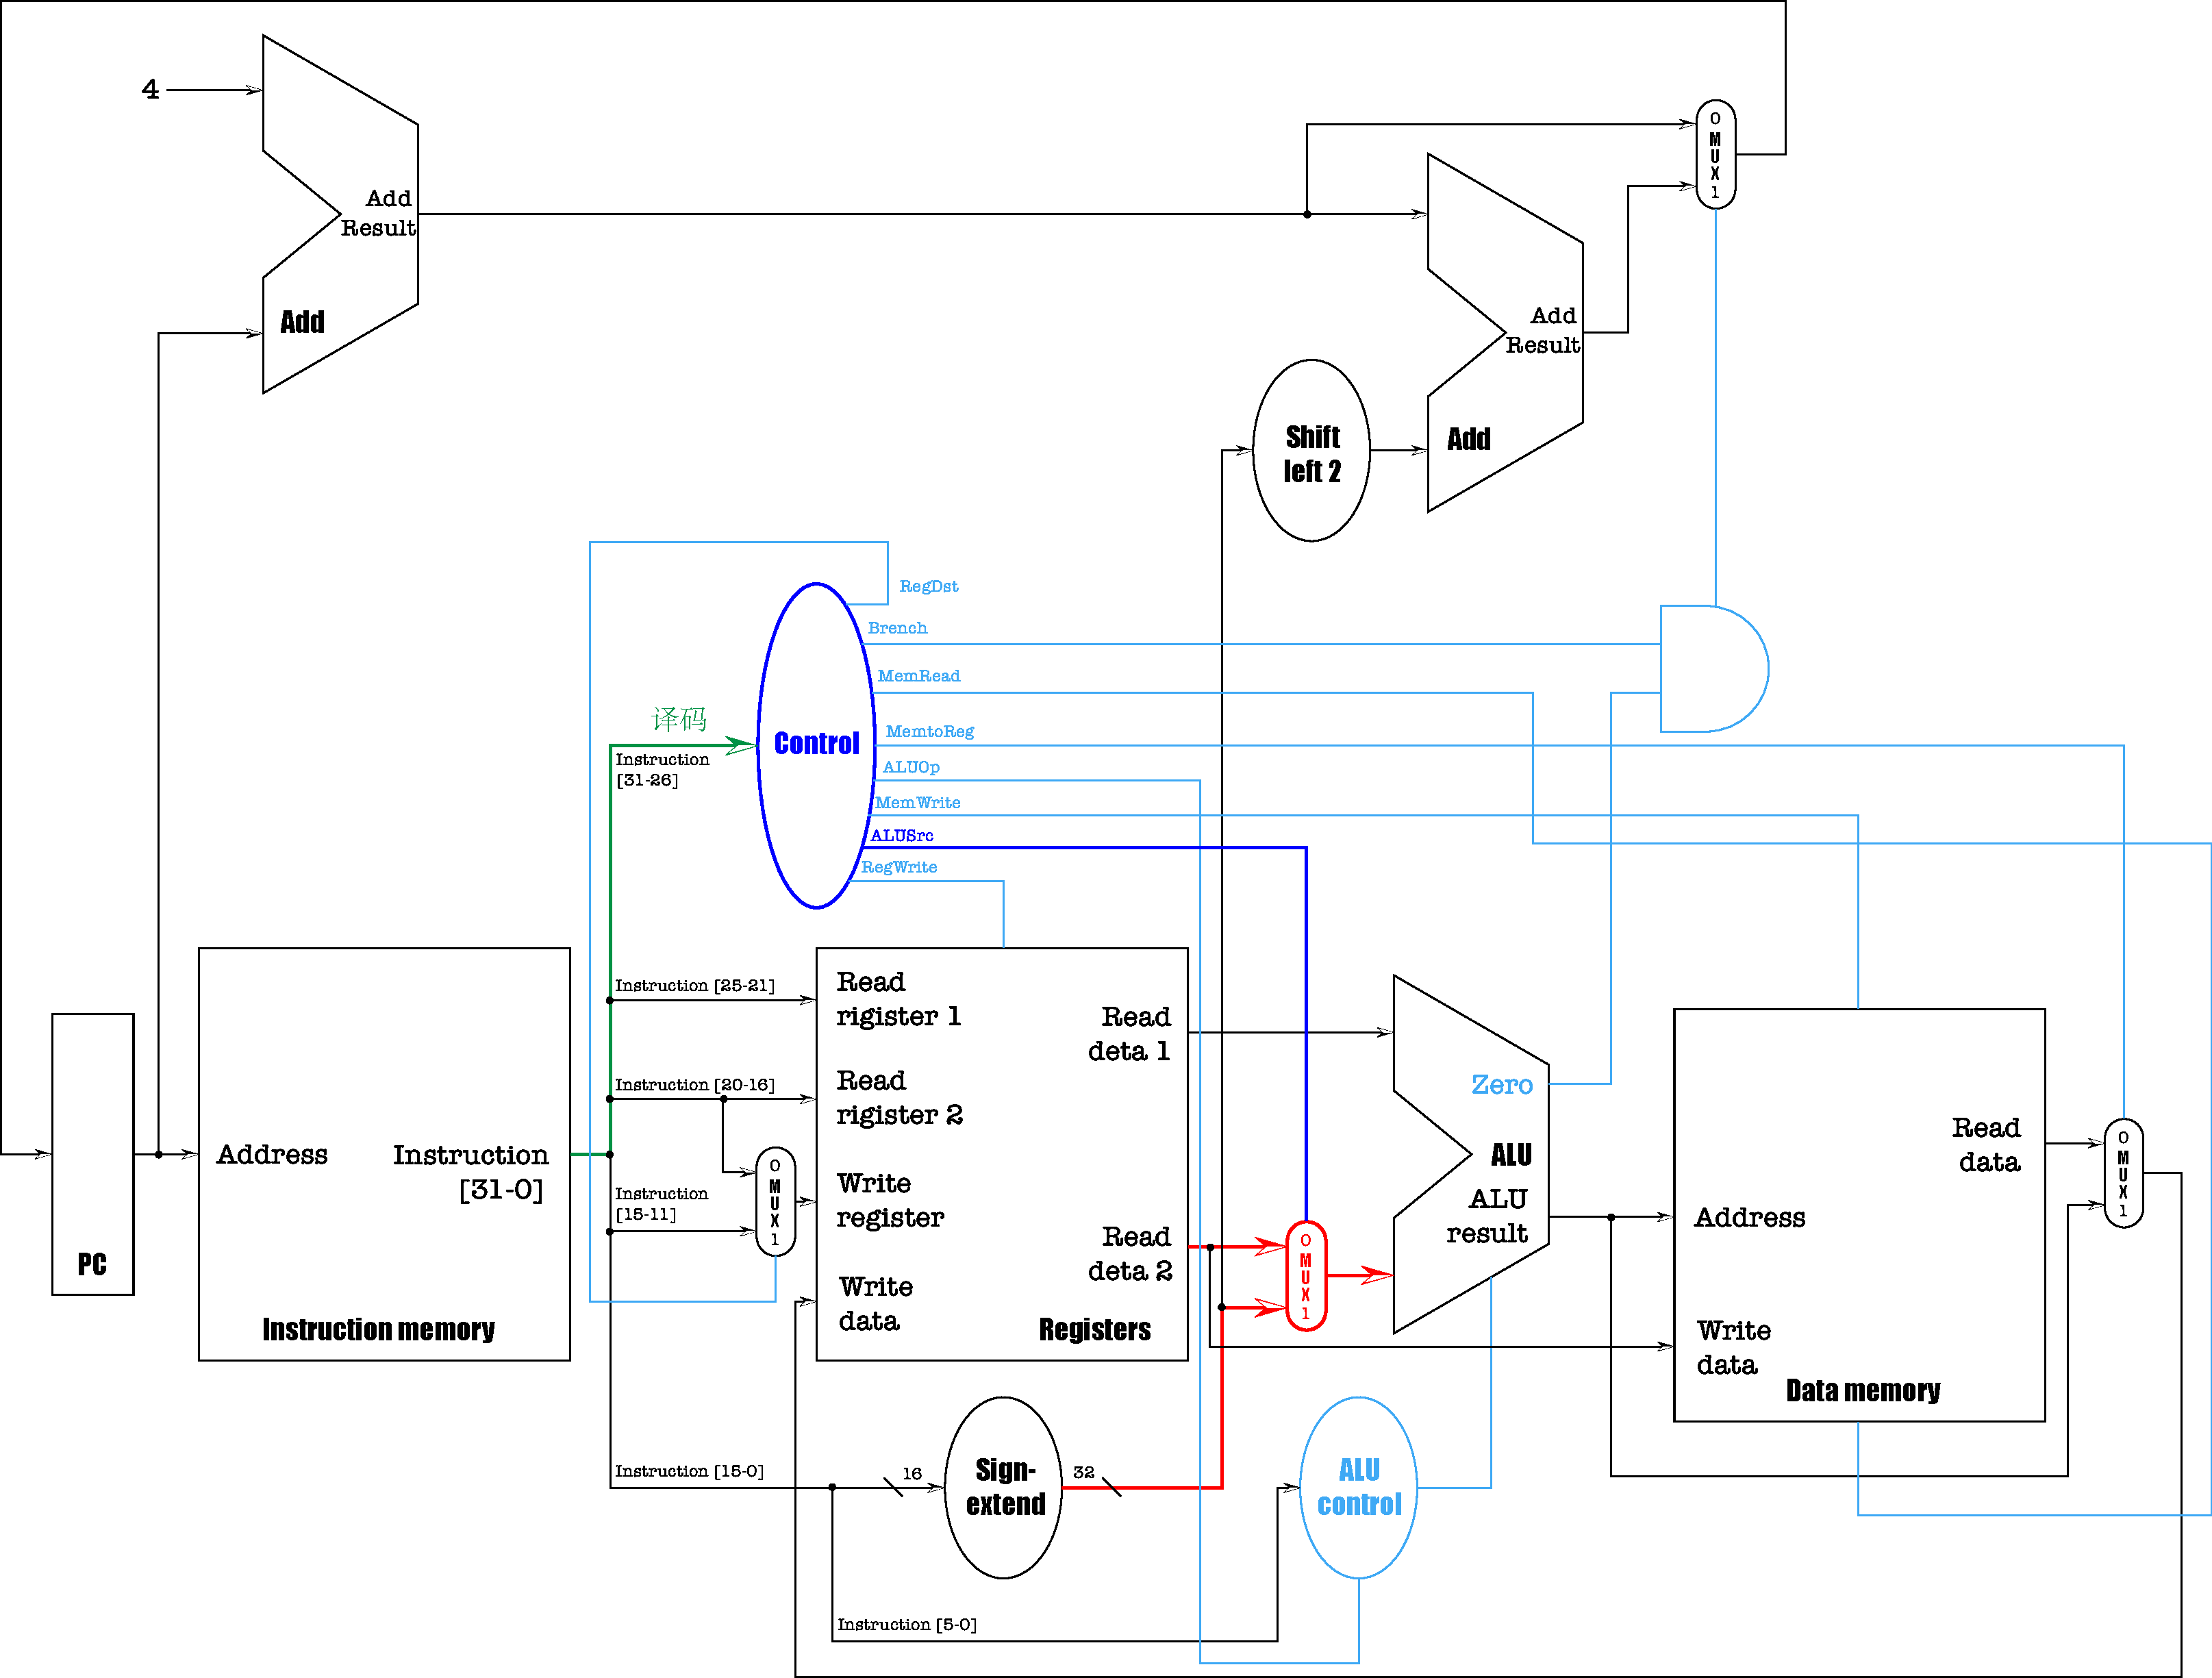
\includegraphics[scale=.2]{img/figure34.pdf}
\end{figure}
该选择器的作用是选择\verb|lw, sw|指令的\verb|Offset|, 还是算数逻辑命令指明的寄存器的值.
\item 其余控制器
\begin{figure}[H]
\centering
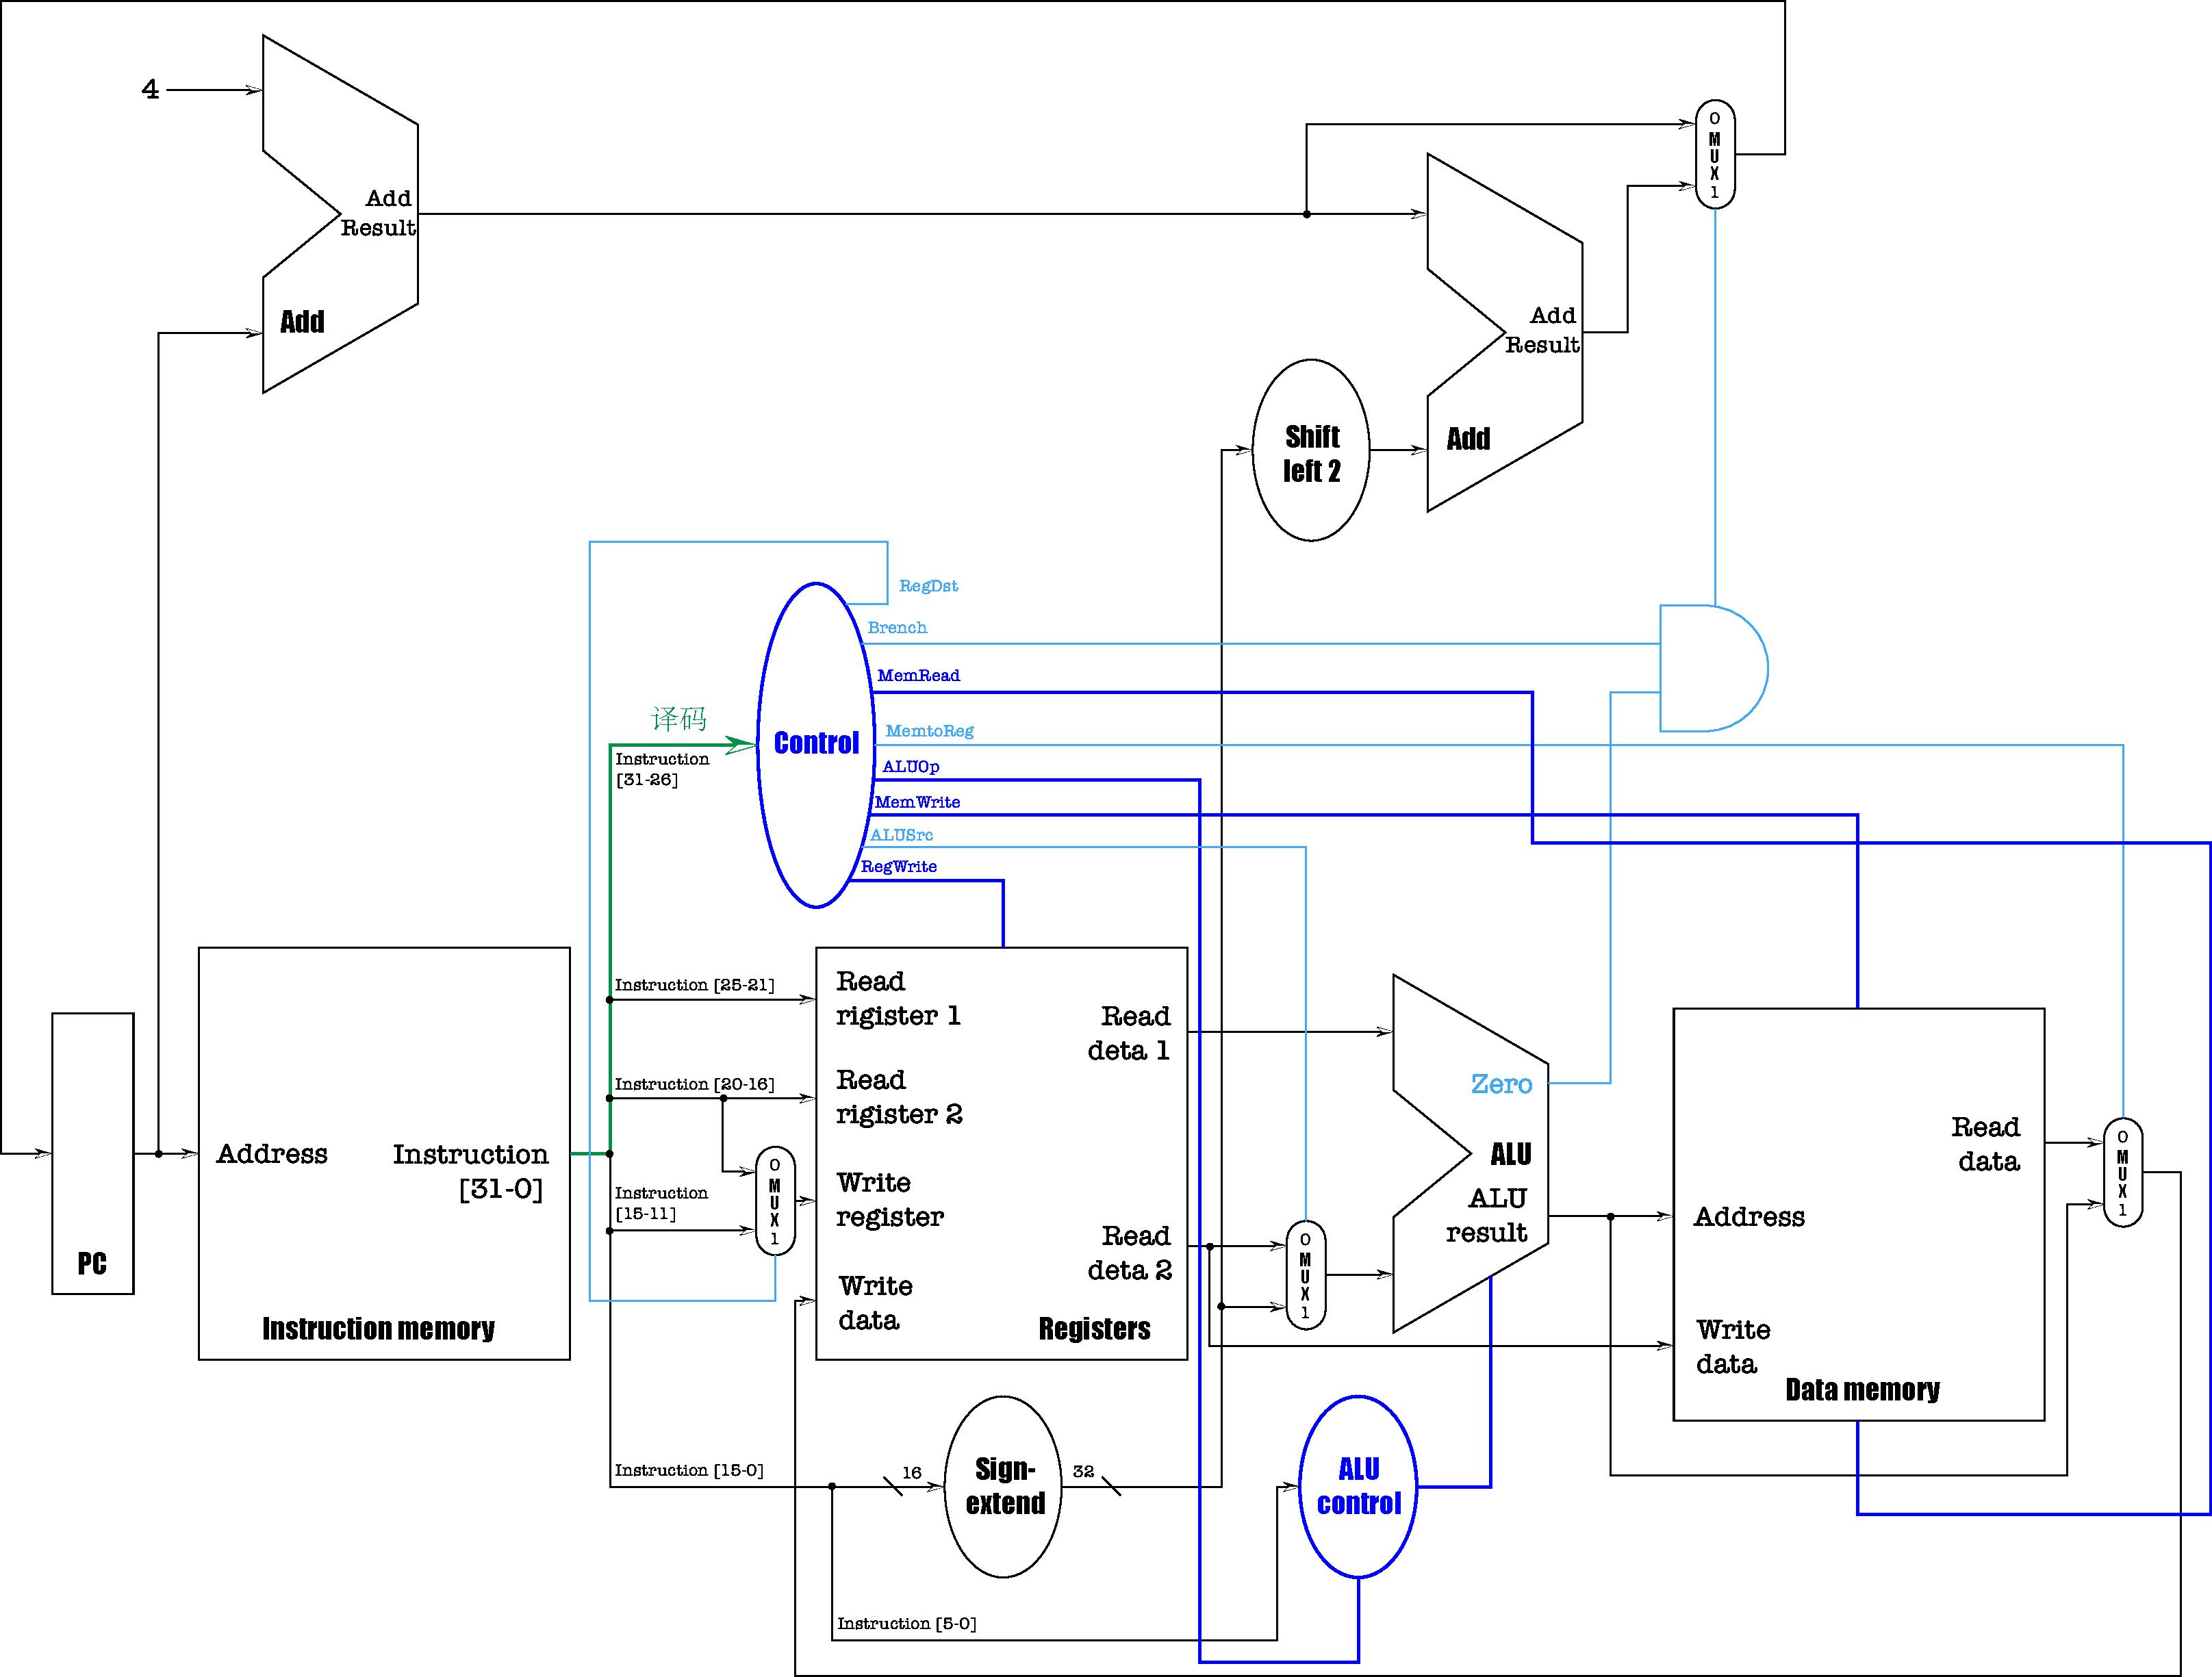
\includegraphics[scale=.2]{img/figure35.pdf}
\end{figure}
用于控制寄存器, 存储器的读写, \verb|ALU|进行何种运算.
\end{itemize}
\section{流水线}
流水线是一种实现多条指令重叠执行的计数, 它改善的是系统的吞吐率, 每一个任务本身的执行时间不变. \par
\subsection{处理步骤}
\begin{figure}[H]
\centering
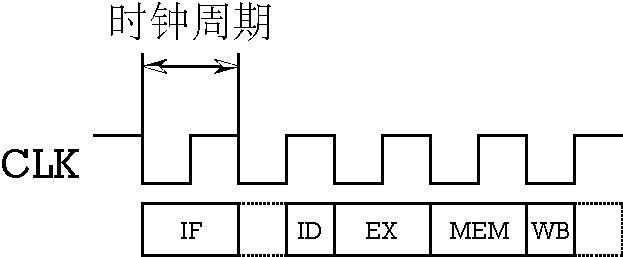
\includegraphics[scale=.5]{img/figure37.pdf}
\end{figure}
执行一条\verb|MIPS|指令包含\verb|5|个步骤:
\begin{enumerate}
\item \verb|Instructioin Fetch|: 从指令存储器中读出指令
\item \verb|Instruction Decode|: 指令译码, 并且同时读出寄存器的内容
\item \verb|Execute|: 执行操作或者计算地址
\item \verb|Memory Access|: 从数据存储器中读取操作数
\item \verb|Write Back|: 将结果写回寄存器
\end{enumerate}
从电路图上看:
\begin{figure}[H]
\centering
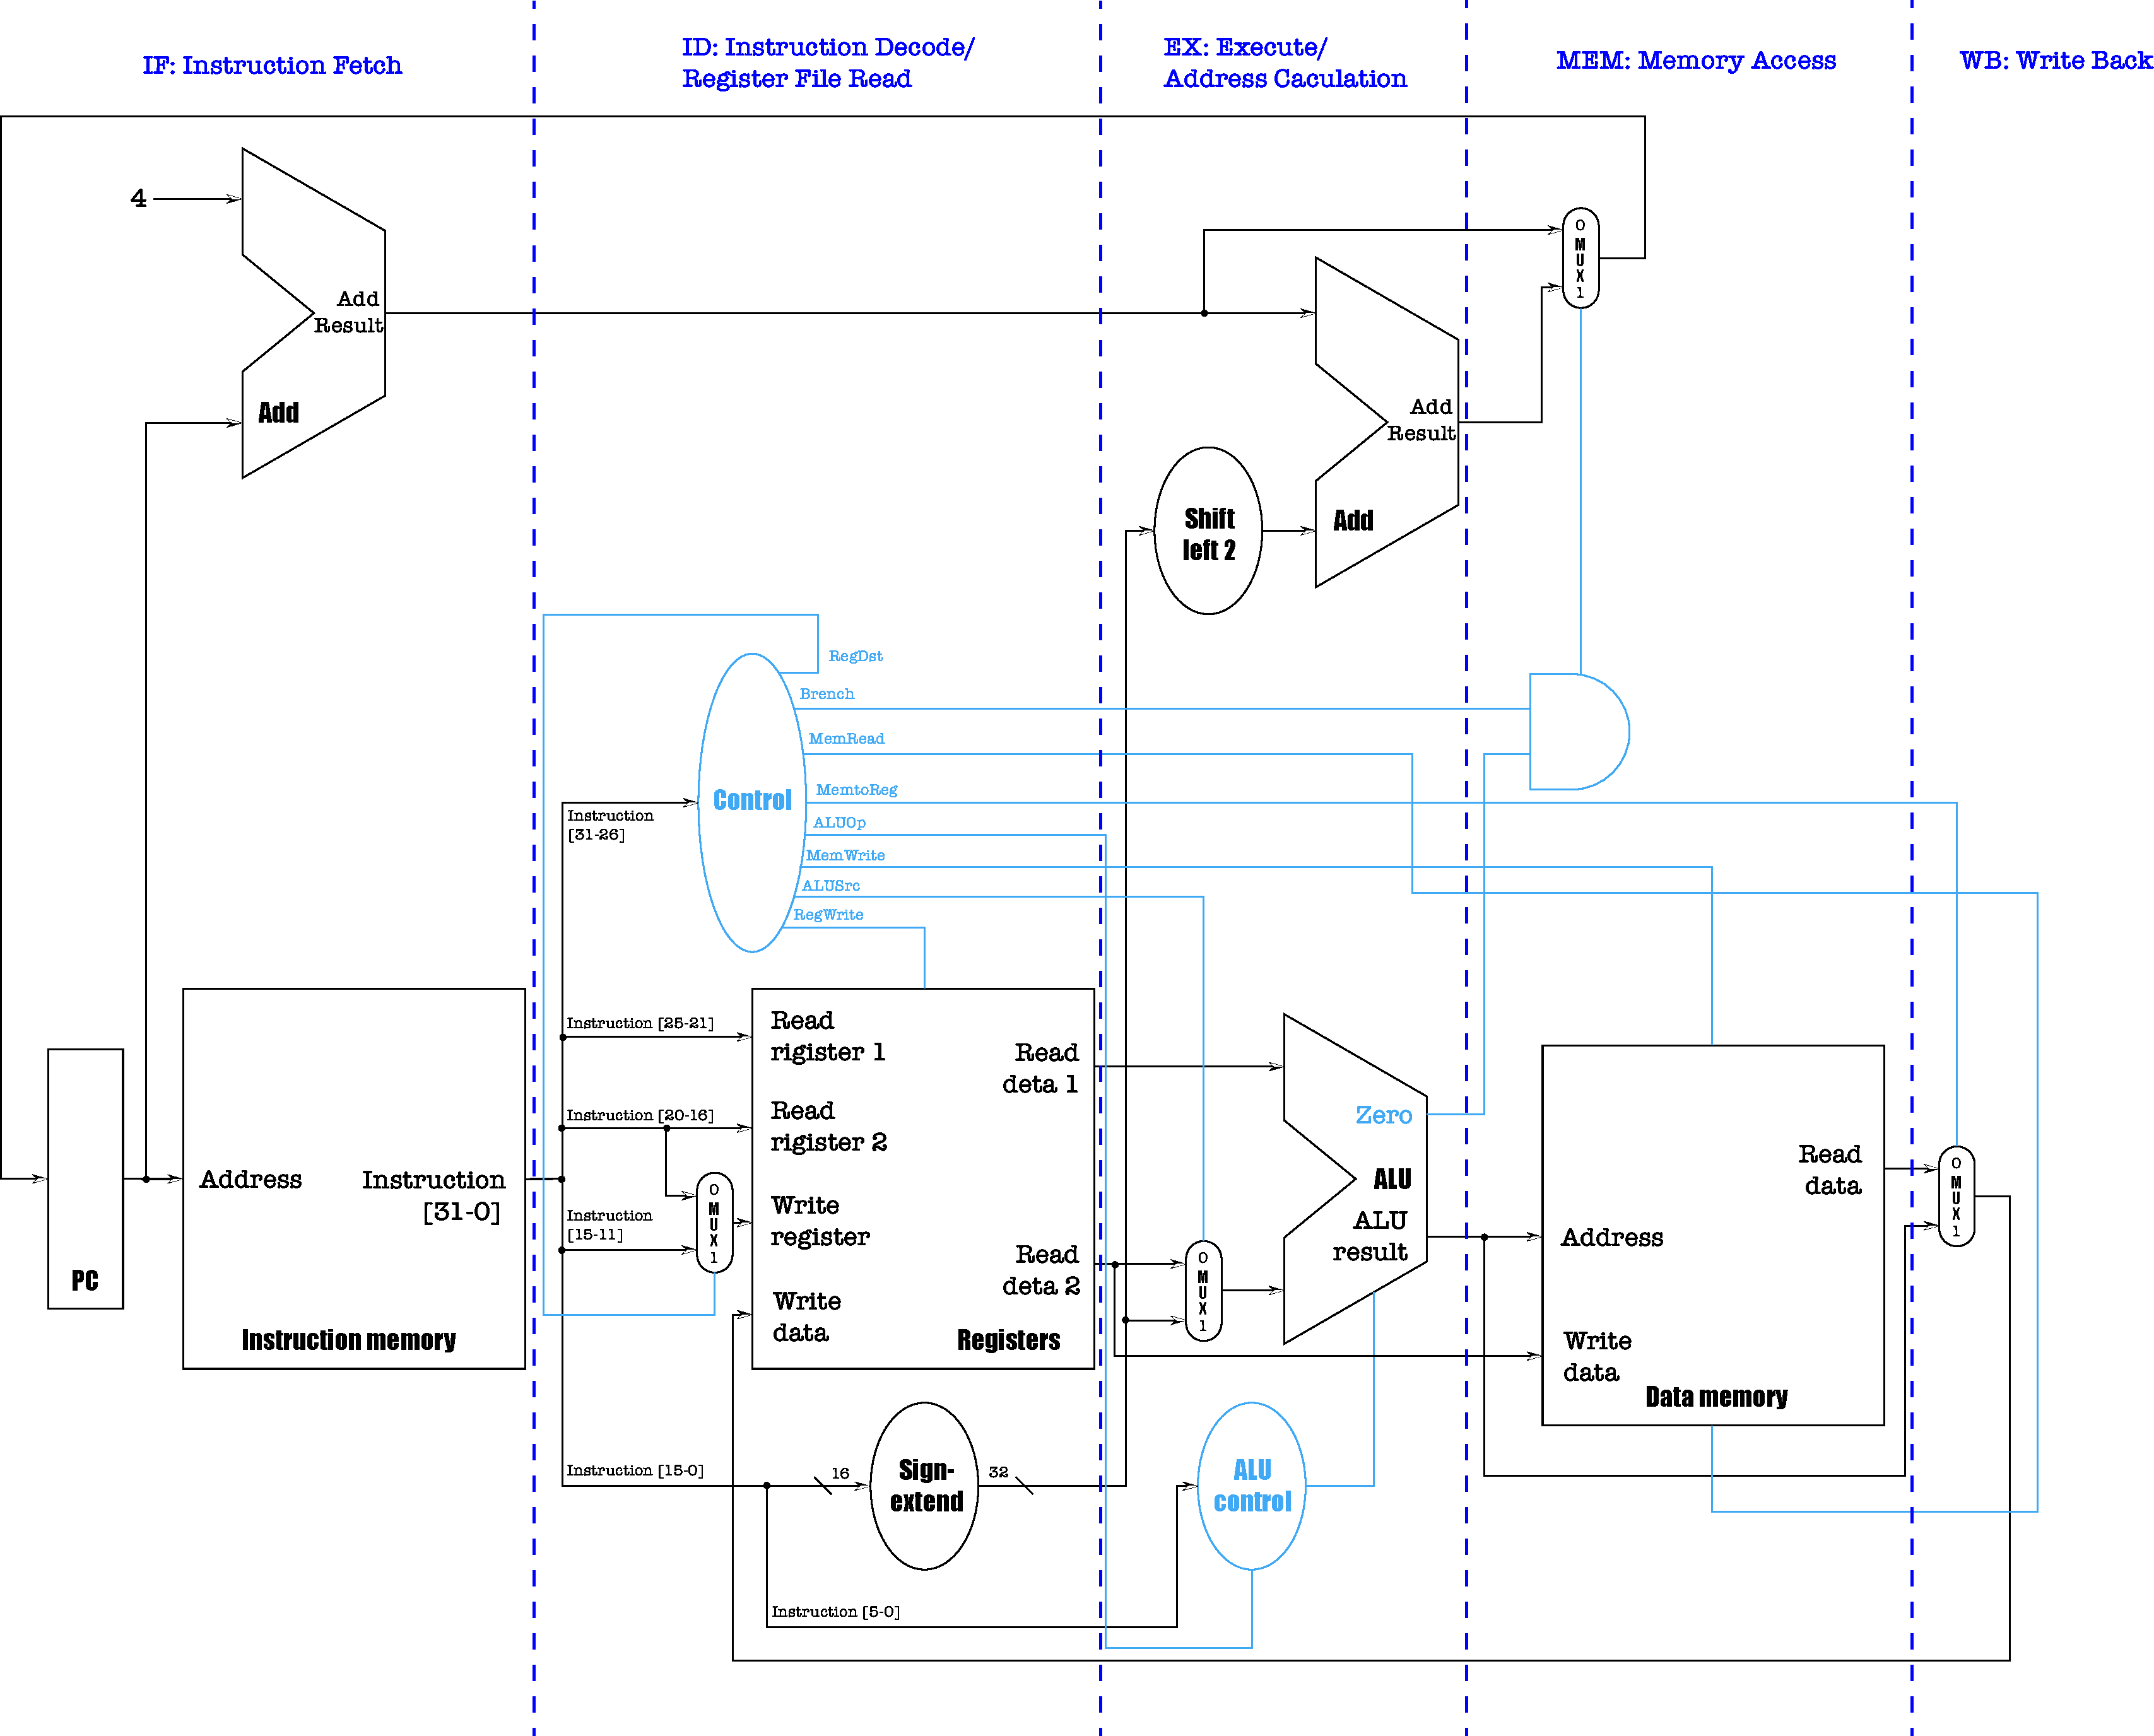
\includegraphics[scale=.2]{img/figure36.pdf}
\end{figure}
\subsection{单周期和流水线}
单周期指的是指令以串行的方式执行, 而流水线就是指令以并行的方式执行. \par
单周期每一个指令的时间相同, 而流水线每一个步骤的时间相同. 这是什么意思呢? 假设我们现在要执行\verb|3|次\verb|lw|指令, 先看\verb|lw|指令内部每一个步骤花的时间:
\begin{table}[H]
\centering
\begin{tabularx}{\textwidth}{|Z|Z|Z|Z|Z|Z|}
\hline
\textbf{Instr} & \textbf{IF} & \textbf{Reg Read} & \textbf{ALU} & \textbf{MEM} & \textbf{Reg Write} \\ \hline
lw & 200ps & 100ps & 200ps & 200ps & 100ps \\
\hline
\end{tabularx}
\end{table}
根据单周期和流水线的不同, 我们画出以下的以时间为轴的过程图:
\begin{figure}[H]
\centering
\begin{subfigure}{\textwidth}
\centering
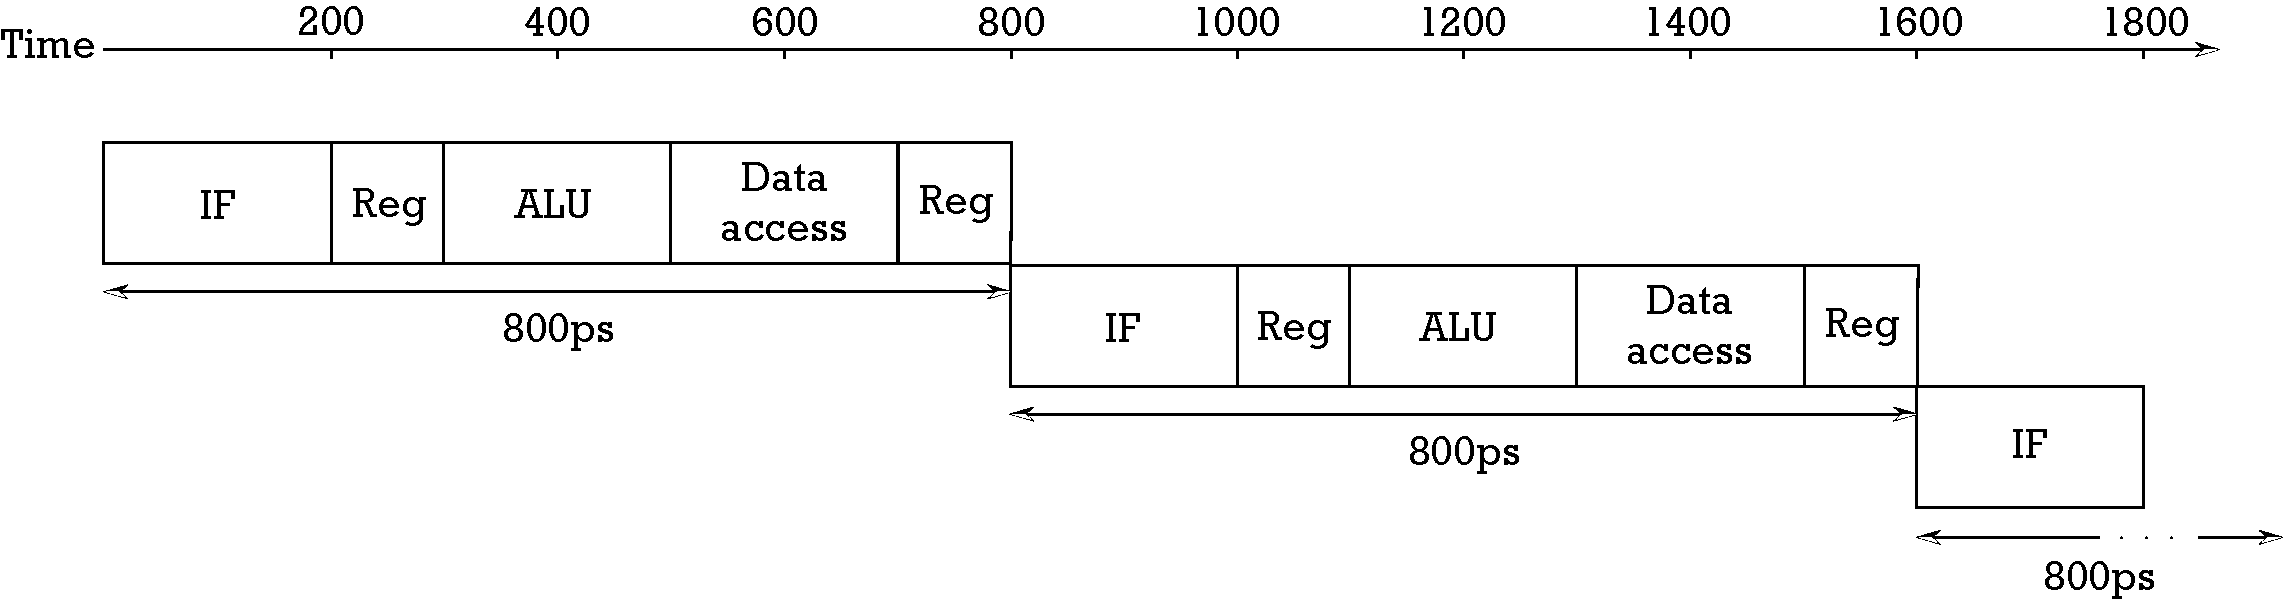
\includegraphics[scale=.4]{img/figure38.pdf}
\caption{单周期}
\end{subfigure}\vspace{2em}
\begin{subfigure}{\textwidth}
\centering
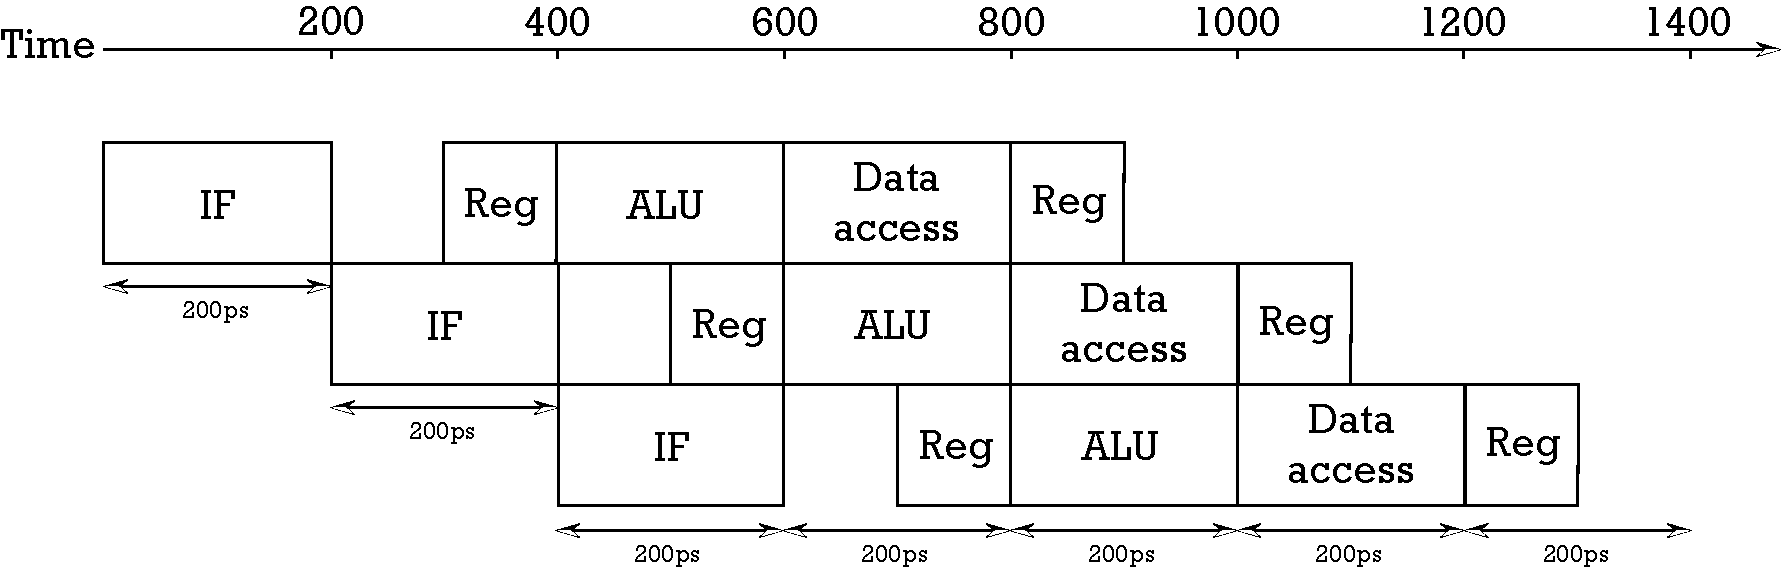
\includegraphics[scale=.4]{img/figure39.pdf}
\caption{流水线}
\end{subfigure}
\end{figure}
假设对寄存器的读操作发生在时钟周期的后半部分, 写操作发生在前半部分. 可以看到, 流水线的时钟周期受限于最慢的处理步骤, 时间为\verb|200ps|, 所以所有的流水级(\verb|Stage|)都是\verb|200ps|. 而单周期的每一个指令都是\verb|800ps|.\par
加速比\verb|=3*800/(800+3*200)|$ \symtt{\approx} $\verb|1.7|, 如果指令数量足够多的化, 如再增加\verb|1000000|条, 则加速比\verb|=1000000*|\\\verb|800/(800+1000000*200)|$ \symtt{\approx} $\verb|4|. 没有达到\verb|5|, 理想情况下可以达到.\par 
\paragraph{总结}~{} 
\begin{itemize}
\item 流水线可以改善吞吐率
\item 有些指令的有些时钟周期是浪费的
\item \verb|加速比=单周期指令的执行时间/流水线指令的执行时间|$ \symtt{\approx} $\verb|流水线级数(理想情况)|
\item 单挑指令的执行时间相比于单周期不减少, 有时反而会增加(如上述流水线中单条指令的执行时间为\verb|1000ps|)
\end{itemize}
\subsection{冒险}
流水线线还有这样一种情况, 在下一个时钟周期中下一条指令不能执行. 这种情况称为冒险. 下面介绍三种冒险:
\begin{itemize}
\item 结构冒险 \par 由于硬件结构导致的冒险, 两条指令没法同时使用一块硬件 \par (如两条指令在不同的阶段需要同时访问相同的寄存器)
\item 数据冒险 \par 下一条指令需要数据, 上一条指令还再计算中.
\begin{lstlisting}
add $s0, $t0, $t1
sub $t2 $s0 $t3
sub指令执行到ID的时候, add指令只执行到EX阶段, 需要等到add指令执行完WB才能把结果写回$s0中
\end{lstlisting}
\item 控制冒险(分支冒险) \par 下一条指令取决于上一条分支指令的结果.
\end{itemize}
\subsubsection{流水线的图形表示}
\begin{figure}[H]
\centering
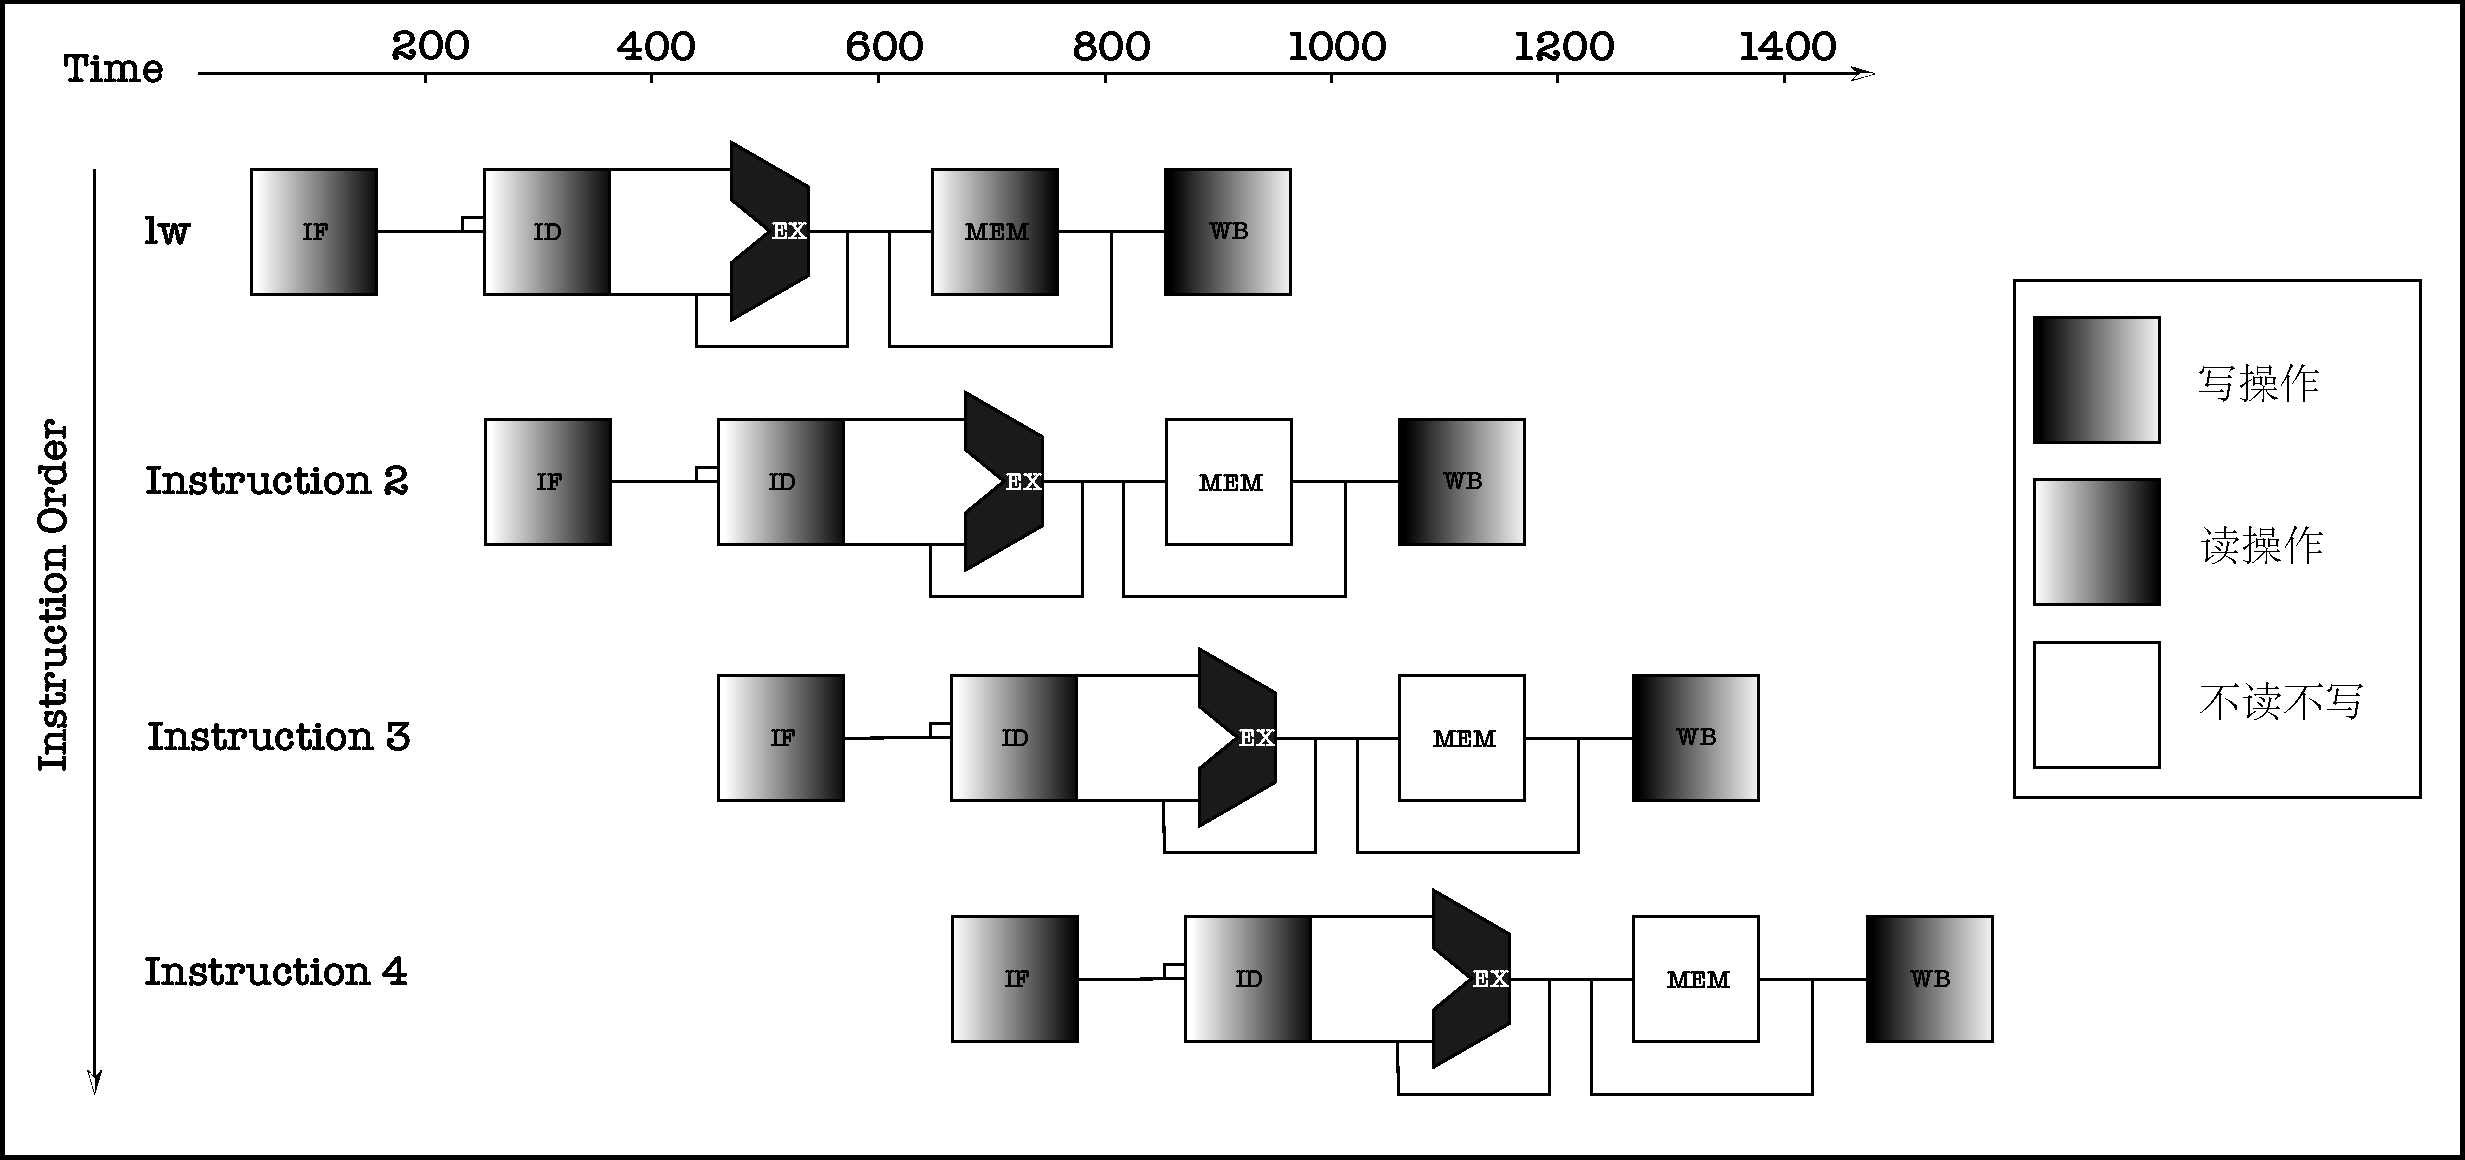
\includegraphics[scale=.4]{img/figure45.pdf}
\end{figure}
上图的方框含义:
\begin{itemize}
\item \verb|IF|: 表示取指阶段, 其外方框表示存储器, 右边的阴影表示读取存储器
\item \verb|ID|: 表示指令的译码或者寄存器堆的读取阶段, 其外方框表示要读取的寄存器堆, 右边的阴影表示读取寄存器堆
\item \verb|EX|: 表示指令的执行阶段, 其外边的图符表示\verb|ALU|, 阴影表示使用\verb|ALU|计算
\item \verb|MEM|: 表示存储器访问阶段, 其外放框表示存储器, 右边的阴影表示读取存储器
\item \verb|WB|: 表示写回阶段, 其外方框表示被写回的寄存器堆, 左边的阴影表示写入寄存器堆
\end{itemize}\par
\subsubsection{结构冒险}
结构冒险是由于两条指令没法使用同一个硬件.
\begin{figure}[H]
\centering
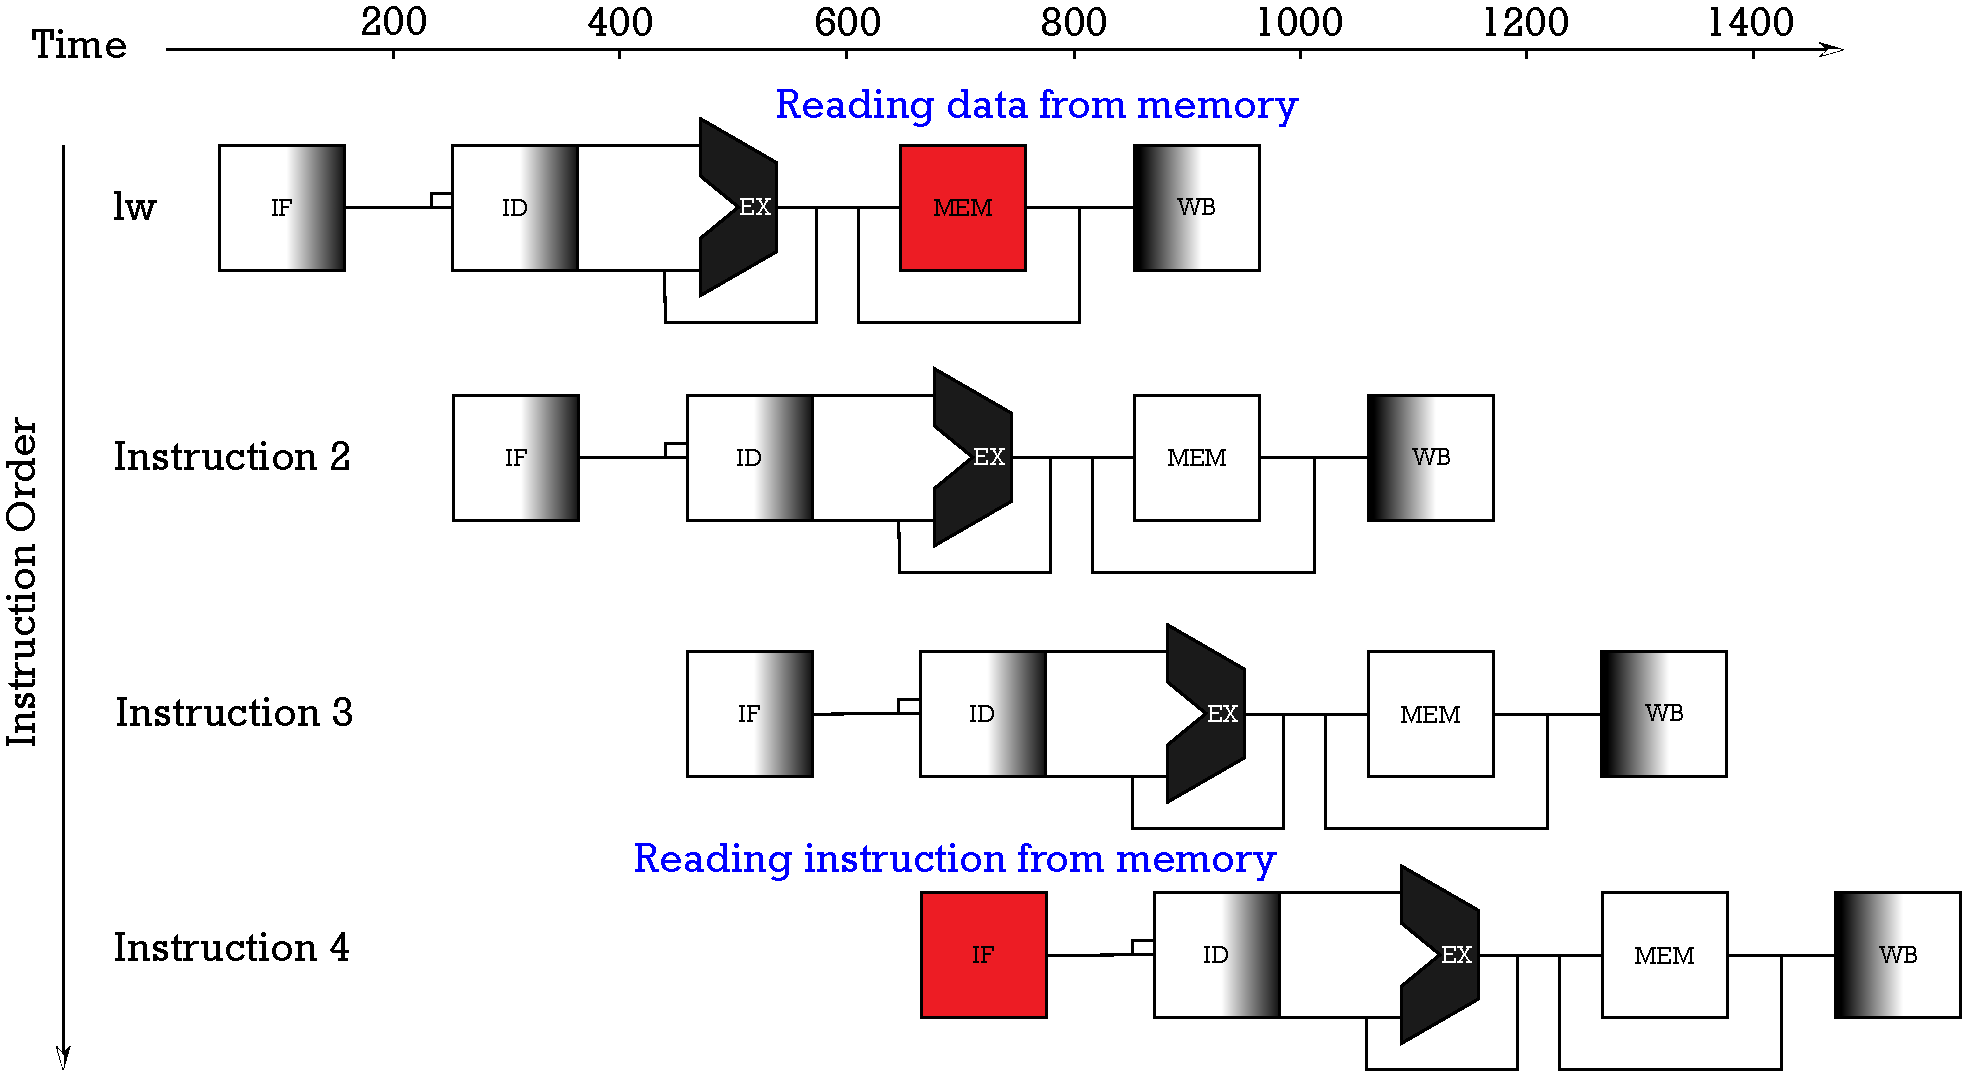
\includegraphics[scale=.4]{img/figure40.pdf}
\end{figure}
由于使用了同一个存储器, 第\verb|1|条指令在访问存储器的时候, 第\verb|4|条指令无法取指令. 进而就产生了结构冒险. 由于\verb|MIPS|是为流水线而设计的, 所以在设计之初就想到了这种问题, 所以就采取了一系列应对措施, 如将存储器拆分为指令存储器和数据存储器.
\subsubsection{数据冒险}
数据冒险是由于一条指令必须等待另一条指令的完成. 比较理想的情况是: 第\verb|1|条指令的\verb|WB|步骤在时钟周期的前半部分已经完成写操作, 第\verb|4|条指令的\verb|Reg Read|步骤在时钟周期的后半部分紧接着完成读操作, 如下图
\begin{figure}[H]
\centering
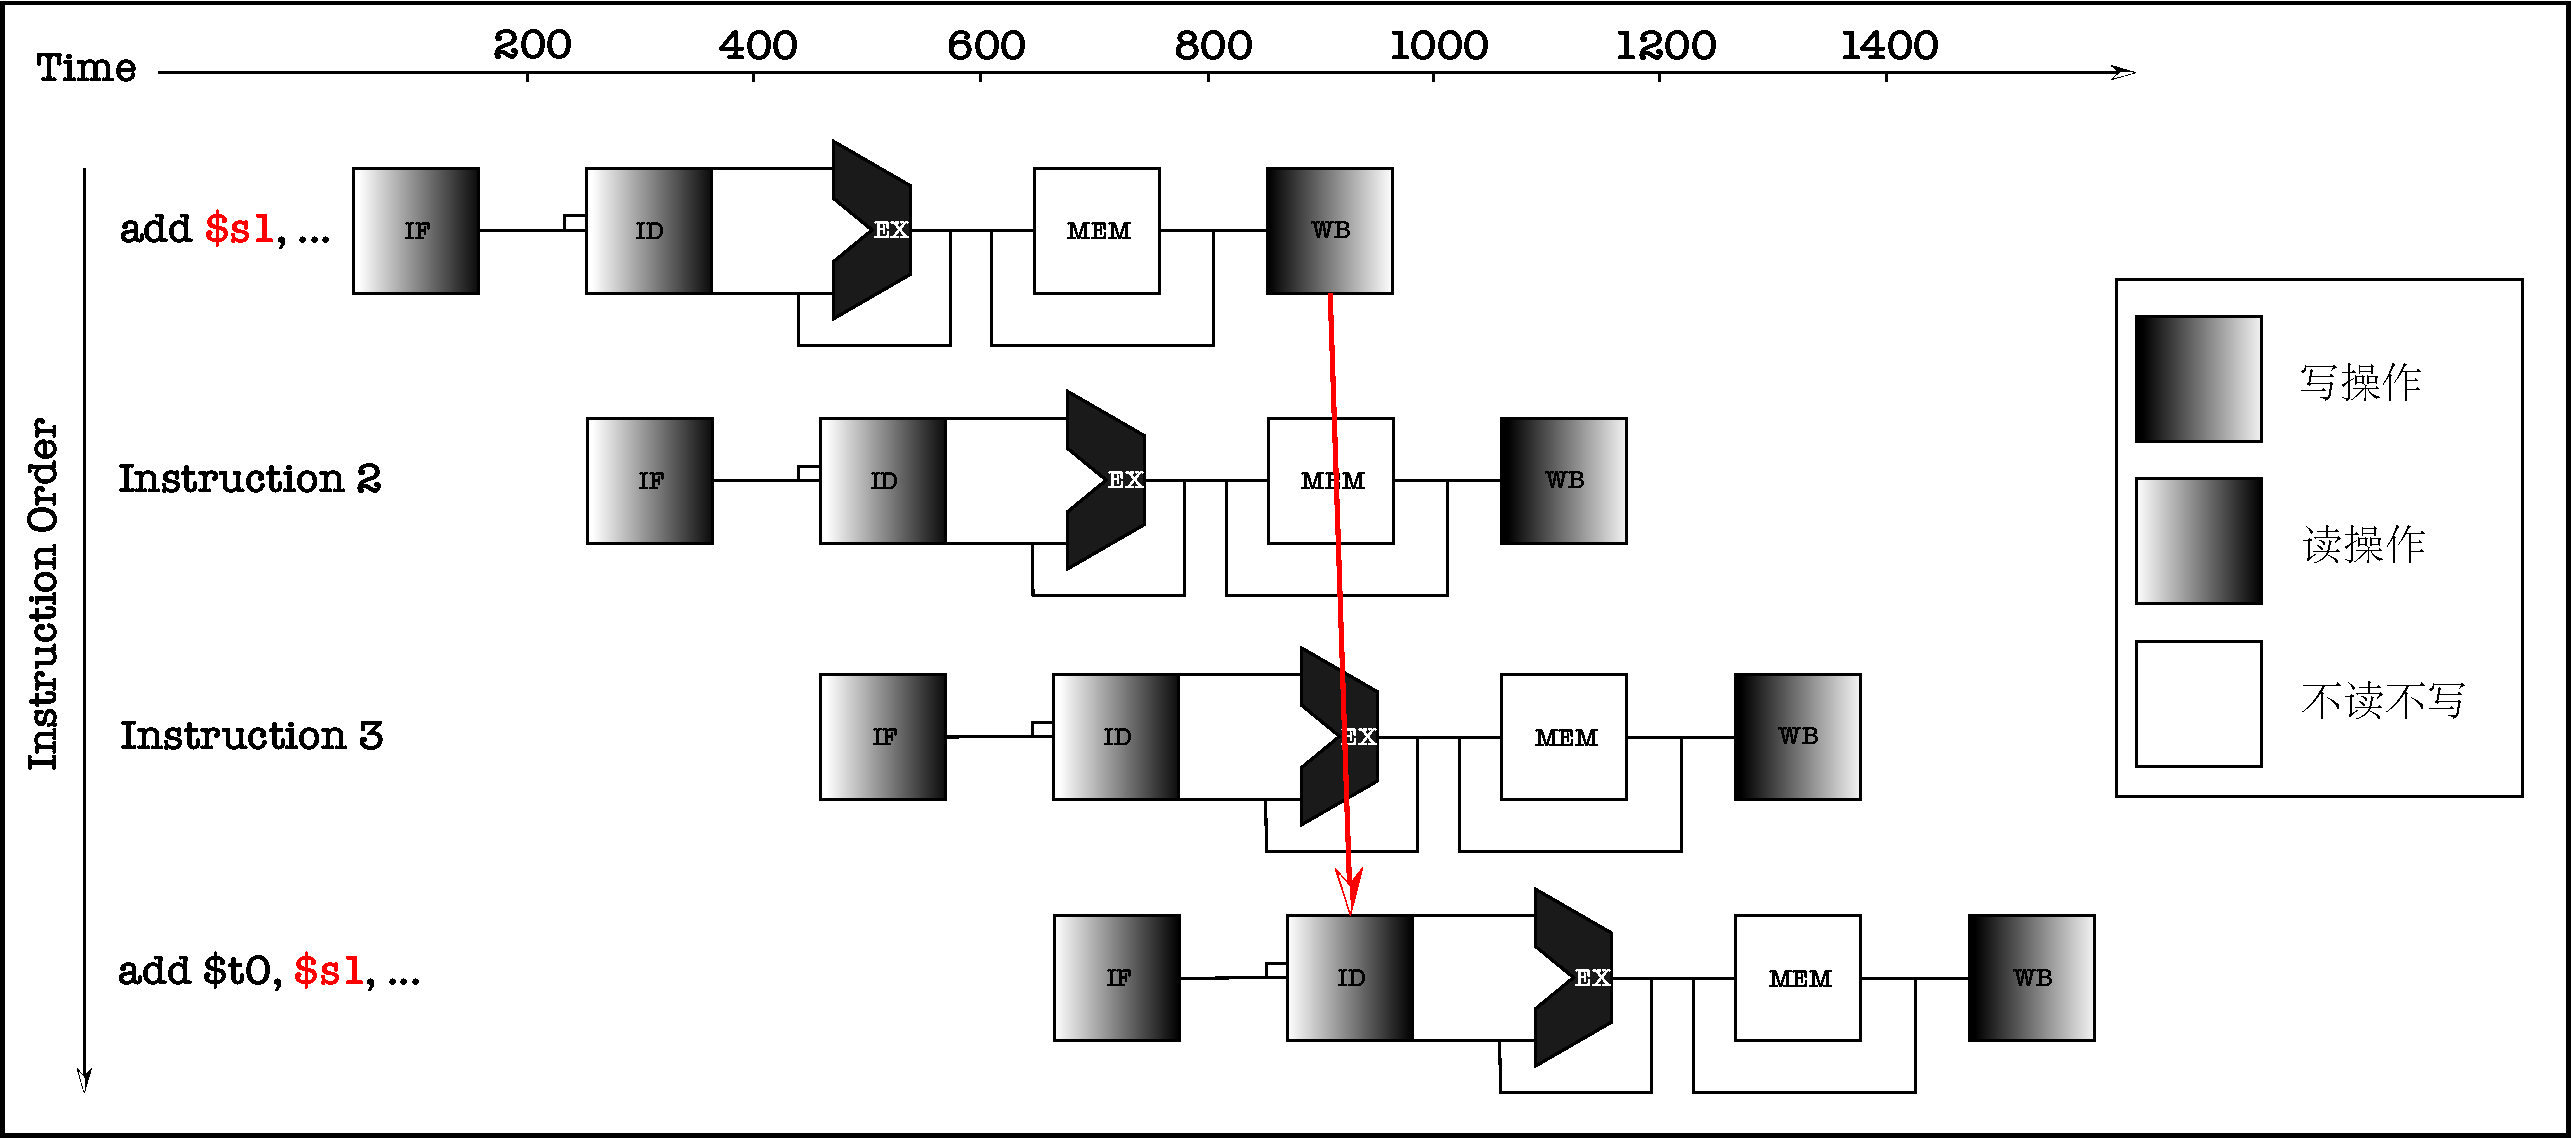
\includegraphics[scale=.4]{img/figure41.pdf}
\end{figure}
然而, 事实上, 这种情况几率较小, 大多数的情况下会造成阻塞:
\begin{figure}[H]
\centering
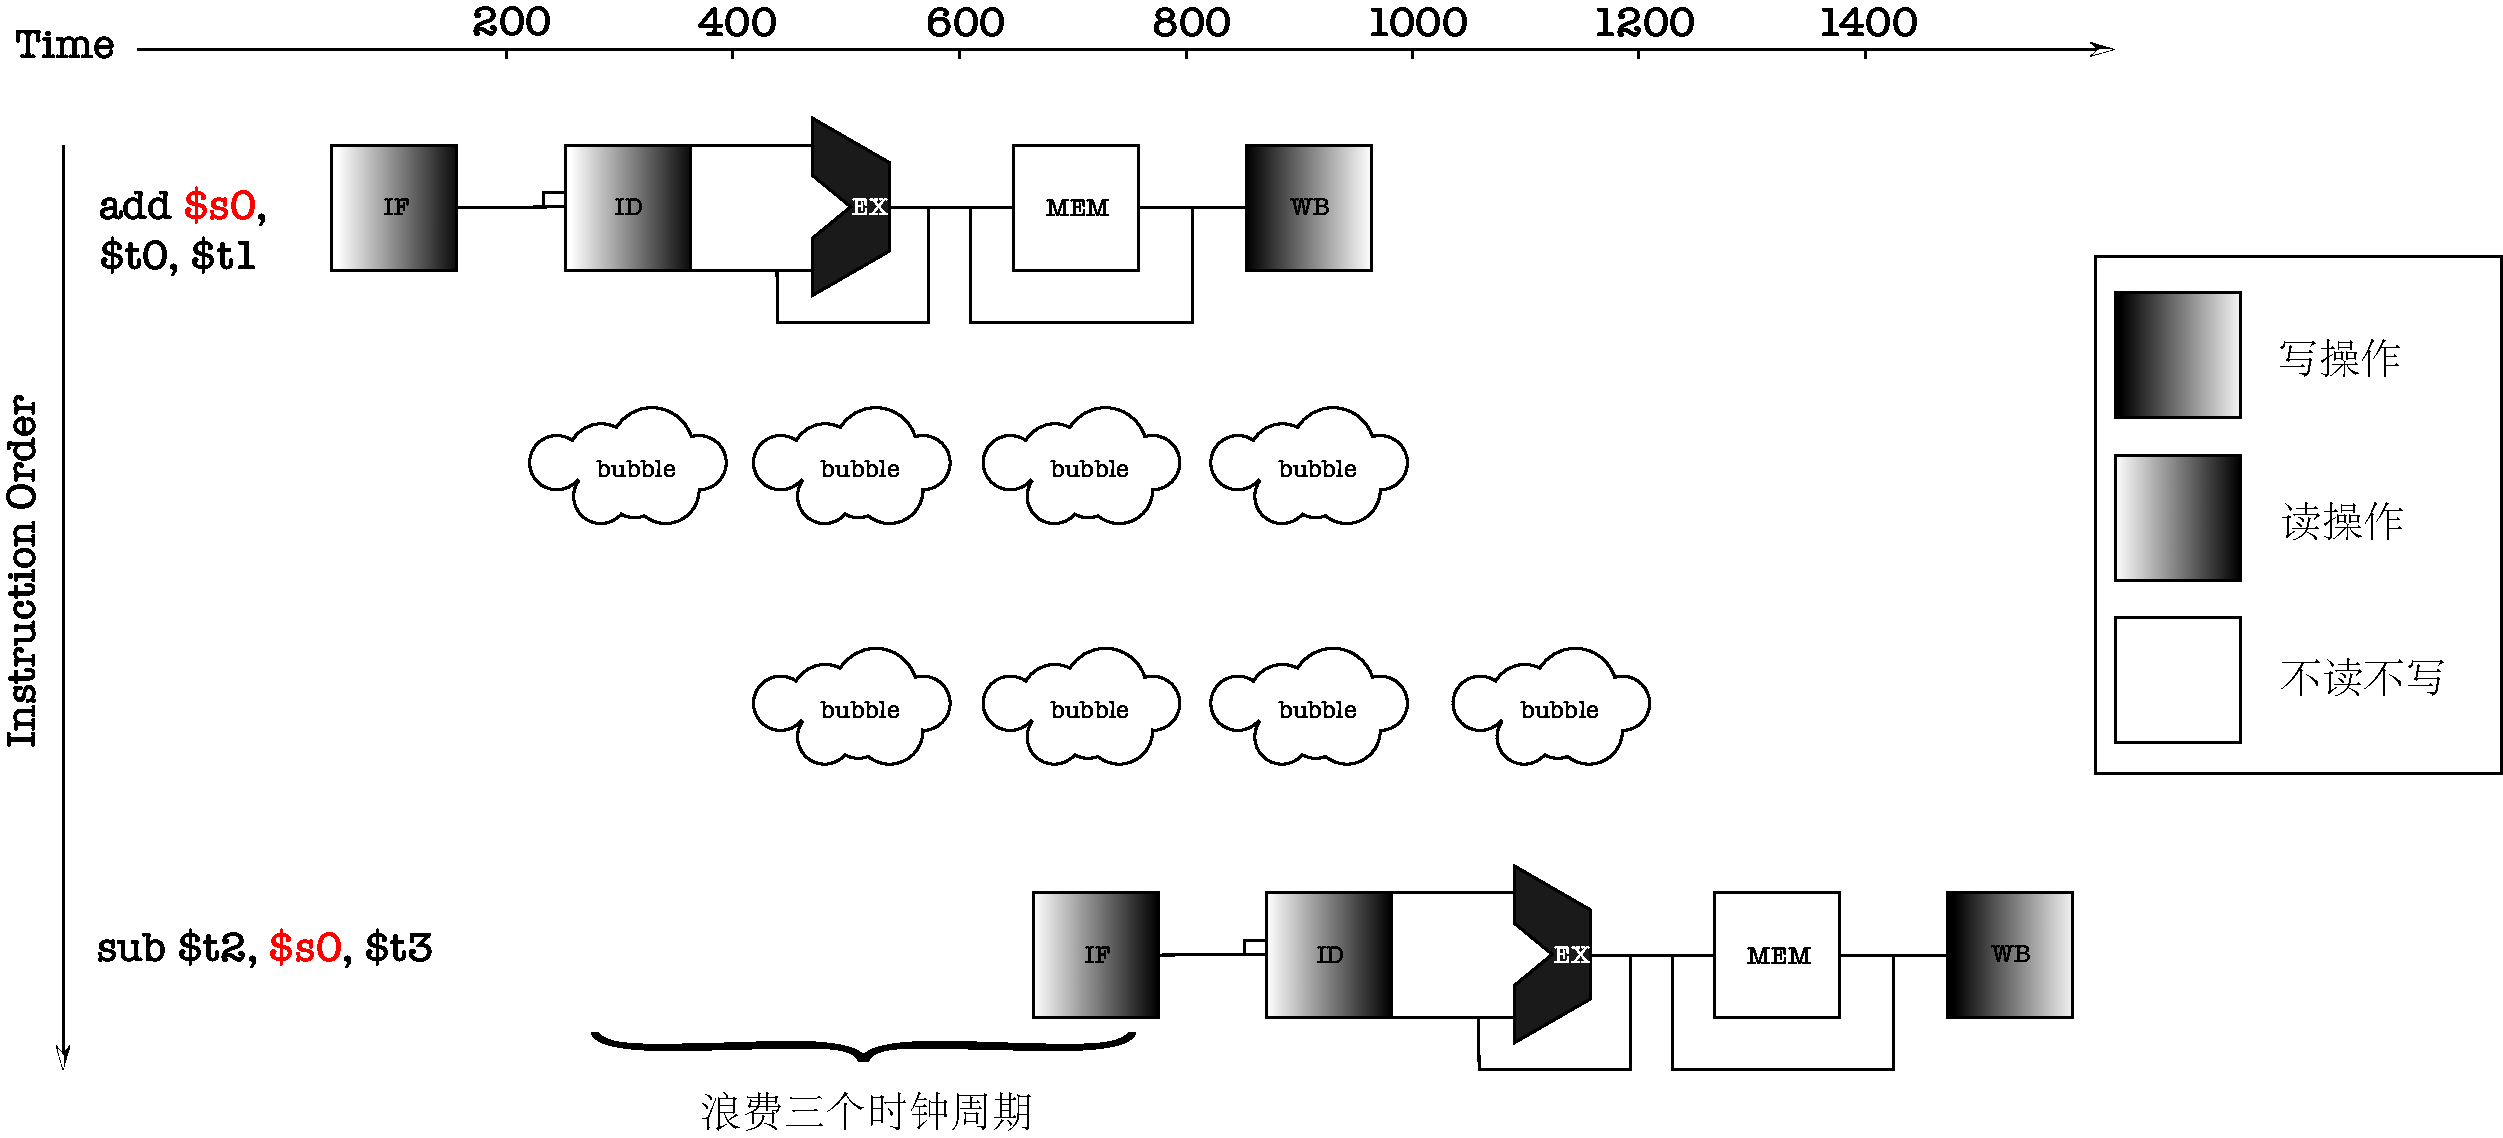
\includegraphics[scale=.4]{img/figure42.pdf}
\end{figure}
所以, 我们怎么解决这个问题呢?
\begin{figure}[H]
\centering
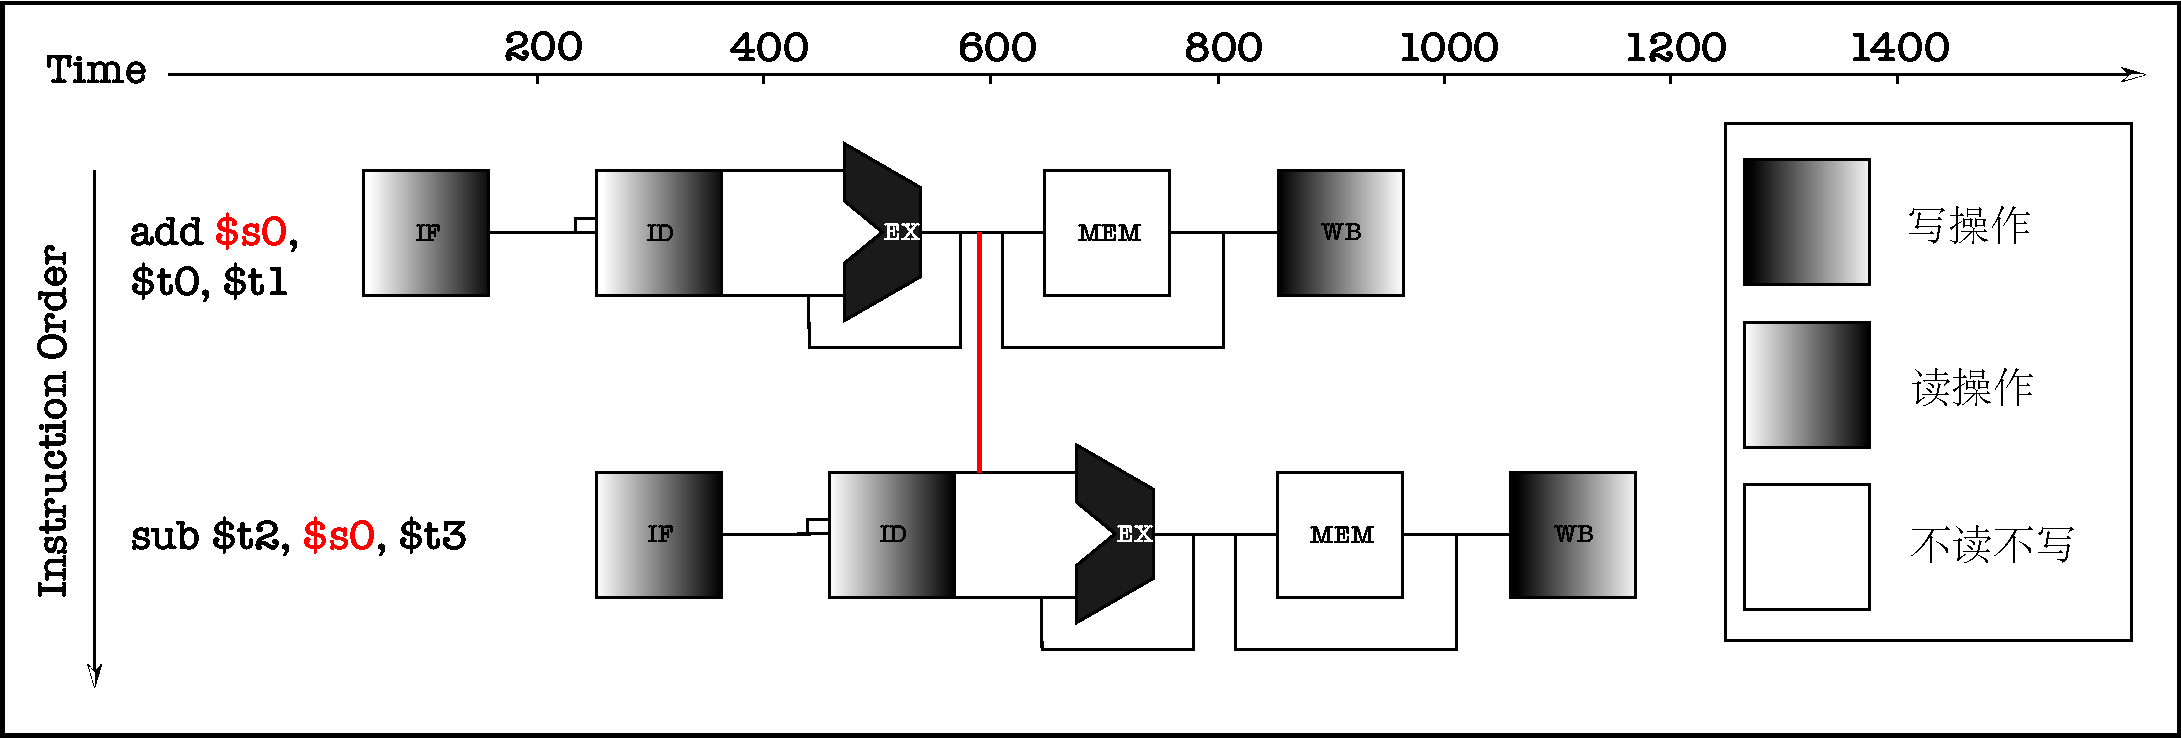
\includegraphics[scale=.4]{img/figure43.pdf}
\end{figure}
通过在数据通路中增加额外的硬件支持, 使前一条指令的\verb|ALU|一旦产生结果, 立即可以给后一条指令使用, 不必等到该数据存入指令中的目标寄存器. 上图中\verb|add|指令执行后的\verb|$s0|中的值作为\verb|sub|指令执行的输入的旁路连接.\par
转发并不能避免所有的流水线阻塞, 如{\heiti \textbf{取数-使用型数据冒险}}, 具体如图:
\begin{figure}[H]
\centering
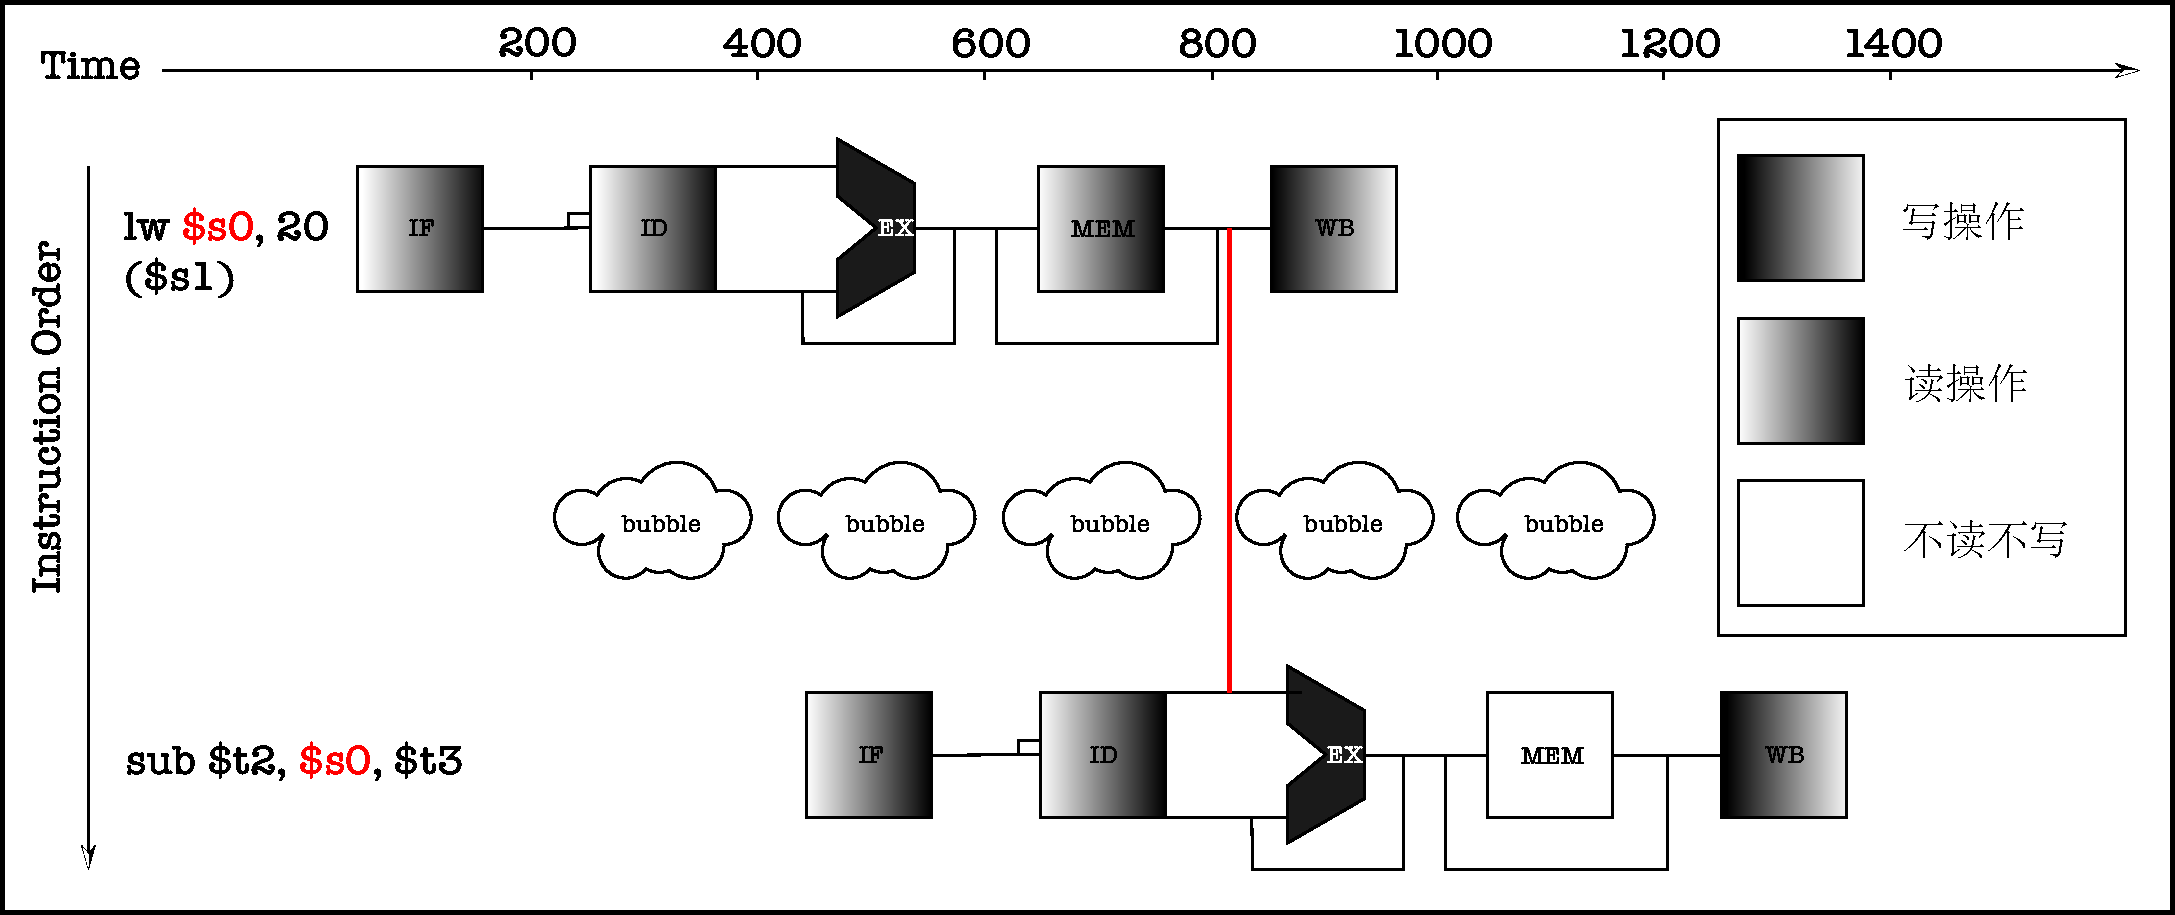
\includegraphics[scale=.4]{img/figure44.pdf}
\end{figure}\par
{\heiti \textbf{取数-使用型流水线}}是一种特殊的数据冒险, 指当装载指令要取的数还没取出的时候其他指令就要使用的情况, 流水线不得不阻塞一个步骤(正式的叫法是流水线阻塞, 又称气泡或者\verb|stall|).\par
所以, 解决这个问题的唯一方法就是重新构建代码以避免阻塞. 如以下代码:
\begin{lstlisting}
# BEFORE
lw $t1, 0($t0)
lw $t2, 4($t0)
add $t3, $t1, $t2 # stall
sw $t3, 12($t0)
lw $t4, 8($s0)
add $t5, $t1, $t4 # stall
sw $t5, 16($t0)
#AFTER
lw $t1, 0($t0)
lw $t2, 4($t0)
lw $t4, 8($t0)
add $t3, $t1, $t2
sw $t3, 12($t0)
add $t5, $t1, $t4
sw $t5, 16($t0)
\end{lstlisting}
\subsubsection{控制冒险}
根据流水线的规则, 当前指令处在\verb|ID|的时候, 下一条指令在\verb|IF|阶段. 但若当前指令是分支指令\verb|beq|, 则下一条指令是哪一条取决于分支指令的执行结果. 如下图就是由分支引起的控制冒险:
\begin{figure}[H]
\centering
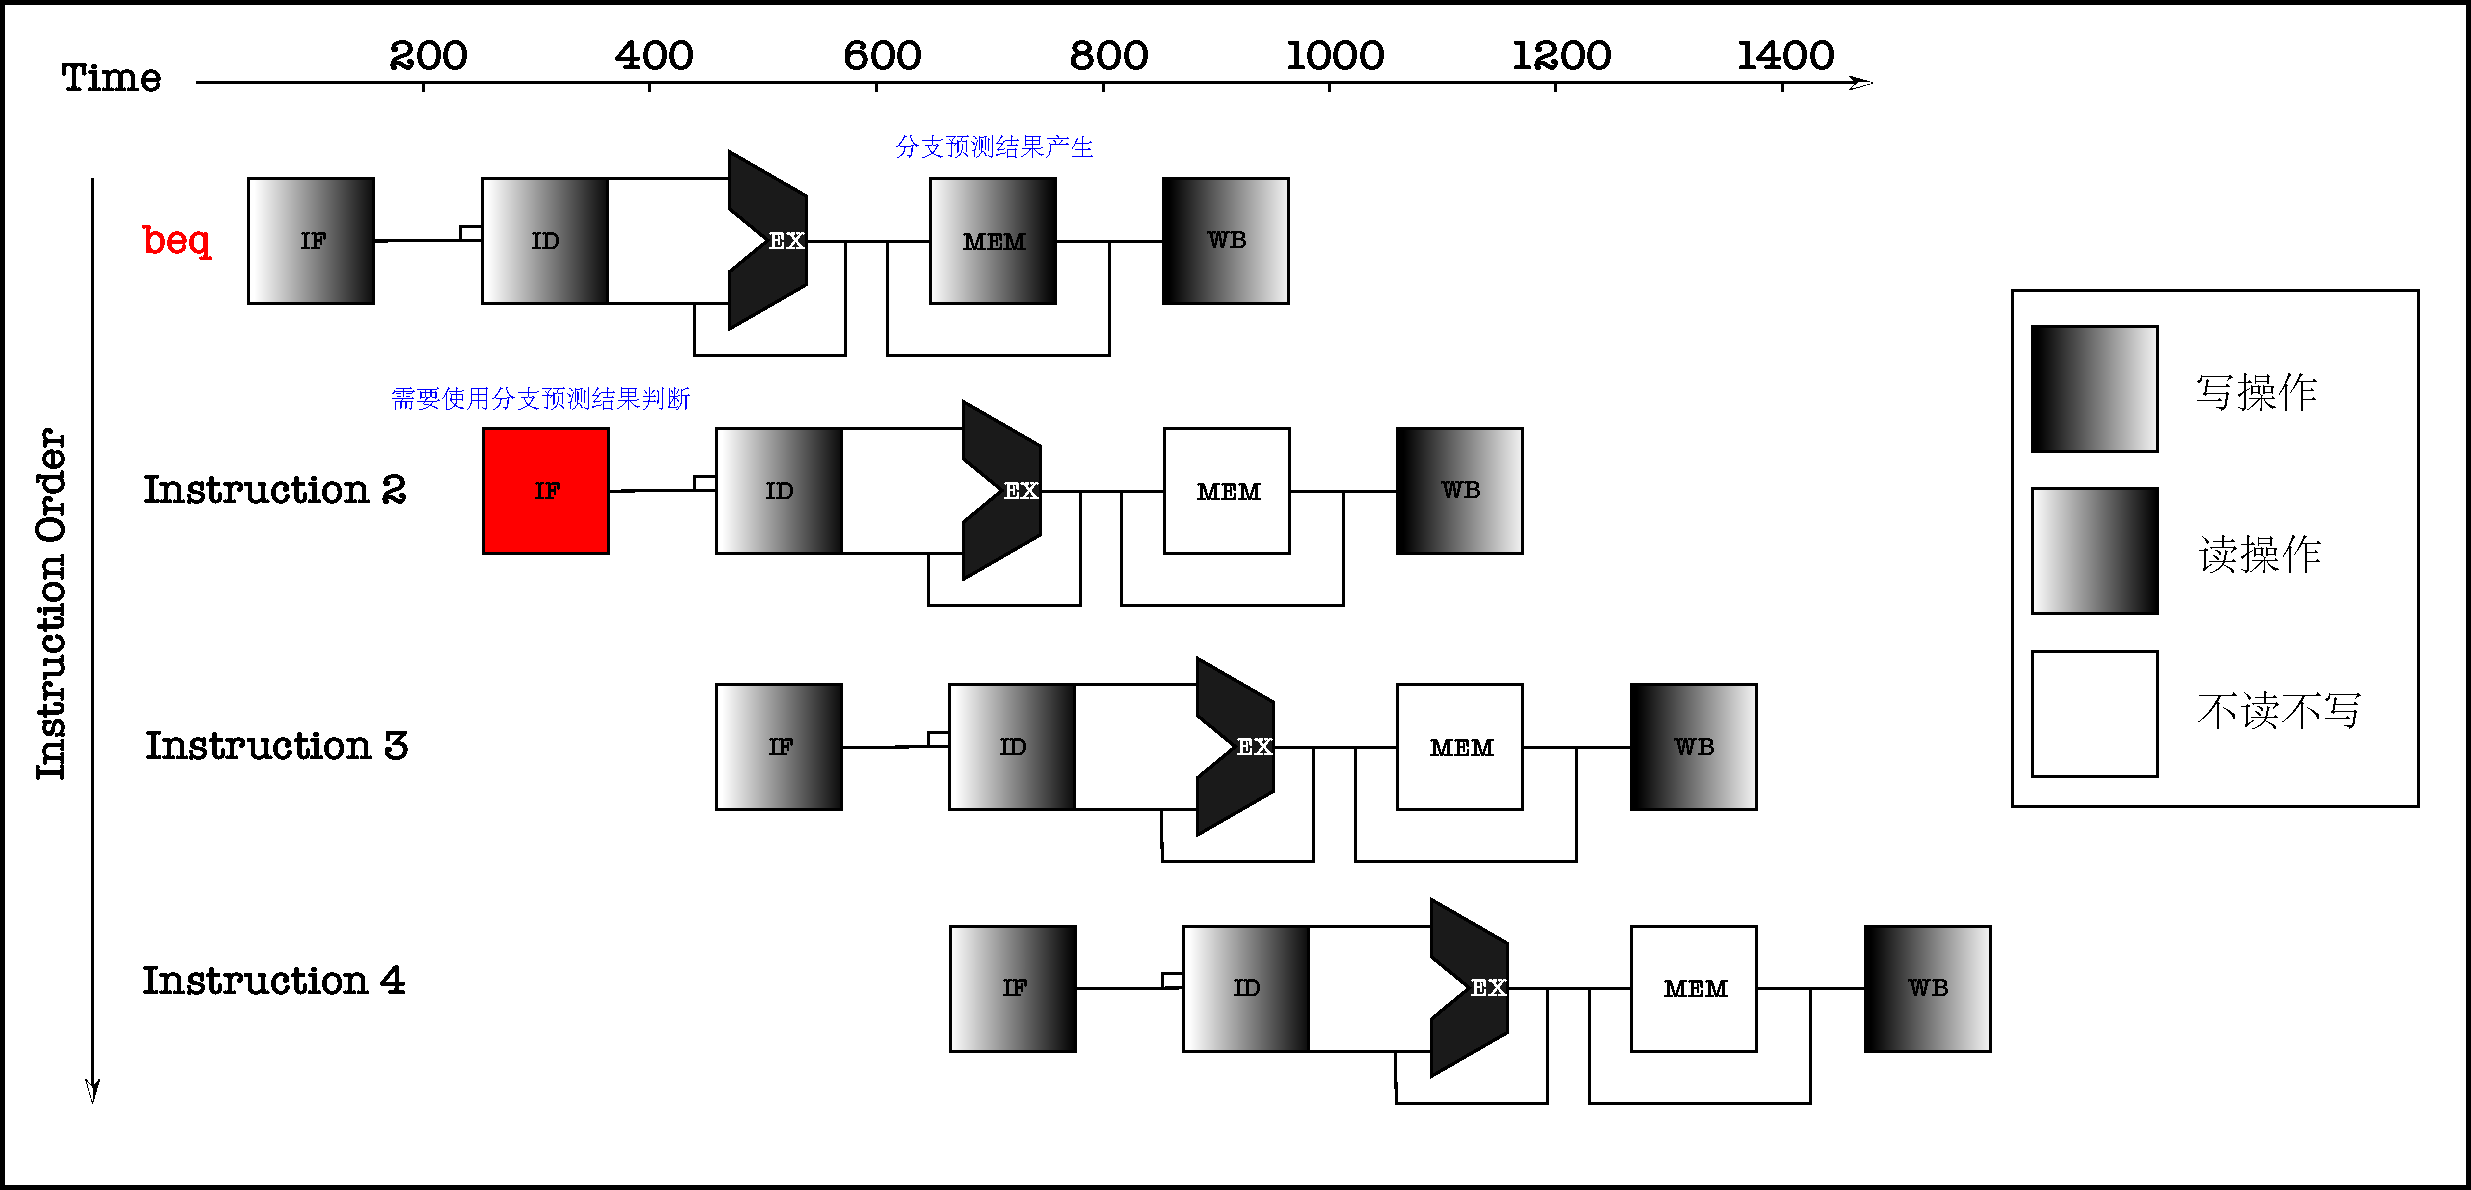
\includegraphics[scale=.4]{img/figure46.pdf}
\end{figure}
当\verb|Instruction2|处于\verb|IF|阶段时, 分支指令\verb|beq|还处于\verb|ID|阶段. \verb|beq|的\verb|MEM|阶段分支预测结果产生, 所以只有当\verb|beq|指令执行到\verb|WB|阶段的时候, 才能知道分支的结果. \par 解决上述问题有两种方法:
\begin{enumerate}
\item 阻塞 \par 等待分支指令的输出, 再取指. 正常情况下, 如果分支结果在\verb|MEM|阶段产生, 则需要阻塞三个周期, 如图:
\begin{figure}[H]
\centering
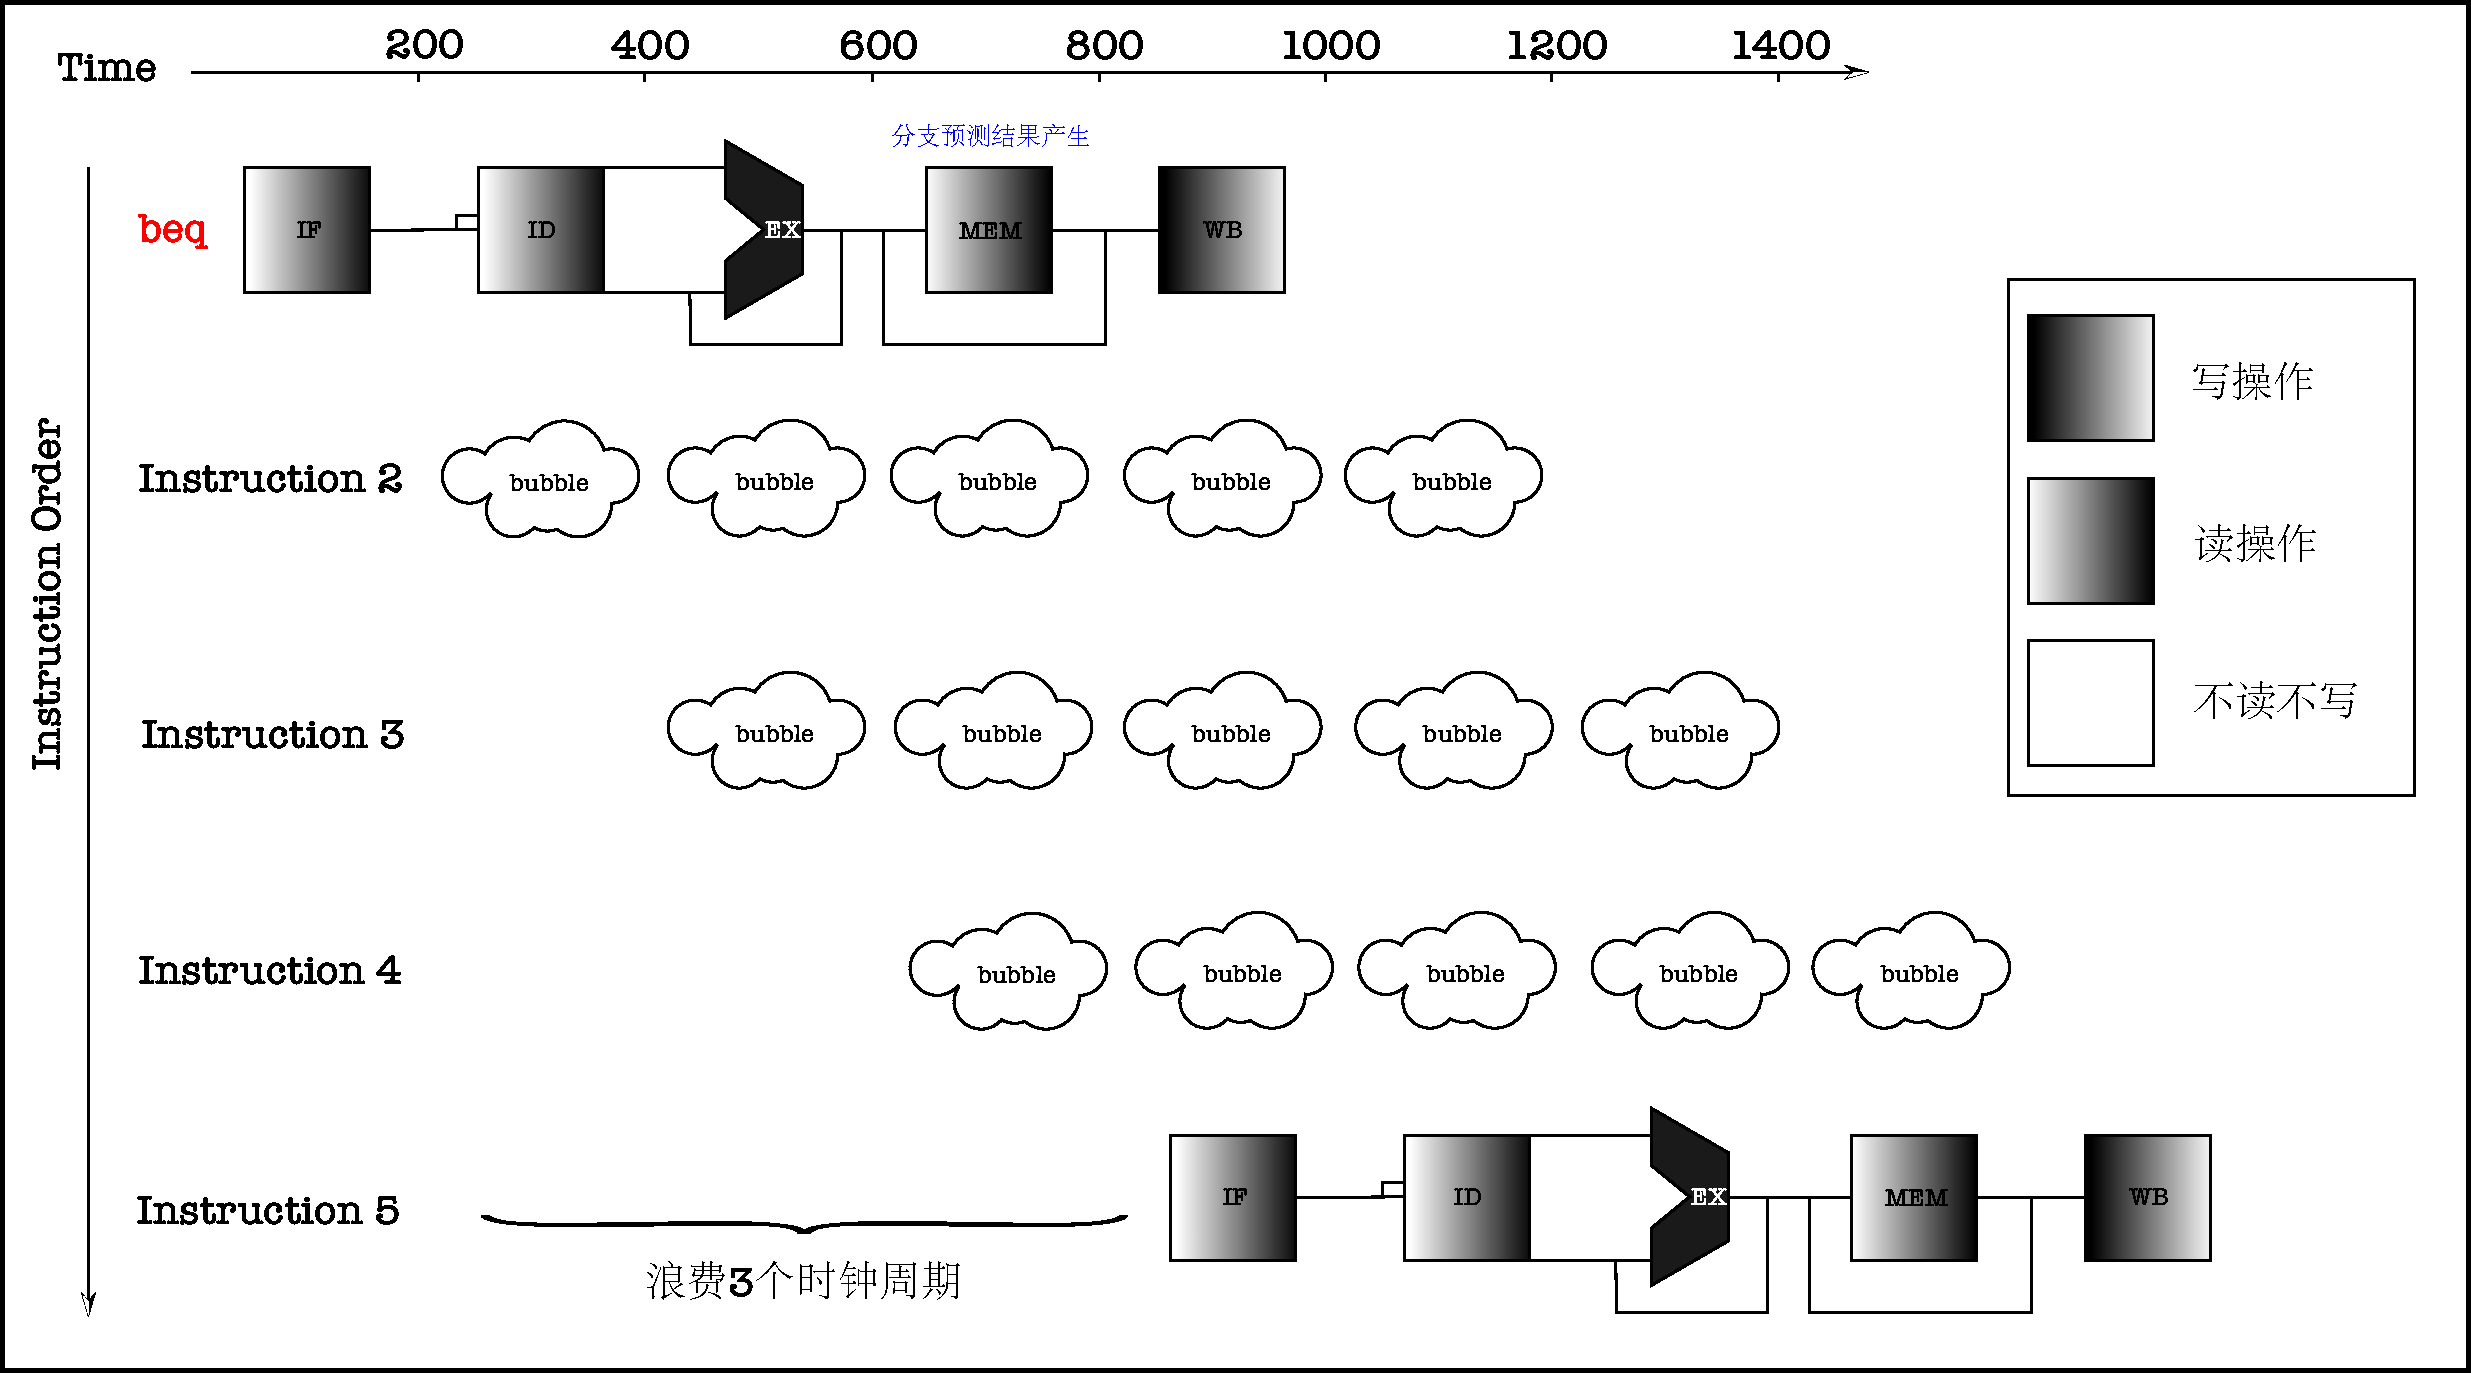
\includegraphics[scale=.4]{img/figure47.pdf}
\end{figure}
正常流水线下\verb|CPI|为\verb|1|, 即每一个时钟周期内就有一个指令完成, 假设\verb|beq|指令占所有指令的\verb|30%|, 则\verb|CPI|\\\verb|=1+0.3*3=1.9|, 大大降低了性能. 为此, 设计者又在\verb|ID|阶段增加了硬件, 使\verb|beq|指令在\verb|ID|阶段就能计算分支地址并更新\verb|PC|, 如图:
\begin{figure}[H]
\centering
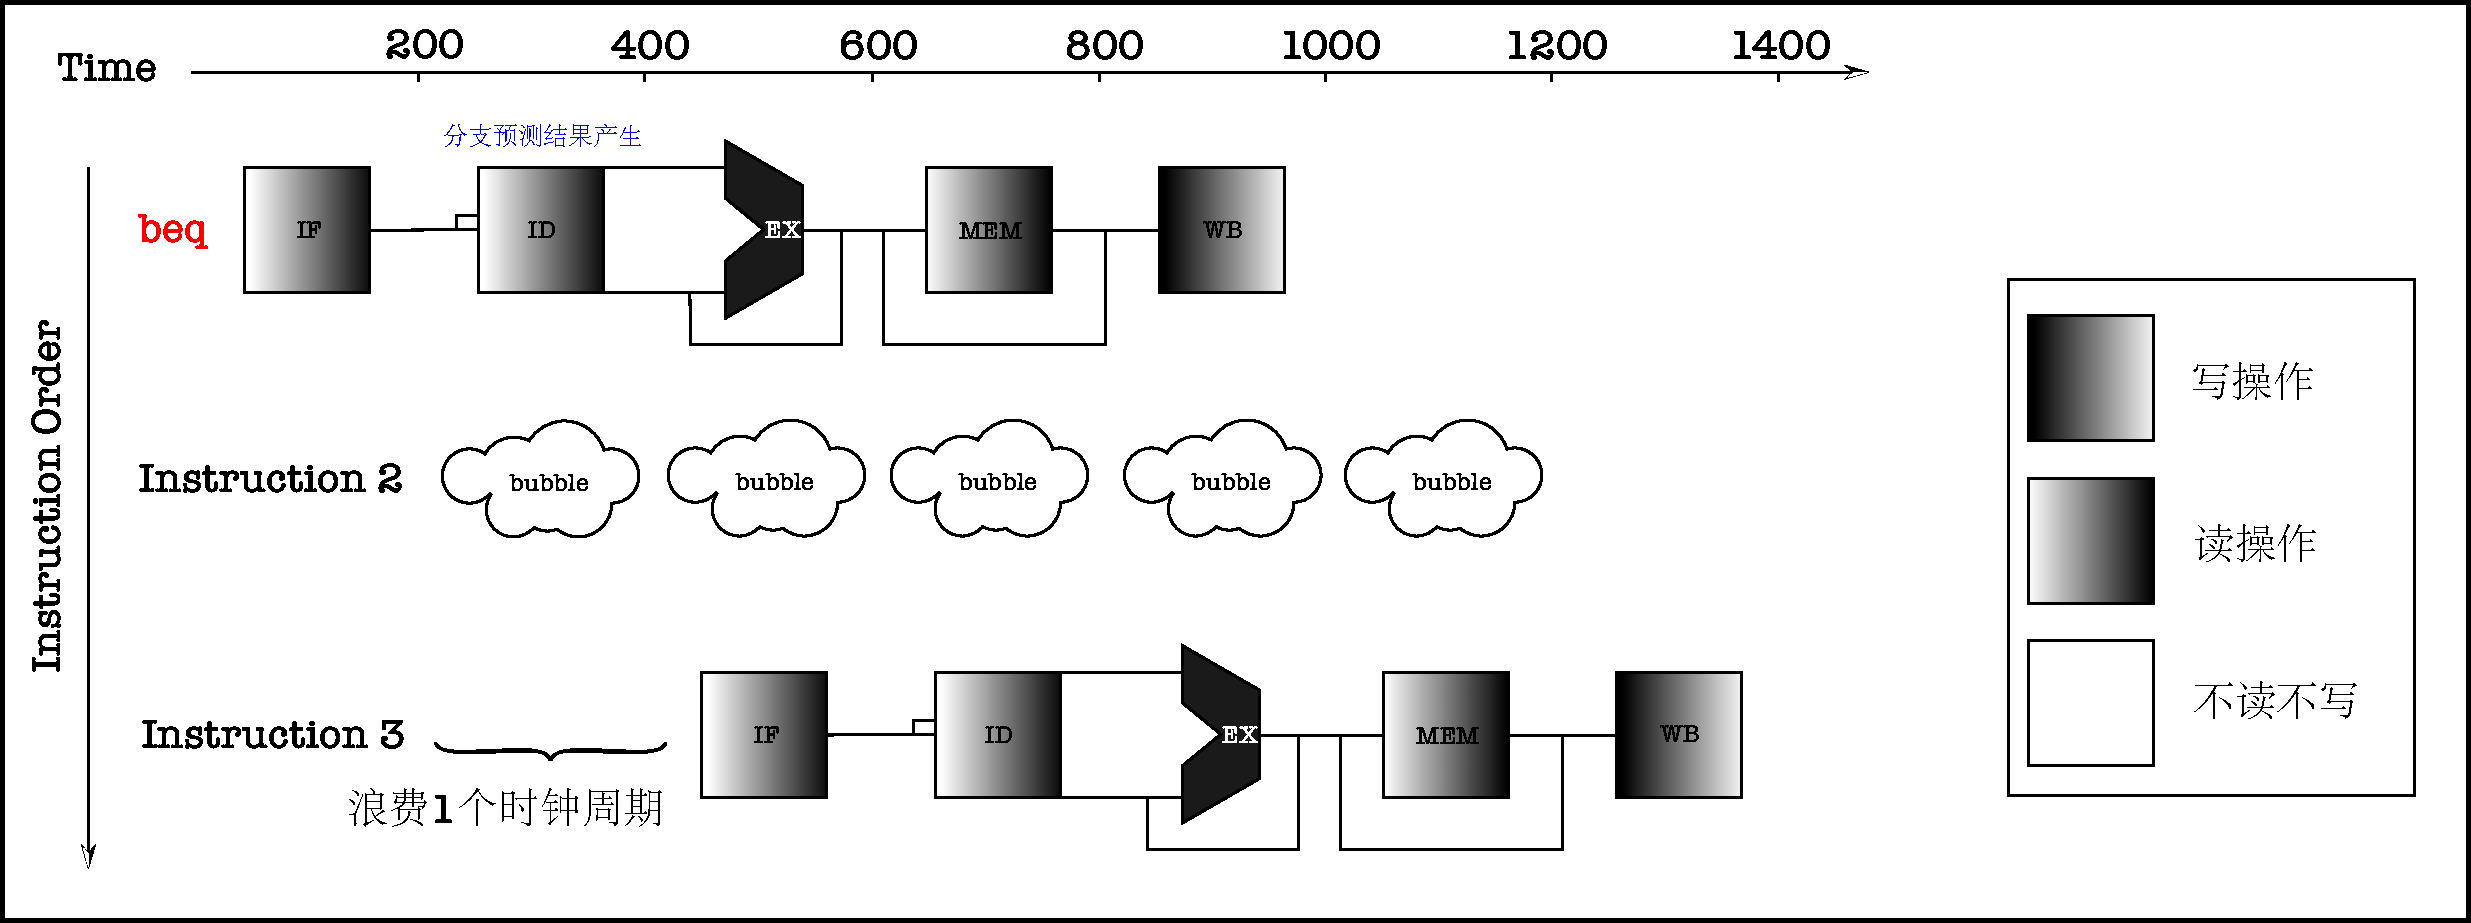
\includegraphics[scale=.4]{img/figure48.pdf}
\end{figure}
这种情况下, \verb|CPI=1+0.3*1=1.3|, 能改善性能, 但微乎其微.
\item 预测 \par 总是预测分支未发生, 当预测正确(分支未发生的时候), 流水线会全速地执行. 只有当分支发生时, 流水线才会阻塞.
\begin{figure}[H]
\centering
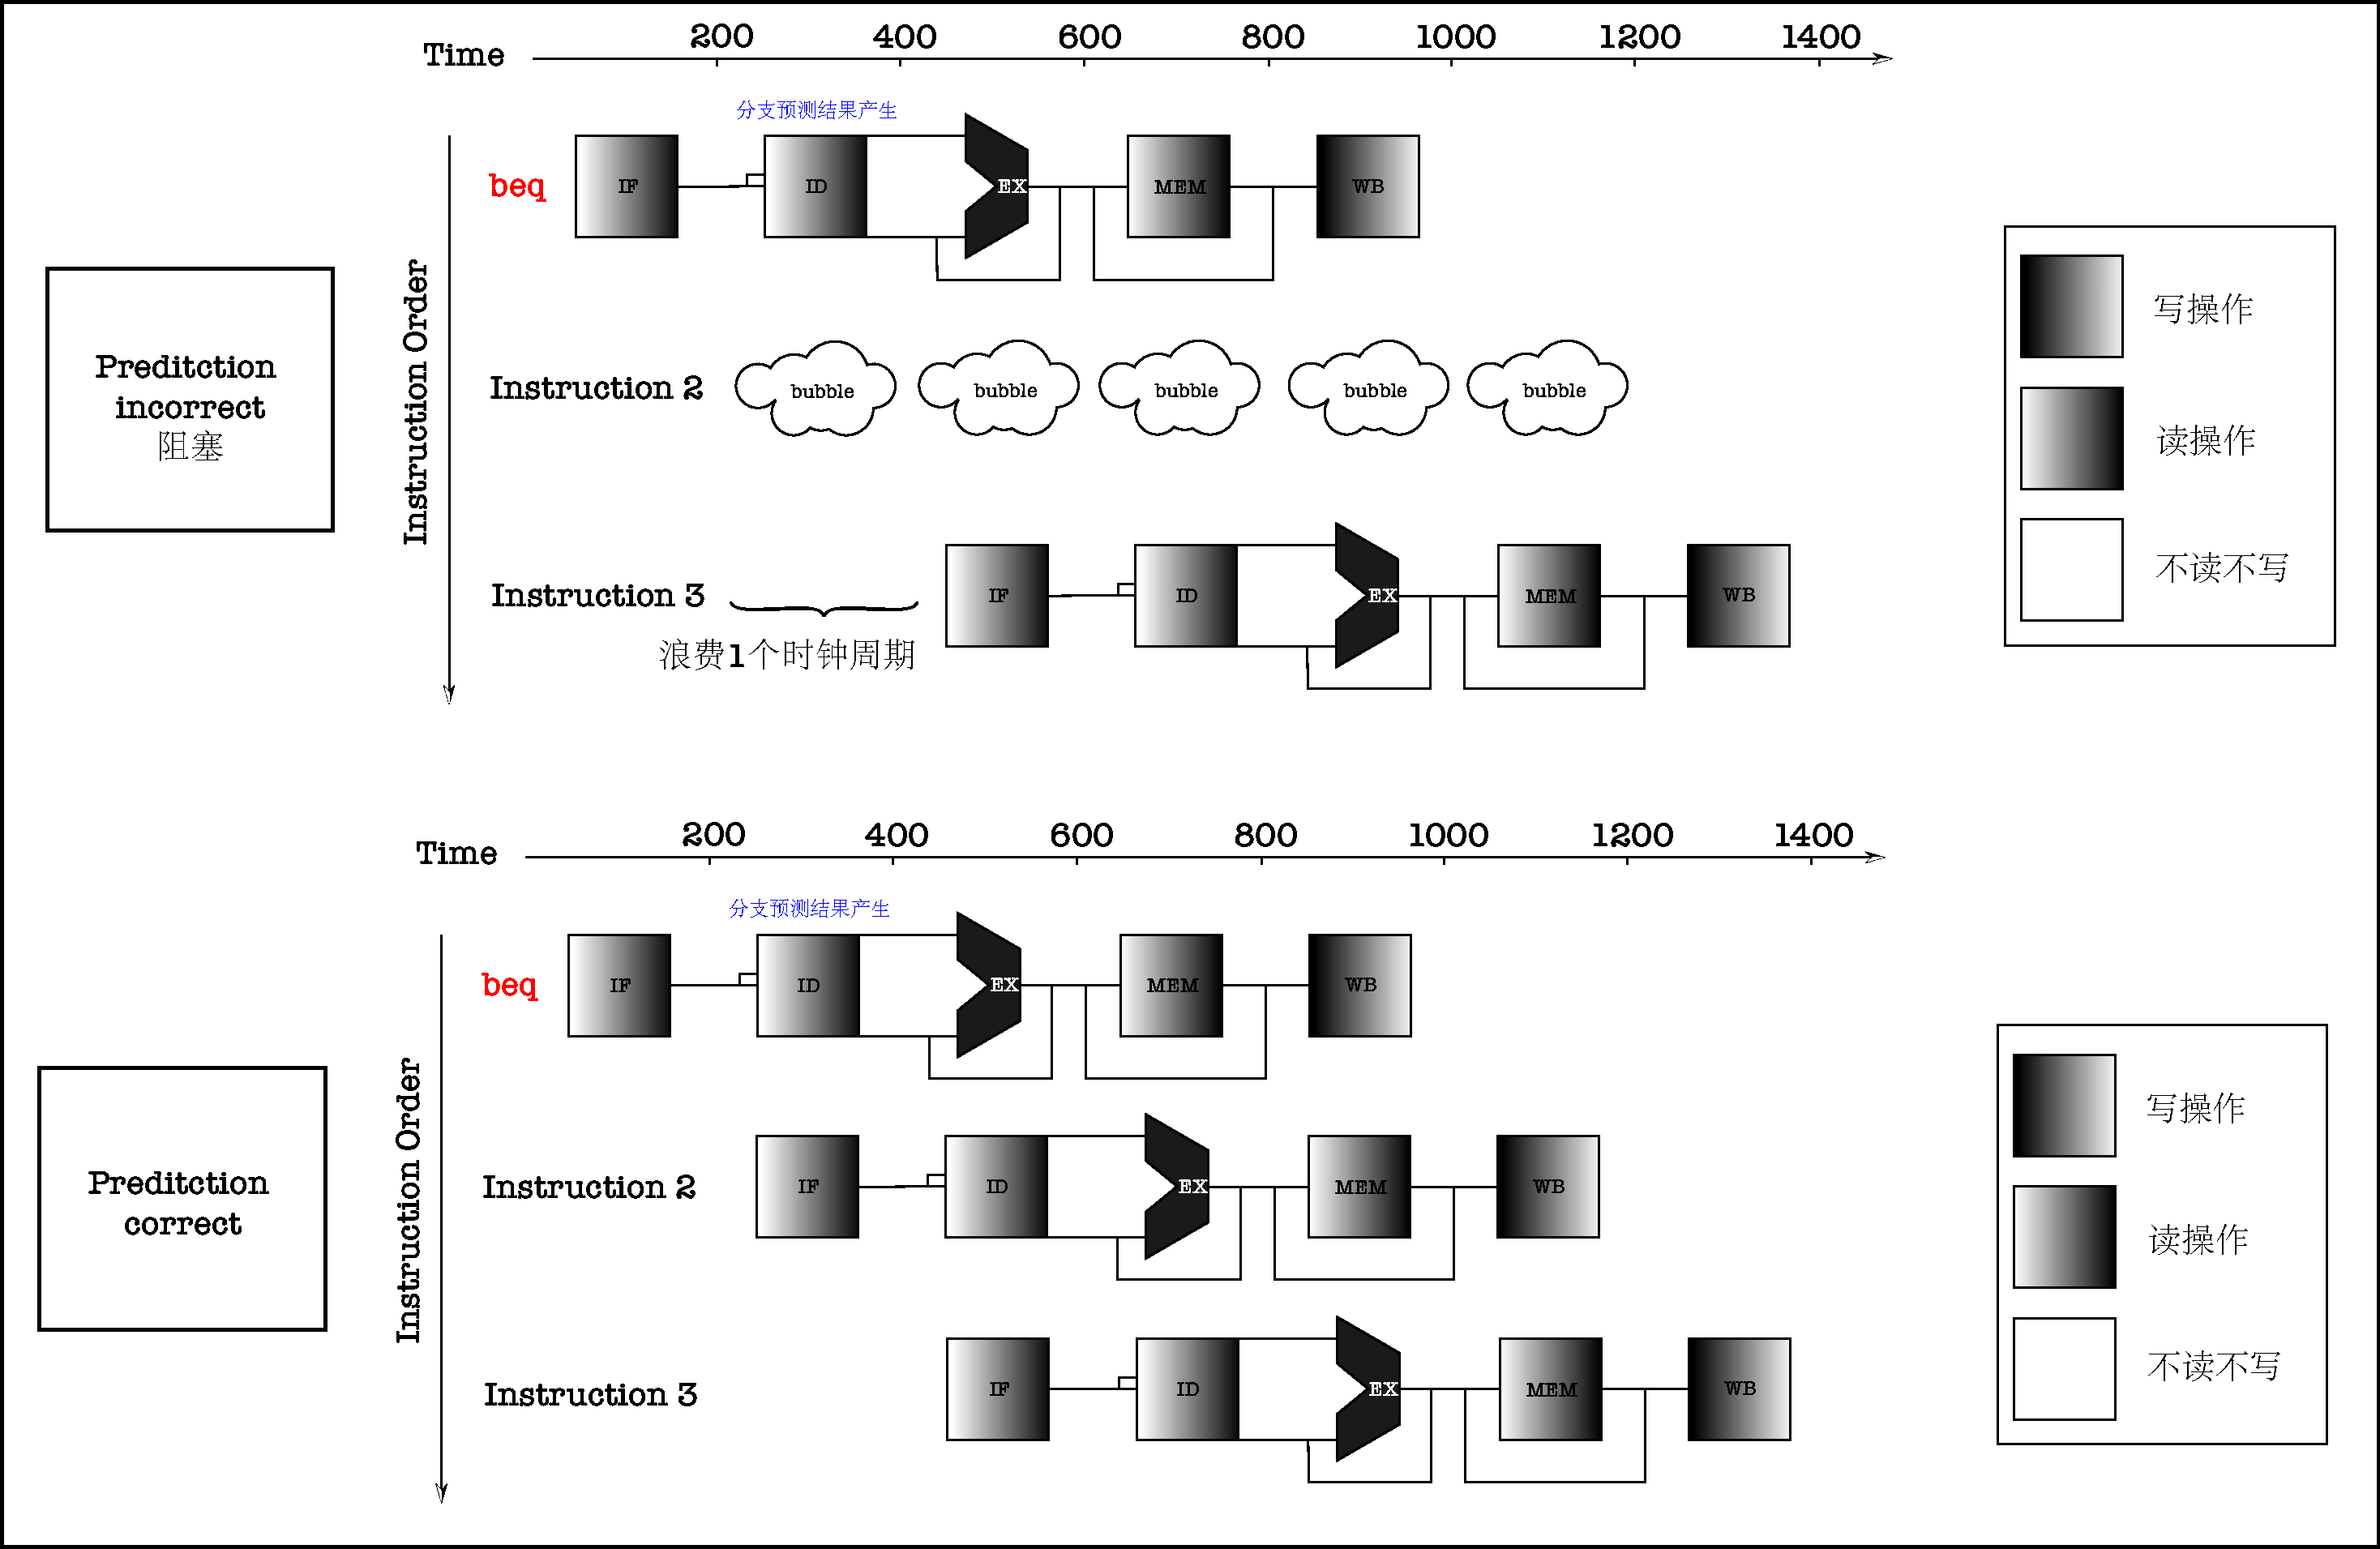
\includegraphics[scale=.35]{img/figure49.pdf}
\end{figure}
除了上述假设分支不发生的预测方法, 还有更加成熟的分支预测方法:
\end{enumerate}
\section{流水线数据通路及其控制}
在前面我们讨论了单时钟周期数据通路, 如下:
\begin{figure}[H]
\centering
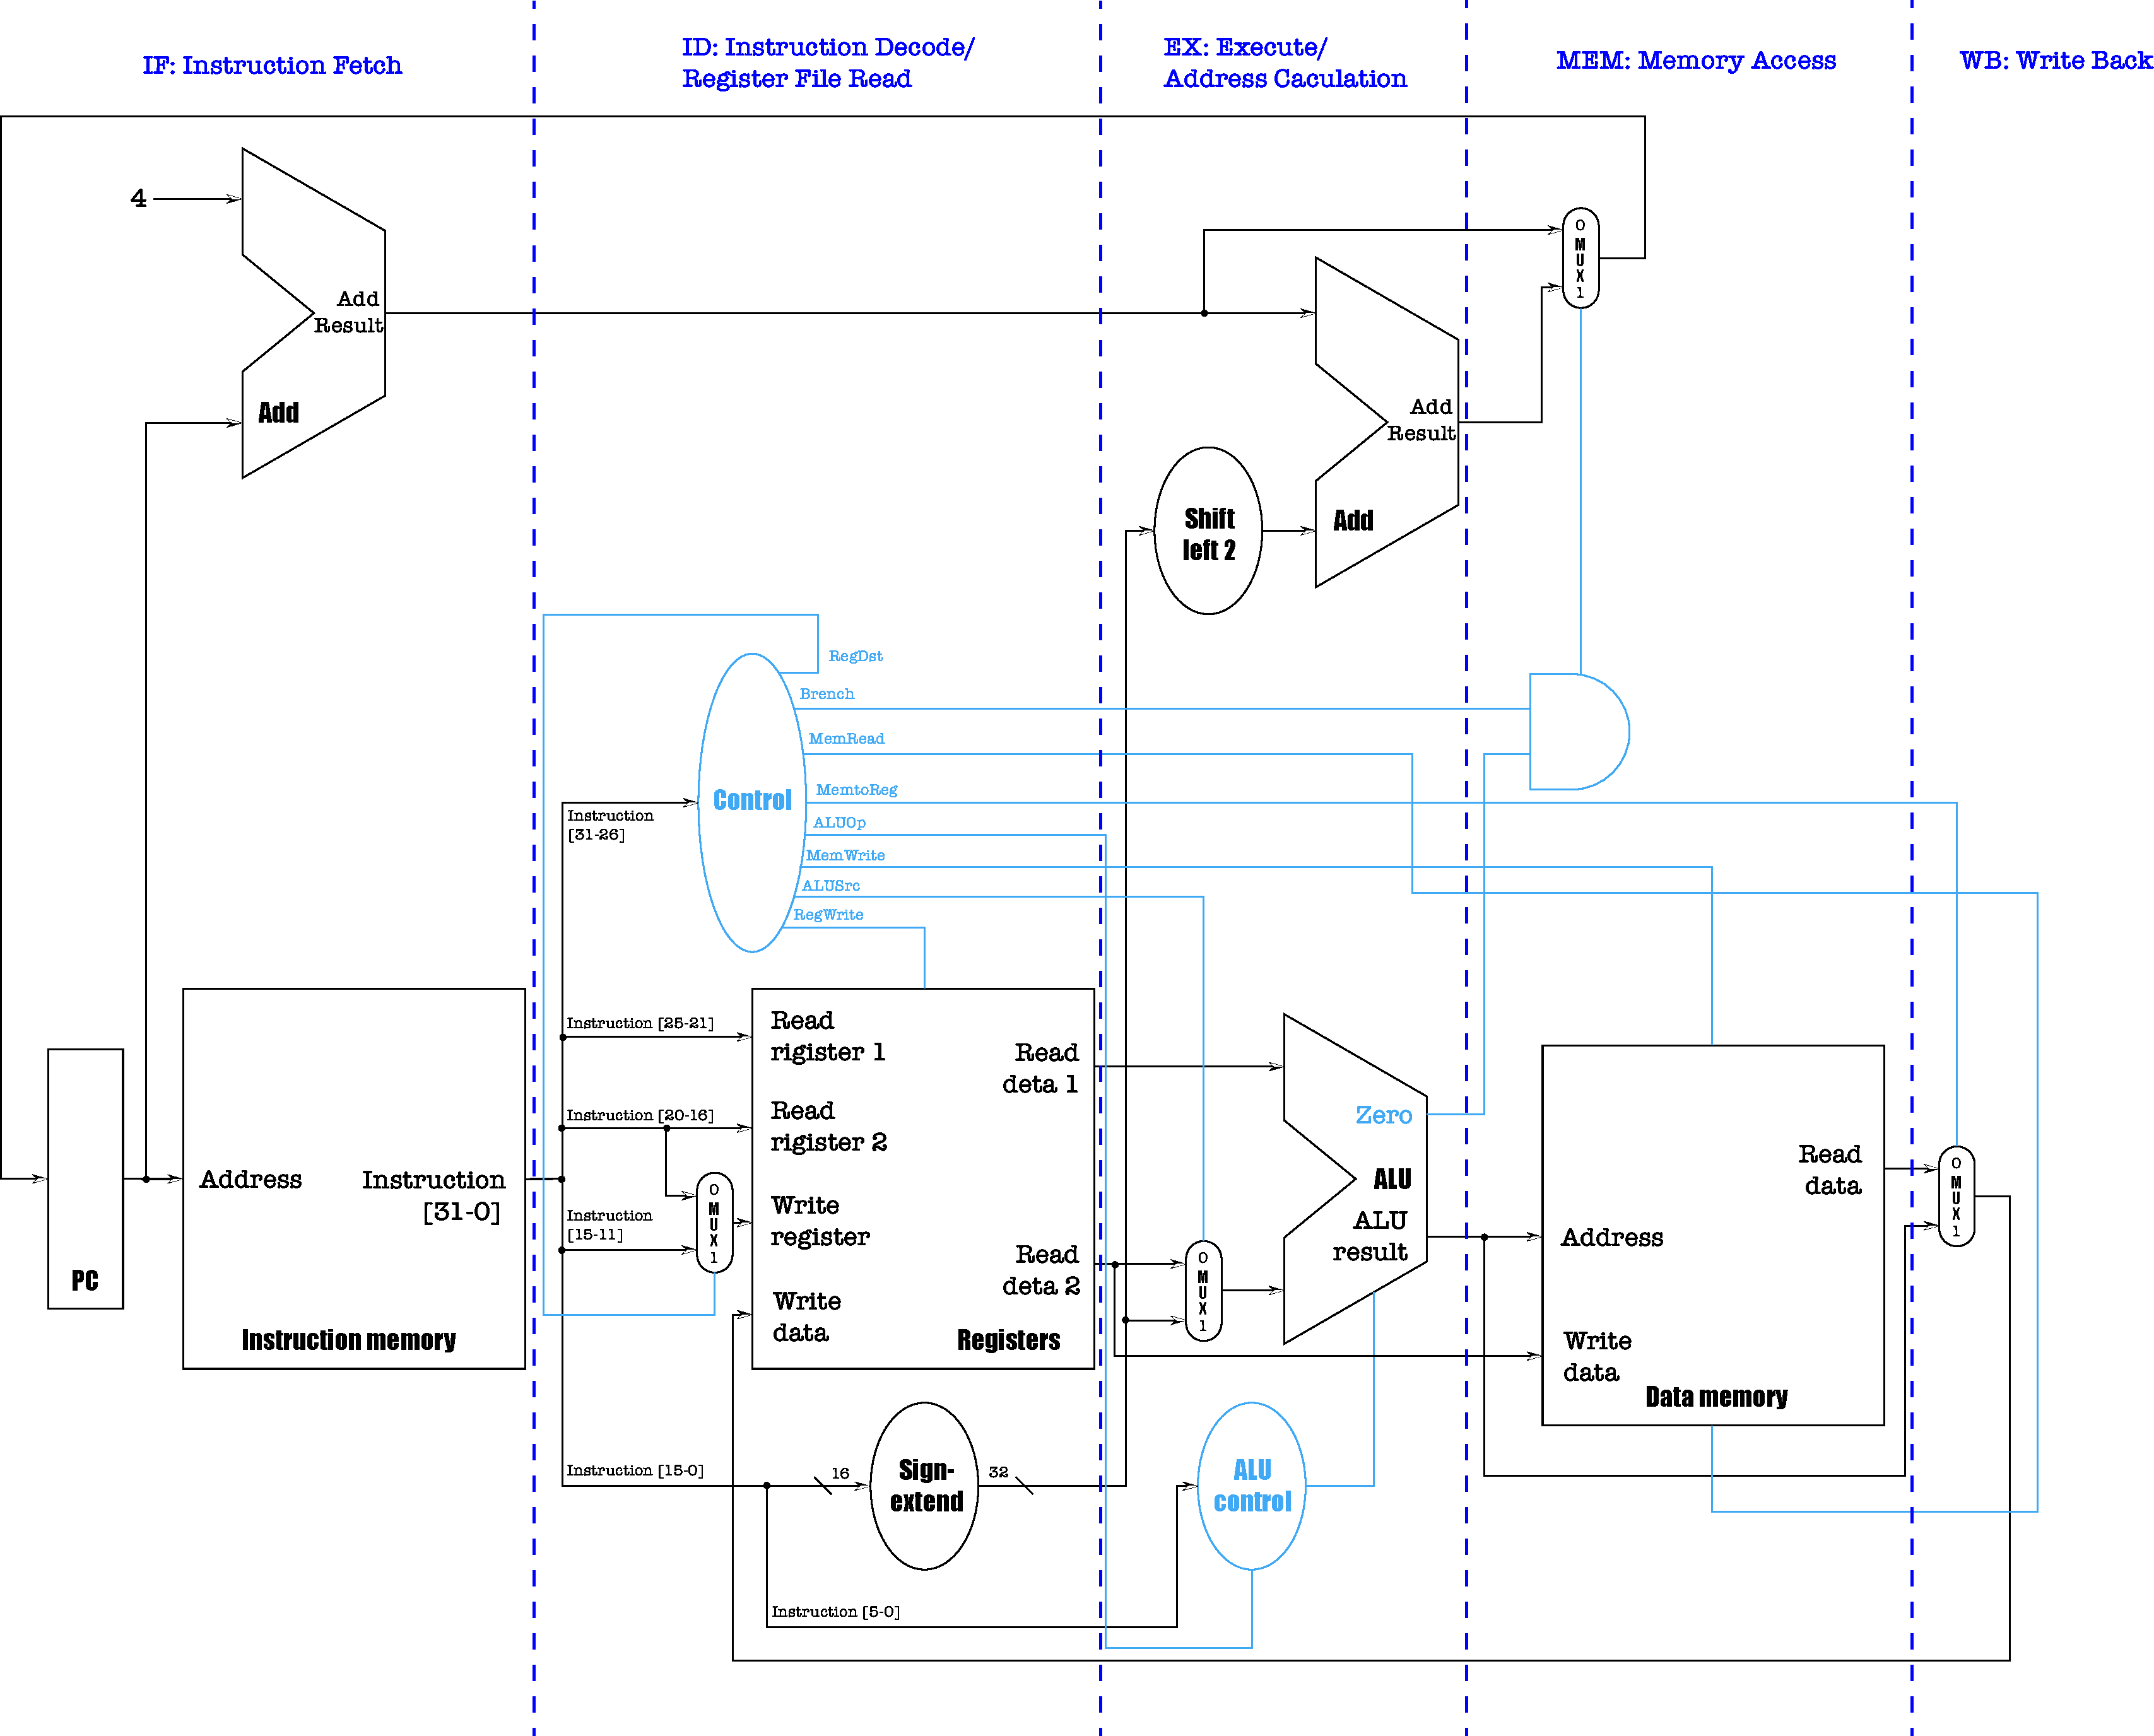
\includegraphics[scale=.2]{img/figure36.pdf}
\end{figure}
我们可以观察到, 图中有两条反向流动的数据:
\begin{itemize}
\item 写回阶段: 把结果写回寄存器堆
\item 选择\verb|PC|的下一个值: 需要在自增的\verb|PC|和\verb|MEM|级的分支地址之间进行选择
\end{itemize}\par
前者将会导致数据冒险, 后者将会导致控制冒险.\par \vspace{1em} 为了实现流水线, 以\verb|IF|为例, \verb|Instruction 1|在执行完\verb|IF|后准备执行\verb|ID|时, \verb|Instruction 2|开始执行\verb|IF|, 从而覆盖掉\verb|Instruction 1|在\verb|IF|阶段的值. 所以相比于单时钟周期的数据通路, 我们需要添加\textbf{流水线寄存器}来保存\verb|Instruction 1|在\verb|IF|阶段的结果. 另外\verb|4|个步骤也是如此. 由此, 我们得到\textbf{数据通路的流水线版本}:
\begin{figure}[H]
\centering
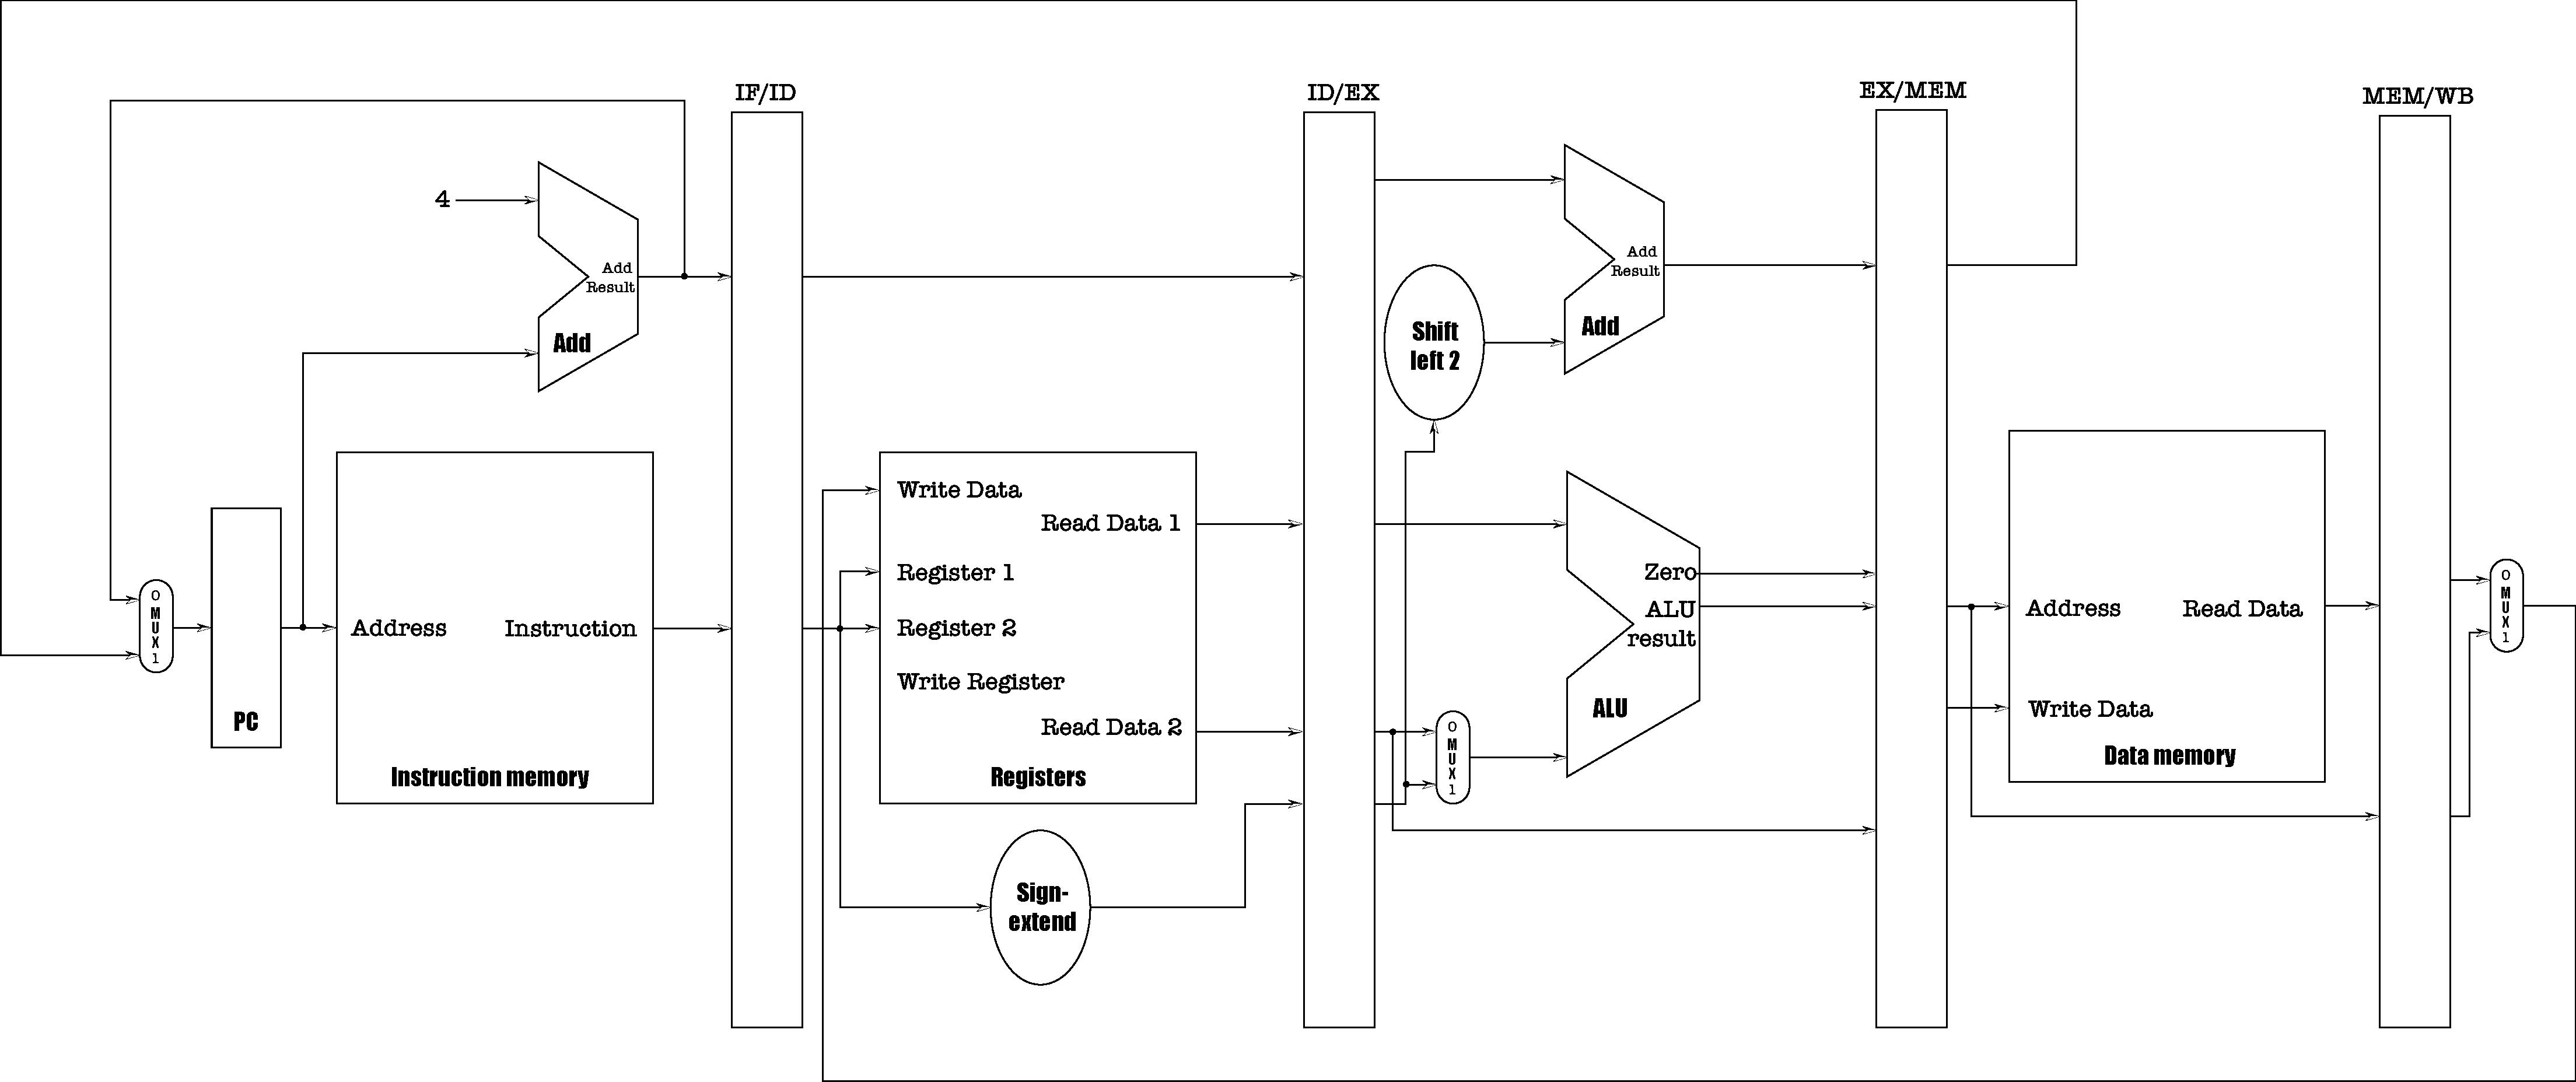
\includegraphics[scale=.2]{img/figure50.pdf}
\end{figure}
\subsection{简单指令的流水线}
\subsubsection{\texttt{lw}指令流水线}
以\verb|lw|指令为例, 分析在流水线中的数据通路:
\begin{enumerate}
\item {\kaishu 取指令} \par 根据\verb|PC|的值, 从指令寄存器中获取到这条指令, 存到\verb|IF/ID|寄存器中. \verb|PC|自增\verb|4|并写回, 等待下一个时钟周期来读取下一条指令, 同时\verb|PC+4|也被存储到\verb|IF/ID|寄存器中, 以备以后使用.
\item {\kaishu 指令译码和寄存器堆的读取} \par 分析指令的各个部分, 读寄存器, 把读到的寄存器值以及扩展后的\verb|32|位偏移值存入\verb|ID/EX|寄存器, 自增后的\verb|PC|也存入\verb|ID/EX|寄存器.
\item {\kaishu 地址计算} \par 把\verb|32|位扩展值以及读寄存器的值用\verb|ALU|相加, 得到目标地址, 将其存入\verb|EX/MEM|寄存器.
\item {\kaishu 存储器访问} \par 用目标地址访问存储器, 把读到的数据存入\verb|MEM/WB|寄存器
\item {\kaishu 写回} \par 把读到的数据写回到寄存器中.
\end{enumerate}\par
分析完\verb|lw|和\verb|sw|中数据流动的特点之后会发现, 这里存在一个\verb|bug|: 写寄存器的这一步发生在整个数据流的最后一步, 要写入寄存器的内容和要写的寄存器号是在最后一步\verb|WB|中给出的. 而上图中, 要写的寄存器号没有随着数据流向后传递, 直到\verb|WB|, 再传回来, 所以我们对电路进行了修正:
\begin{figure}[H]
\centering
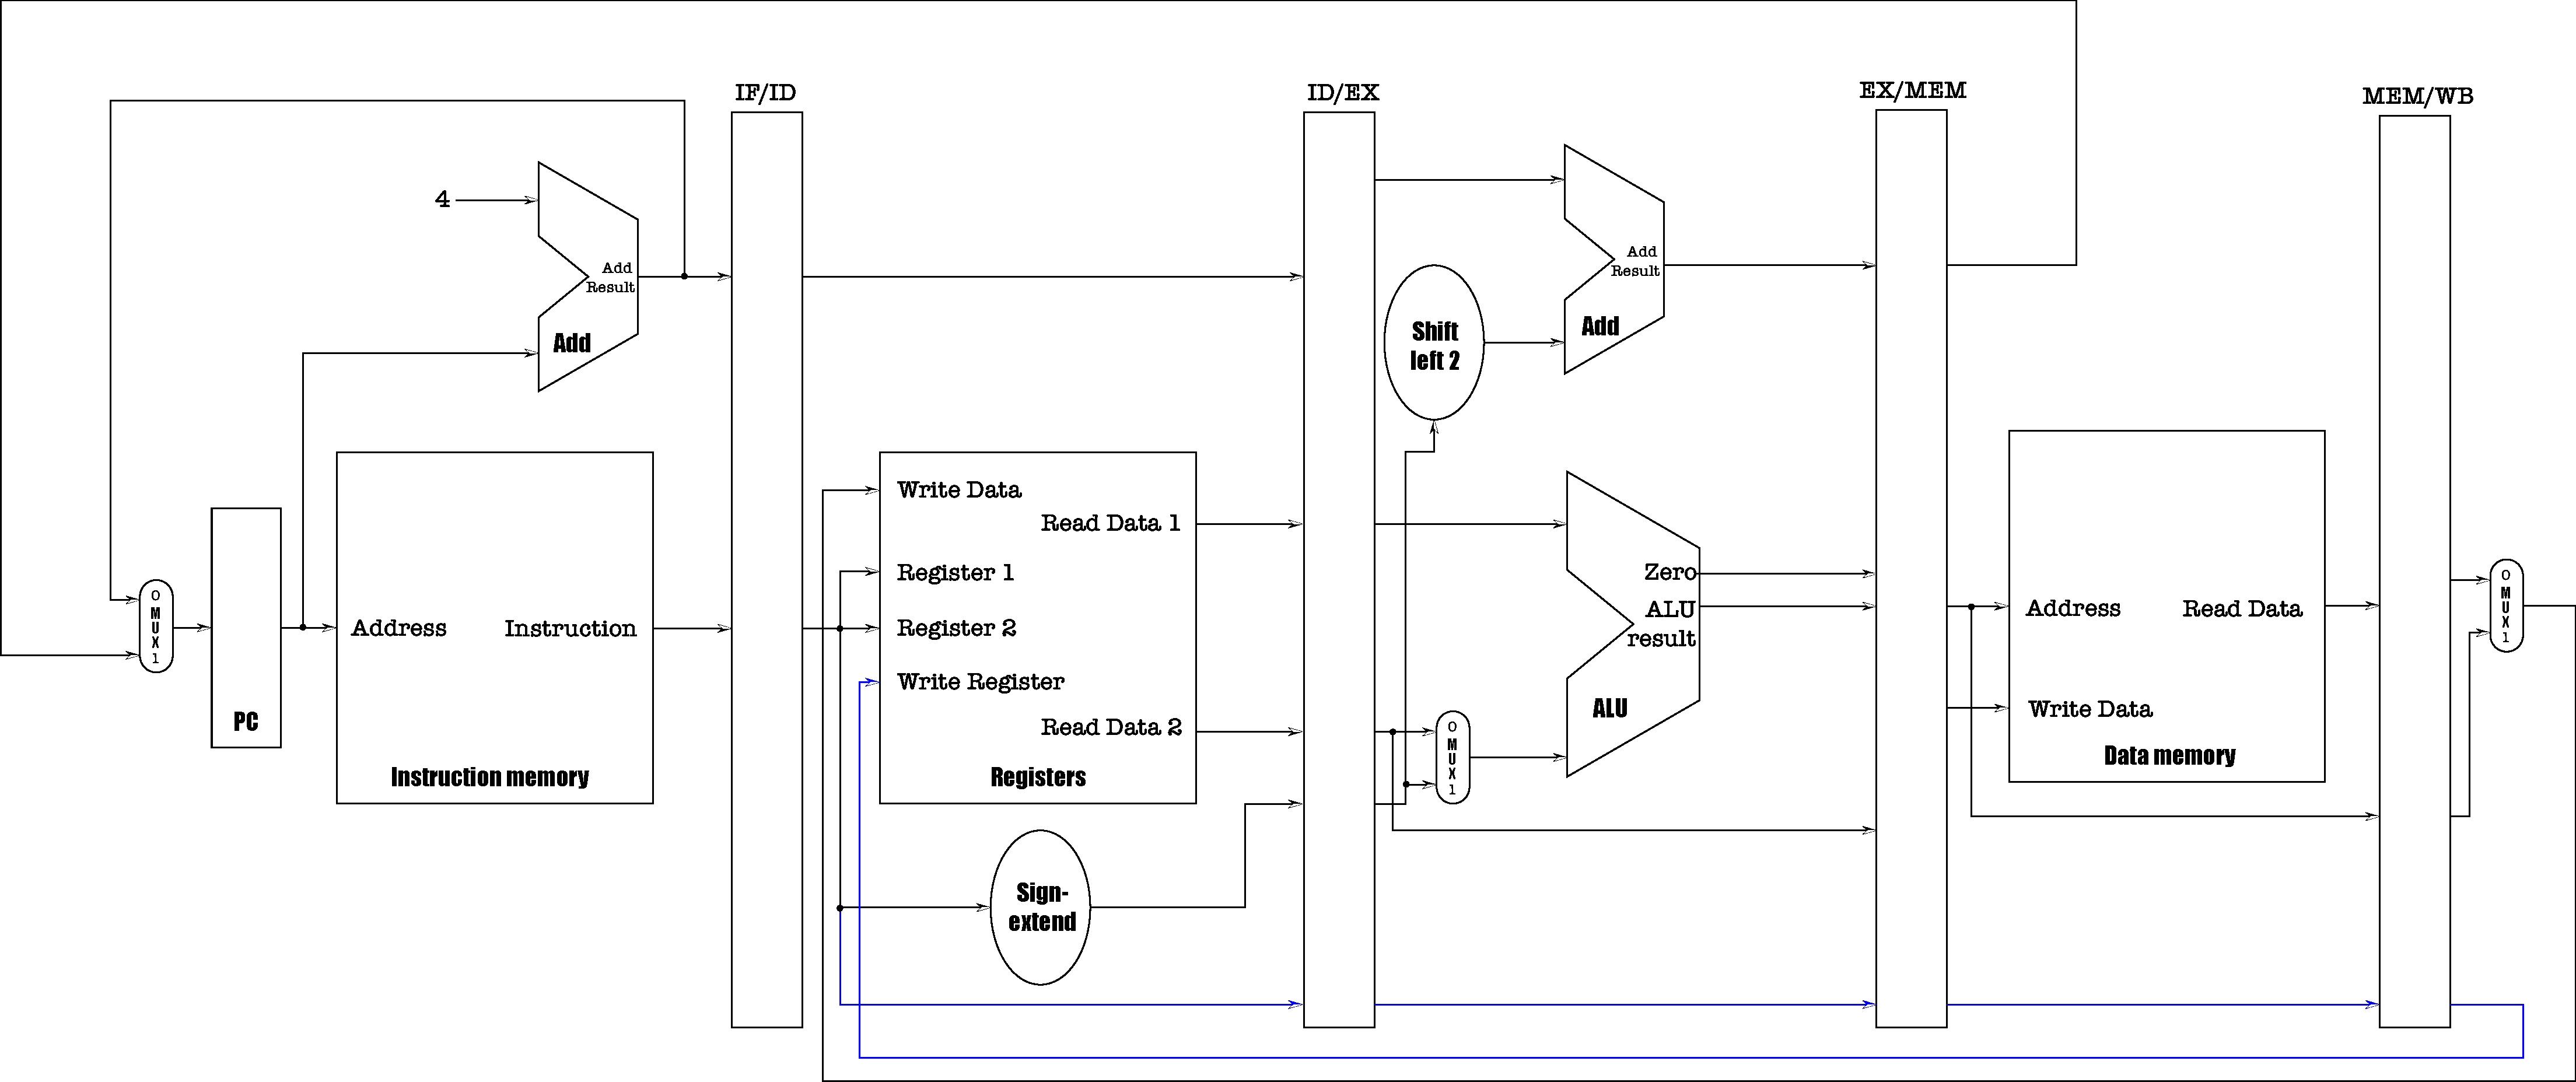
\includegraphics[scale=.2]{img/figure51.pdf}
\end{figure}
\subsubsection{\texttt{sw}指令流水线}
\verb|sw|指令在流水线中的数据通路在\verb|IF|, \verb|ID|步骤与\verb|lw|指令相同. 这里只描述与\verb|lw|指令的不同之处:
\begin{enumerate}
\item {\kaishu 地址计算} \par 它会在\verb|EX/MEM|寄存器中装入要写的数据
\item {\kaishu 存储器访问} \par 数据寄存器是写而不是读
\item {\kaishu 写回} \par 什么也不做
\end{enumerate}
\subsection{流水线控制}
所有的信号均在译码阶段产生并存储在流水线寄存器中. 在设计流水线控制单元的过程中, 研究人员采用了先设计\verb|ALU Control|, 再设计其他控制信号的方式:
\subsubsection{\texttt{ALU Control}设计}
\verb|ALUOp|取决于指令的\verb|opcode|和某些\verb|funct|.
\begin{figure}[H]
\centering
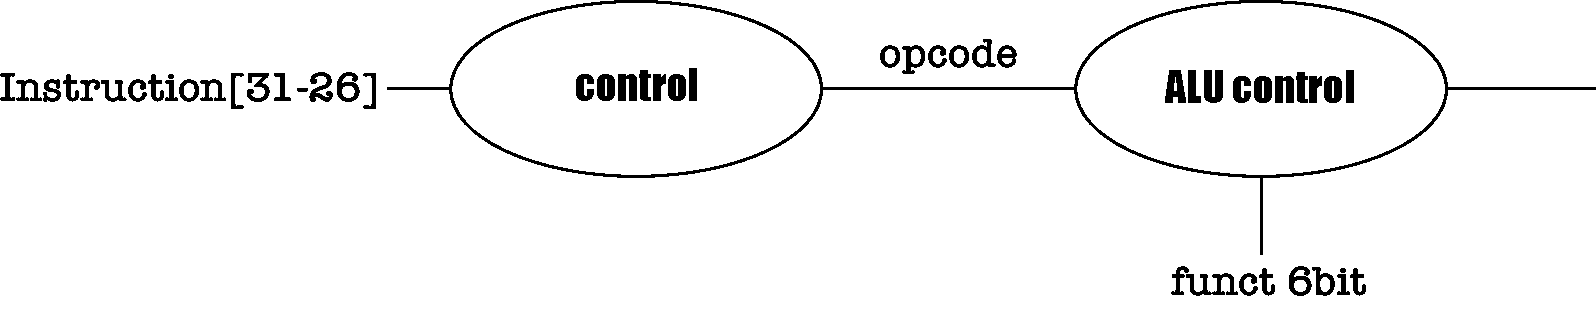
\includegraphics[scale=.5]{img/figure52.pdf}
\end{figure}
上图采用的是多级译码的方式, 降低了主控单元复杂度.
\subsubsection{其他控制信号单元设计}
其他控制信号包括\textcolor{myred}{多选器控制信号}, \textcolor{myblue}{存储器读写控制信号}, \textcolor{mygreen}{间接信号}(如\verb|Branch|信号要和\verb|ALU|结果比较).
\begin{table}[H]
\centering
\begin{tabularx}{\textwidth}{|X|X|X|}
\hline
\makecell*[c]{\textbf{控制信号名称}} & \makecell*[c]{\textbf{无效含义}} & \makecell*[c]{\textbf{有效含义}} \\ \hline
\makecell*[c]{\textcolor{myred}{\texttt{RegDst}}} & \makecell*[l]{写寄存器的目标寄存器号来自\\\texttt{rt}字段(\texttt{Ins[20-16]})} & \makecell*[l]{写寄存器的目标存储器号来自\\\texttt{rd}字段(\texttt{Ins[15-11]})} \\ \hline
\makecell*[c]{\textcolor{myred}{\texttt{ALUSrc}}} & \makecell*[l]{第二个\texttt{ALU}操作数来自\\寄存器堆的第二个输出} & \makecell*[l]{第二个\texttt{ALU}操作数来自指令\\低\texttt{16}位的符号位扩展后的\\\texttt{32}位数} \\ \hline
\makecell*[c]{\textcolor{myred}{\texttt{MemtoReg}}} & \makecell*[l]{写入寄存器的数来自\texttt{ALU}} & \makecell*[l]{写入寄存器的数来自数据\\寄存器} \\ \hline
\makecell*[c]{\textcolor{myblue}{RegWrite}} & \makecell*[l]{无} & \makecell*[l]{寄存器堆写有效} \\ \hline
\makecell*[c]{\textcolor{myblue}{MemRead}} & \makecell*[l]{无} & \makecell*[l]{数据存储器读有效} \\ \hline
\makecell*[c]{\textcolor{myblue}{MemWrite}} & \makecell*[l]{无} & \makecell*[l]{数据存储器写有效} \\ \hline
\makecell*[c]{\textcolor{mygreen}{\texttt{PCSrc}}} & \makecell*[l]{\texttt{PC}由\texttt{PC+4}取代} & \makecell*[l]{\texttt{PC}由分支目标取代} \\
\hline
\end{tabularx}
\end{table}







